\documentclass[a4paper]{article}

%% Language and font encodings
\usepackage[utf8x]{inputenc}
%\usepackage[T1,T2A]{fontenc}
\usepackage[english, russian]{babel}

%% Sets page size and margins
%\usepackage[a4paper,top=3cm,bottom=2cm,left=3cm,right=3cm,marginparwidth=1.75cm]{geometry}

\usepackage {amssymb}
\usepackage{amsmath}
\usepackage{floatrow, graphicx, calc}
\usepackage{subcaption}
%\usepackage[dvips]{graphicx}
%\usepackage[colorinlistoftodos]{todonotes}
%\usepackage[colorlinks=true, allcolors=blue]{hyperref}

%\bibliographystyle{ugost2003}
%\bibliographystyle{abbrv}

\sloppy

\topmargin =-10mm \textwidth =170mm \textheight =230mm
\oddsidemargin =-3mm


\title{Клиновидный биллиард в постоянном поле}
\author{Ю.Н. Масловcкий, В.В. Яновский}

\begin{document}
\maketitle

\begin{abstract}
Рассмотрено движение заряженной частицы в постоянном поле в клине при упругом отражении ее от границ. Введено естественное фазовое пространство и выяснены его свойства. Аналитически получено динамическое отображение, определяющее движение точки в фазовом пространстве. Установлены типичные свойства траекторий и общие характерные особенности фазовых портретов.
\end{abstract}

\section{Введение}

В работе рассматривается движение массивной материальной точки в плоском клиновидном биллиарде под действием постоянного гравитационного поля (либо заряженной массивной частицы под действием постоянного электрического поля). Основное внимание сосредоточено на случае общего положения -- несимметричного клина. Ось симметрии такого клина (биссектриса) расположена произвольным образом относительно направления поля (см. Рис. \ref{fig:in1}), а не параллельно, как в симметричном случае.  Раннее симметричный случай был рассмотрен в работах \cite{Lehtihet1986,Sepulchre2003}.  К биллиарду в клине сводится одномерная задача о трех гравитирующих  плоскостях, которая упоминается в \cite{Lehtihet1986}. В статье \cite{Sepulchre2003} рассматривается стабилизация периодических орбит в клиновидном биллиарде.  Однако обе статьи ограничиваются симметричным случаем.

В статье \cite{Yanovskii2013}  рассматривалось поведение массивной частицы в треугольнике в гравитационном/электрическом поле. Был применен новый геометрический подход, который мы разовьем в данной статье.


\section{ Клиновидный биллиард }

Рассмотрим равноускоренное движение частицы в $R^{2} $. При этом частица упруго сталкивается с границей, образованной двумя пересекающимися прямыми.
%\begin{figure}[ht]
%  \centering
% 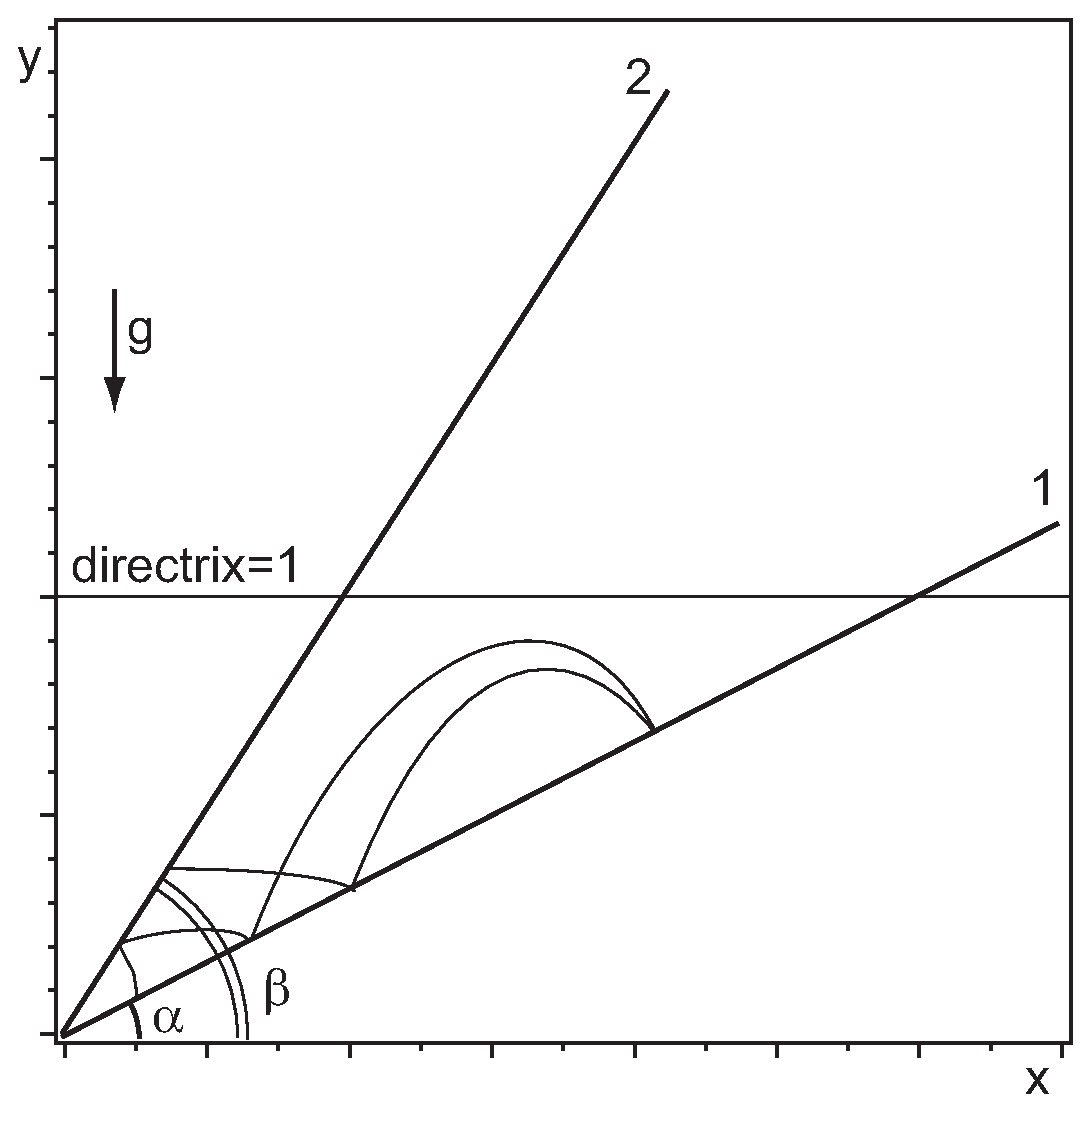
\includegraphics[width=.4]{in3n}\\
%  \caption{Показано расположение клина и пример части траектории в нем. Также показано расположение директрисы парабол. Направление поля вертикально вниз как и ранее.}\label{image4}
%\end{figure}

%\begin{figure}
%  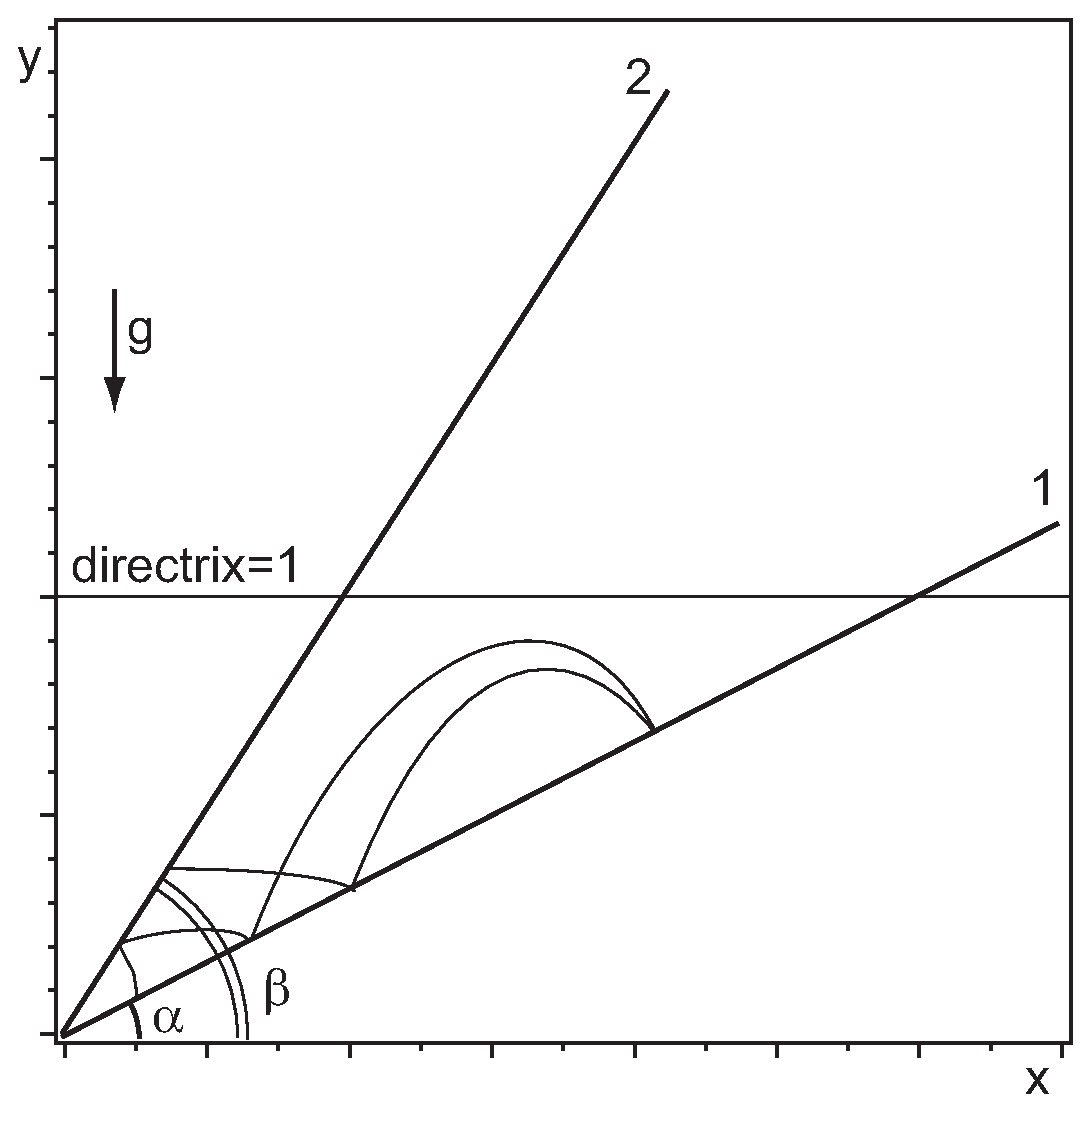
\includegraphics[width=\linewidth]{in3n}
%  \caption{Показано расположение клина и пример части траектории в нем. Также показано расположение директрисы парабол. Направление поля вертикально вниз как и ранее.}
%  \label{image4}
%\end{figure}

\begin{figure}[h]
\center{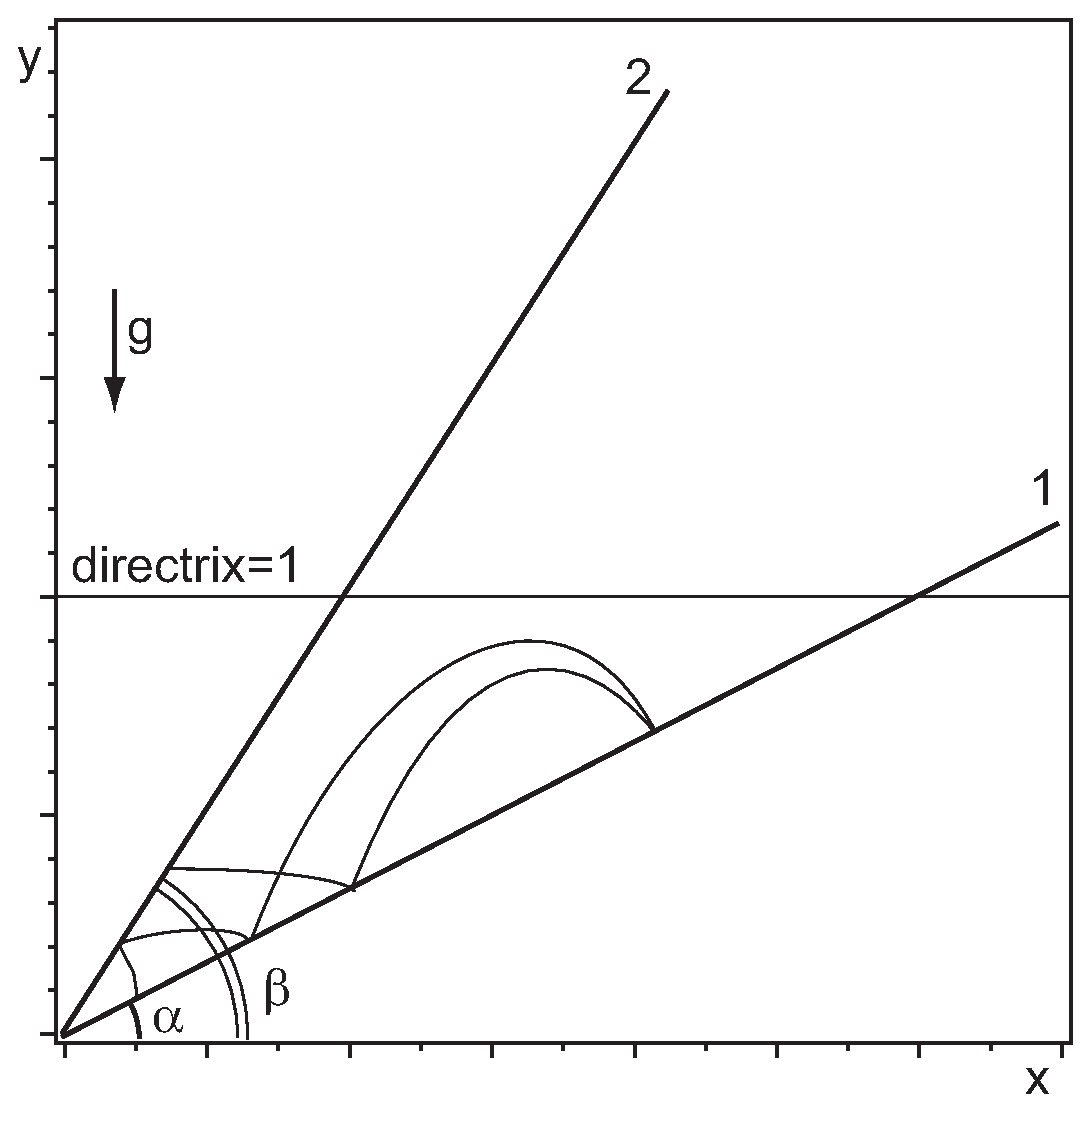
\includegraphics[width=0.3\linewidth]{in3n}}
\caption{Показано расположение клина и пример части траектории в нем. Также показано расположение директрисы парабол. Направление поля вертикально вниз как и ранее.}
\label{image4}
\end{figure}
На Рис.\ref{image4} изображен один из вариантов такого клина, соответствующего условию для стенок $0<\alpha <\beta <{\raise0.7ex\hbox{$ \pi  $}\!\mathord{\left/ {\vphantom {\pi  2}} \right. \kern-\nulldelimiterspace}\!\lower0.7ex\hbox{$ 2 $}} $. Углы отсчитываются стандартно от оси $y$ против часовой стрелки. Пронумеруем стенки с углами наклона $\alpha $ и $\beta $ как 1 и 2, соответственно.


% Рис.1
Как известно, траектория свободной равноускоренной частицы в общем случае представляет собой параболу. Поэтому траектория в клине или в любой другой ограниченной области, представляет собой последовательность сегментов парабол, которые \textit{полностью} лежат внутри этой области. Каждый из сегментов имеет точку пересечения, как с предыдущим, так и с последующим сегментами, и эти точки пересечения для всех сегментов лежат на границе области. В рассматриваемом случае -- на стенках клина. Поскольку парабола задается фокусом и директрисой, то представляется естественным, при наличии общей постоянной директрисы, рассмотреть эволюцию именно фокусов парабол, соответствующих сегментам траекторий. Назовем такое отображение фокусным.


Движение такой частицы будет ограничено двумя наклонными стенками (клином), а сверху общей директрисой всех возможных траекторий частицы с заданной полной энергией (см. Рис.\ref{image4}). Без ограничения общности можно положить директрису равной единице.


 Если оставим одну бесконечную стенку, то в получим два варианта отражения частицы при падении. В одном случае она  падает на нее снова, а во втором уходит на бесконечность (кроме частного случая вертикальной стенки, где всегда не больше одного отражения).
%  Это связано с особенностью пересечения параболы с прямой, которая делит параболу на три сегмента. Средний сегмент начинается и заканчивается на той же прямой и при отражении тип сегмента поменяться не может. 
 Назовем первый вариант падения - нижней стенкой, а второй - верхней. Если мы определим вектор нормали к стенке как совпадающий с направлением нормальной составляющей скорости отраженной частицы, то для любого клиновидного биллиарда это направление для каждой из стенок будет фиксированным. При этом легко показать, что для нижней стенки вертикальная составляющая нормали всегда $n_y>0$ и соответственно для верхней $n_y<0$. На  Рис.\ref{image4} изображен вариант где 1 стенка является нижней, а 2 - верхней. При этом ясно, что в случае падения на 2 стенку, следующее падение будет обязательно на 1-ю стенку, тогда как падение на 1-ю не гарантирует падение на 2-ю.
% Особенностью данного расположения стенок является то, что частица \textit{всегда} после столкновения со 2-й стенкой далее падает на 1-ю. Тогда как после падения на 1-ю стенку частица может, как столкнуться со 2-й, так и снова столкнутся с 1-й. Т.е. вообще говоря существует два разных варианта падения на одну и ту же стенку.


\section{Фокусное отображение наклонной стенки}

Рассмотрим фокусное отображение при падении частицы на наклонную стенку на заданном ограниченном участке $A_{1} A_{2} $ (см. Рис.~\ref{image5}). Уравнение стенки задается уравнением $y=x\; tg{\kern 1pt} \alpha +b$, а директриса $y=1$. Фокус начального сегмента траектории обозначим как $F$. Введем естественный параметр $l$ для любой точки ограничивающего отрезка, как расстояние от точки $A_{1} \left(x_{1} ,y_{1} \right)$ до точки отрезка $K\left(x,y\right)$. Тогда легко найти в естественной параметризации $x=x_{1} +l\cos \, \alpha ,\quad y=x_{1} \, tg\, \alpha +l\sin \, \alpha +b$. Таким образом, $l\in \left[0,\, l_{2} \right]$, где $l_{2} $ соответствует точке $A_{2} $. Исходя из условия, что парабола $F$ должна обязательно пересекать отрезок $A_{1} A_{2} $, мы можем построить область определения фокусного отображения на отрезке. Для этого найдем точки пересечения параболы с направляющей прямой отрезка. Это легко сделать из геометрического определения параболы как геометрического места точек равноудаленного от фокуса и директрисы, а также условия пересечения параболы с наклонной стенкой

\begin{equation} \label{GrindEQ__1_} \left(X-x\right)^{2} +\left(Y-y\right)^{2} =\left(1-y\right)^{2}  , y=x\; tg{\kern 1pt} \alpha +b \end{equation}

Решая совместно эти уравнения, и переходя далее к естественной параметризации $l$, получим точки пересечения.

\begin{equation} \label{GrindEQ__2_}  l_{\pm } =\frac{1}{\cos ^{2} \alpha } \left(\left(X-x_{1} \right)\cos \, \alpha -\left(1-Y\right)\sin \, \alpha \pm \sqrt{\left(1-Y\right)d\left(X,Y,\alpha ,b\right)} \right)\end{equation}

\[d\left(X,Y,\alpha ,b\right)={\rm 1\; -\; b\; -\; (b\; -\; Y)\; cos}\, {\rm 2}\alpha {\rm \; -\; X\; sin}\, {\rm 2}\alpha \]

На Рис. 2 значения $l_{\pm } $ соответствуют точкам $K_{+} $и $K_{-} $.

%\begin{figure}[ht]
%  \centering
% 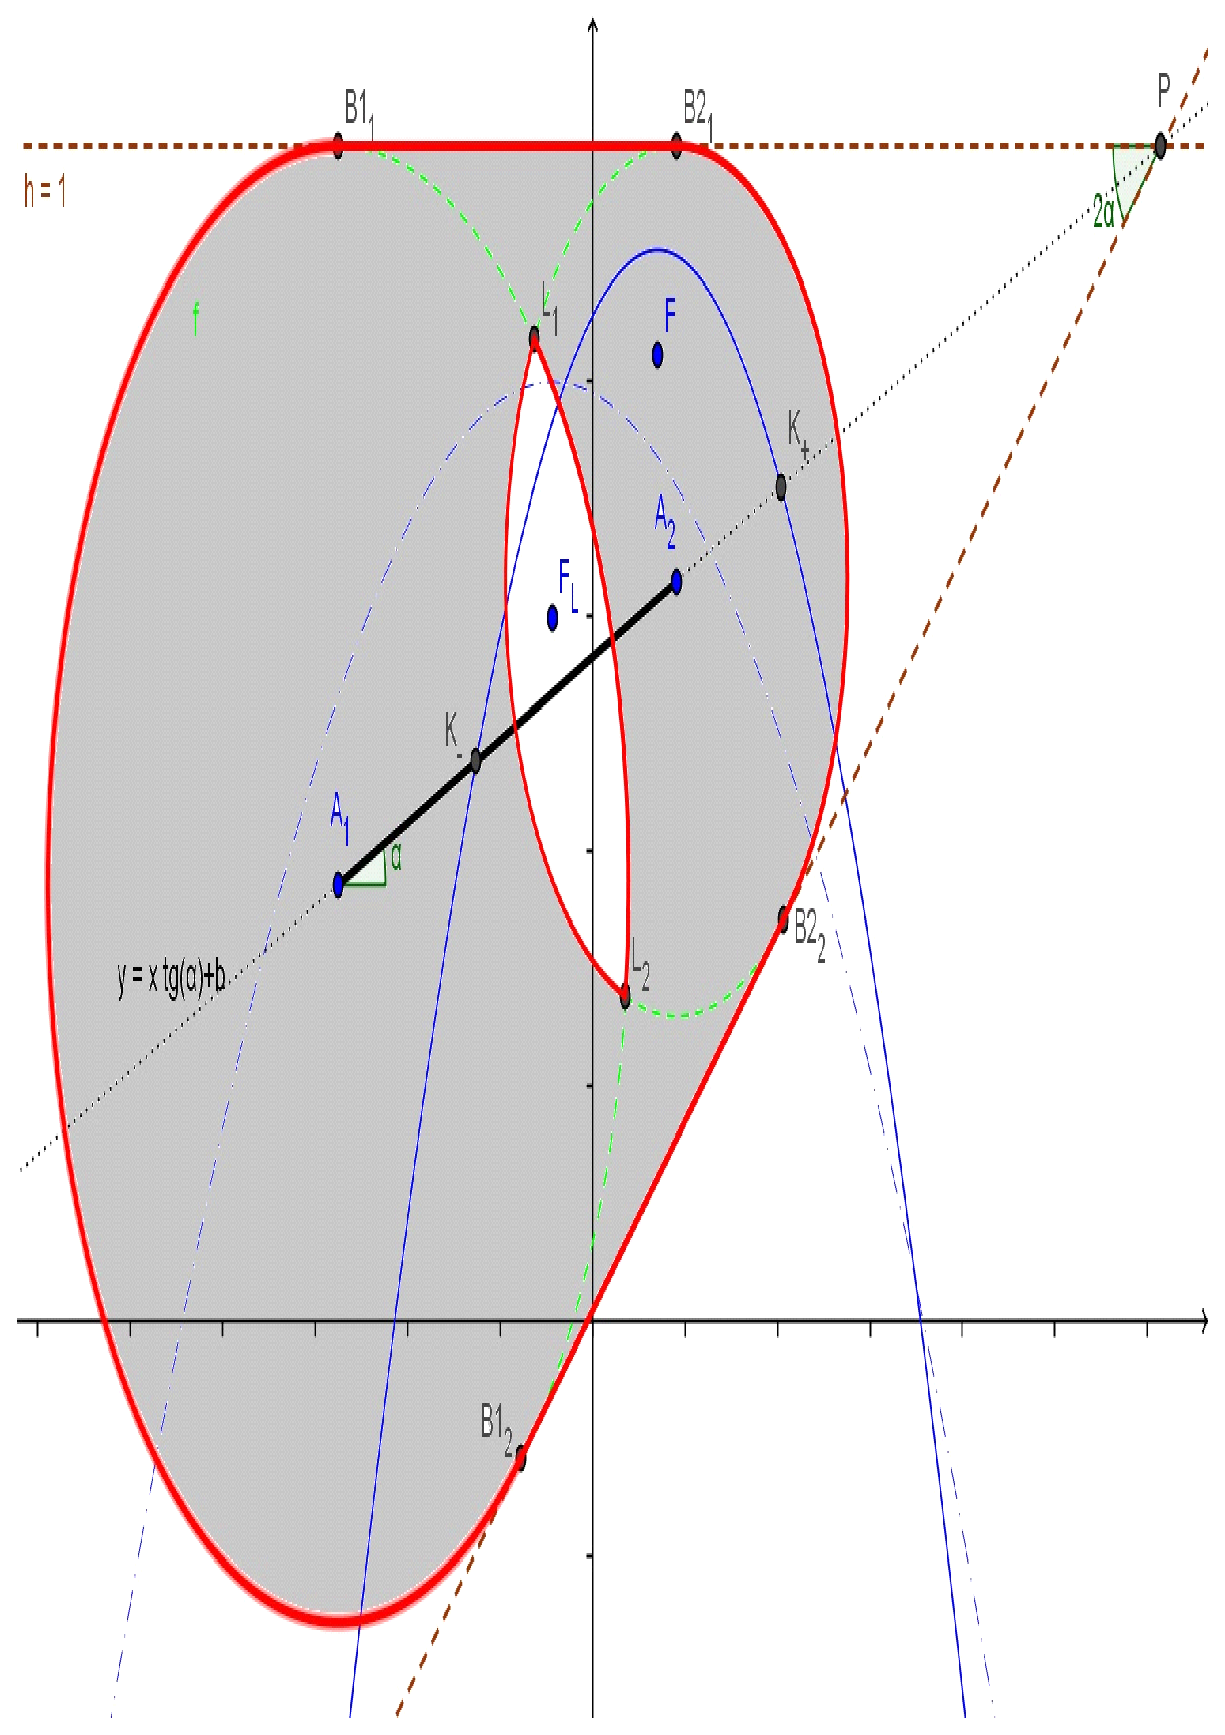
\includegraphics[width=143.6mm, height=80.7mm, viewport=3mm 4mm 205mm 292mm]{image5}\\
%  \caption{}\label{image5}
%\end{figure}

\begin{figure}[h]
\center{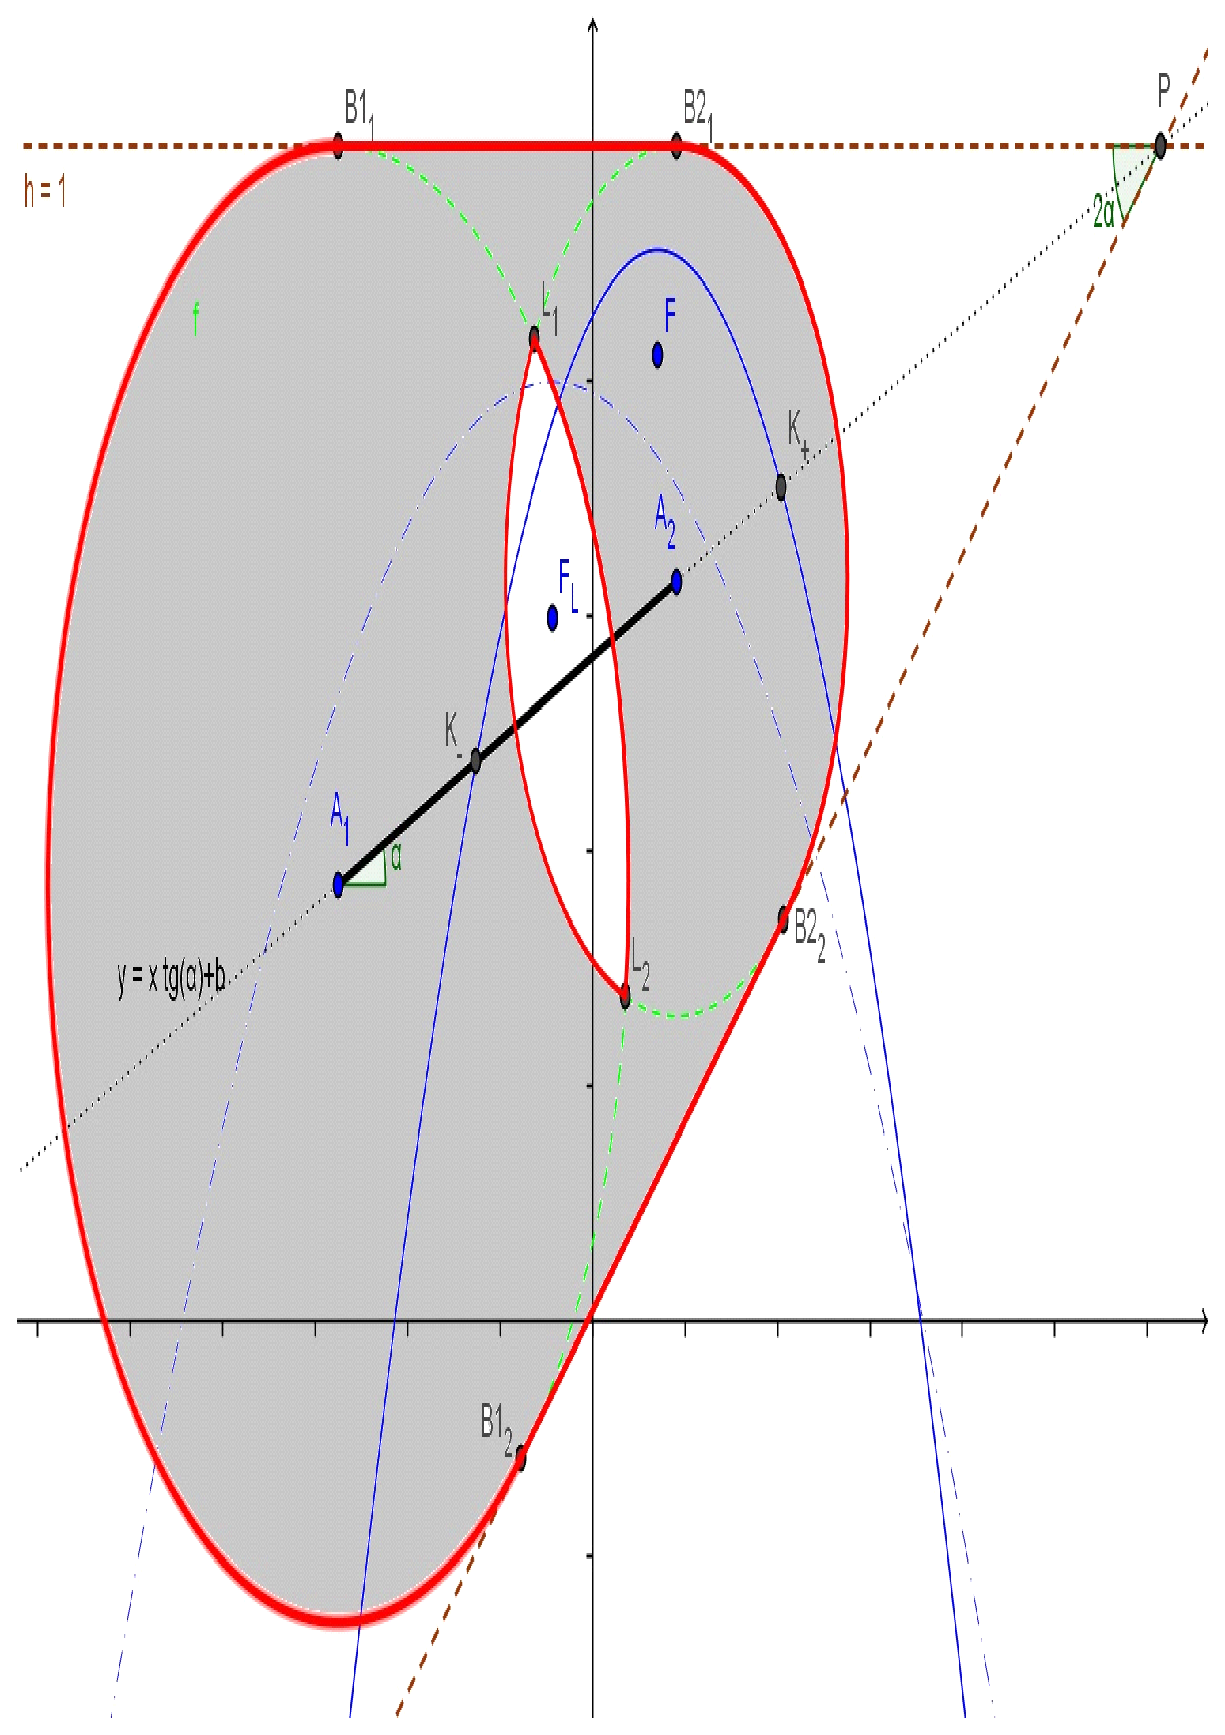
\includegraphics[width=.7\linewidth]{image5}}
\caption{Изображена область определения с лакуной для фокусного отображения на стенке в виде отрезка.}
\label{image5}
\end{figure}

Из \eqref{GrindEQ__2_} ясно, что подкоренное выражение должно быть не меньше нуля. Учитывая далее, что $Y\le 1$, т.е. фокус должен лежать ниже директрисы, получаем первые два условия области определения

\begin{equation} \label{GrindEQ__3_} Y\le 1,  1-b+\left(Y-b\right)\cos \, 2\alpha -X\sin \, 2\alpha \ge 0 \end{equation}

Чтобы понять чему соответствует вторая область, проведем дополнительные построения (см. Рис.\ref{image5}). Проведем из точек $A_{1} $ и $A_{2}$ окружности касательные  к директрисе. Из точки пересечения $P$ директрисы с наклонной стенкой, проведем вторую касательную (первая -- это сама директриса по построению) к построенным окружностям. Область, лежащая выше этой прямой, и будет искомой. Отметим простой геометрический смысл $d\left(X,Y,\alpha ,b\right)$ из \eqref{GrindEQ__2_} есть просто расстояние от фокуса до этой касательной, $1-Y$ -- расстояние до директрисы.

Также можно показать, что неравенства $l_{+} \ge 0$ и  $l_{-} \le l_{2} $, соответствуют дополнительной области определения фокусов возможных парабол. Кроме того, в полученной области определения может присутствовать лакуна (см. Рис.\ref{image5}) когда одновременно выполняются условия  $l_{-} \le 0$ и $l_{+} \ge l_{2} $, что соответствует пересечению окружностей  $A_{1} $ и $A_{2} $, когда $l_{2} $ меньше суммы радиусов упомянутых окружностей. Т.е. $l_{2} \le \left(1-y_{1} \right)+\left(1-y_{2} \right)=2\left(1-b\right)-2x_{1} \, tg\, \alpha -l_{2} \sin \, \alpha $. Отсюда, приравнивая левую и правую части неравенства находим длину отрезка, которая соответствует появлению лакуны (окружности $A_{1}$ и $A_{2}$ касаются друг друга на стенке).

\begin{equation} \label{GrindEQ__4_} l_{2} =2\frac{1-b-x_{1} tg\, \alpha }{1+\sin \, \alpha }  \end{equation}

%Особый интерес представляет область определения для двух и более отрезков. Обозначим области соответствующие отрезкам $A_{1} A_{2} $ и $B_{1} B_{2} $ как $A$ и$B$, соответственно (см. Рис.\ref{image6_7}а). Ясно, что область определения в этом случае представляет собой объединение областей каждого из них и, как видно на Рис. 2а, эти области не пересекаются. Далее, сближая отрезки  параллельным переносом вдоль оси $x$, области начинают перекрываться (Рис.~\ref{image6_7}б).
%
%\begin{figure}[ht]
%  \centering
%  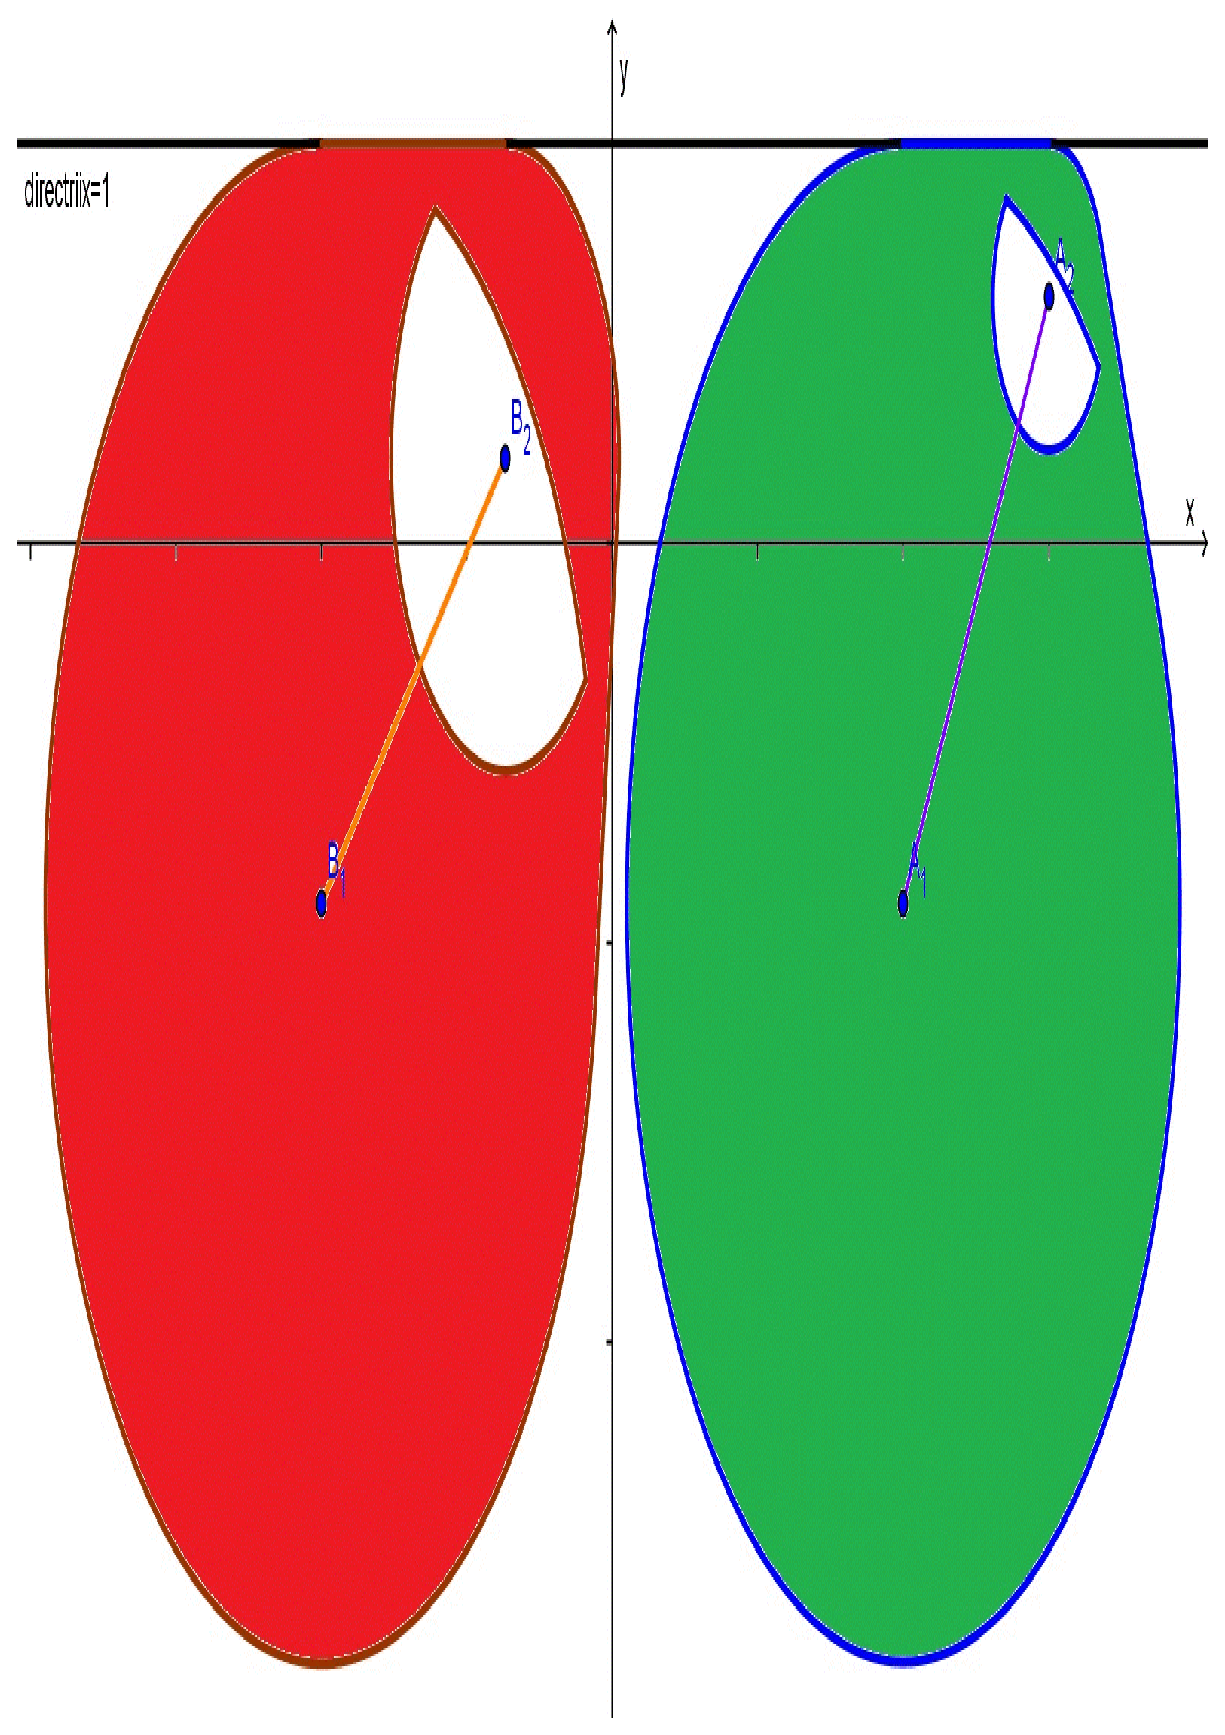
\includegraphics[width=100.5mm, height=52.2mm, viewport=3mm 4mm 205mm 292mm]{image6} а)\\
%%   \caption{}\label{image6}
%  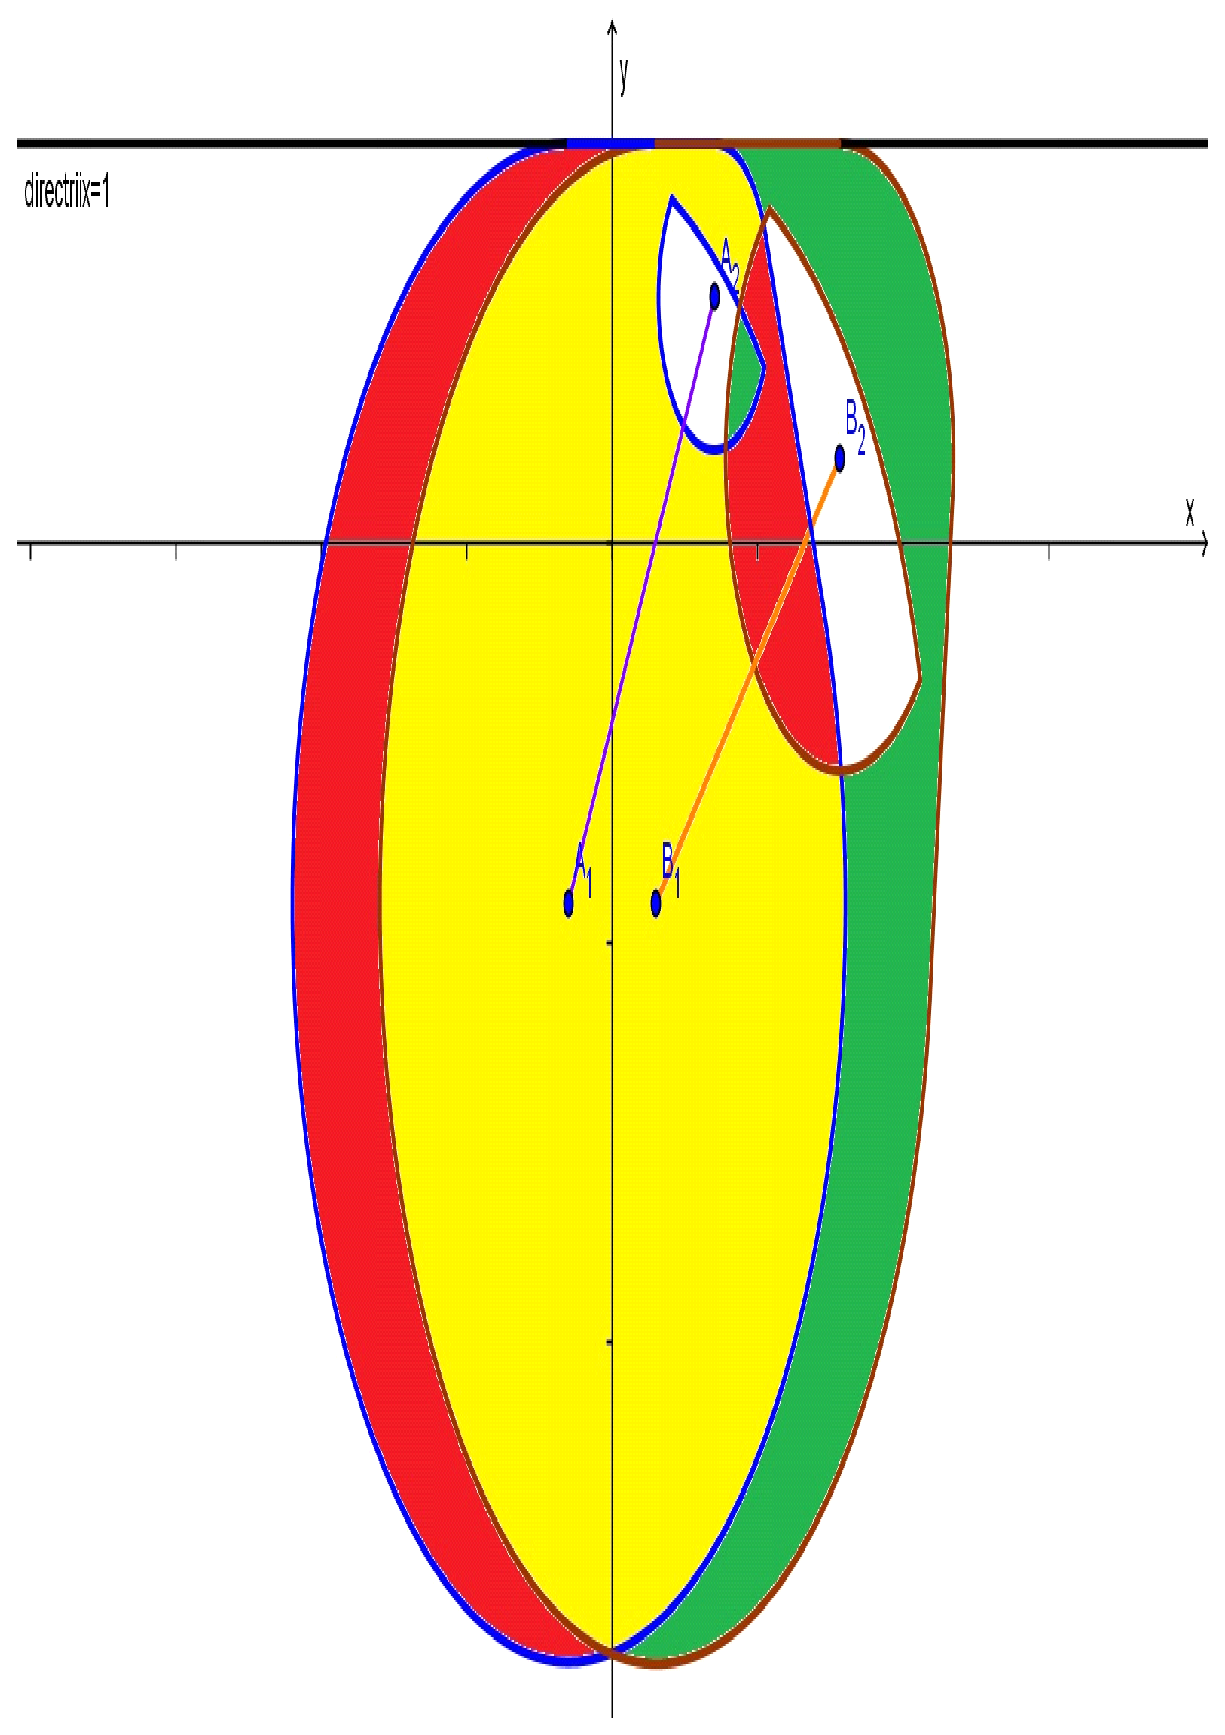
\includegraphics[width=100.5mm, height=52.2mm, viewport=3mm 4mm 205mm 292mm]{image7} б)\\
%  \caption{}\label{image6_7}
%\end{figure}
%
%Это означает, что в этой области $Q=A\cap B$ (на Рис.~\ref{image6_7}б обозначена желтым цветом) для любого фокуса существует сегмент параболы с концами, лежащими на \textit{разных} отрезках. Если же фокус не принадлежит $A-Q$ или $B-Q$, то конец любого сегмента траектории лежит на одном и том же отрезке. Подобные соображения могут быть распространены и на большее количество отрезков.

%Интересно отметить, что различные отношения отрезков, на которые разбивает данная точка «лакуны» зависит только от угла наклона $\alpha$
%
%\begin{equation} \label{GrindEQ__5_} \frac{A_{1} L}{LA_{2} } =\frac{1-y_{1} }{1-y_{2} } =\frac{2}{1-\sin \, \alpha } -1 , \frac{l_{2} }{A_{1} L} =\frac{2}{1+\sin \, \alpha }  \end{equation}
%
%Откуда можно найти значение угла $\alpha $, которому соответствует появление лакуны при золотом сечении отрезков. Т.е. из
%
%\[\frac{2}{1-\sin \, \alpha } -1=\frac{2}{1+\sin \, \alpha } =\varphi =\frac{1+\sqrt{5} }{2} , \sin \alpha =\sqrt{5} -2\]

Теперь перейдем собственно к фокусному отображению. Обозначим через $\bar{F}^{\pm } $ фокусы траекторий после отражения от точек $K^{\pm } $. Поскольку, как было показано ранее \cite{Yanovskii2013}, эти фокусы должны лежать на прямой, проходящей через $F$ под углом $2\alpha $, то отображение можно переписать следующим образом.

\begin{equation} \label{GrindEQ__6_} \bar{X}^{\pm } =X+t_{\pm } \cos \, 2\alpha ,  \bar{Y}^{\pm } =Y+t_{\pm } \sin \, 2\alpha  \end{equation}

И далее находим

\begin{equation} \label{GrindEQ__7_}t_{\pm } =\frac{2}{\cos \, \alpha } \left(\sigma \sqrt{\left(1-Y\right)d\left(X,Y,\alpha ,b\right)} -d\left(X,Y,\alpha ,b\right)\sin \, \alpha \right) \end{equation}

где $d\left(X,Y,\alpha ,b\right)$ то же расстояние от фокуса что и в \eqref{GrindEQ__2_}, $\sigma =\pm 1$ в определенном смысле задает направление «движения» фокуса в конфигурационном пространстве. Поскольку $\bar{F}^{\pm } $ также должно лежать на прямой параллельной $B1_{2} B2_{2} $, и она также наклонена на угол $2\alpha$ относительно оси $Ox$ , то ясно что $d\left(\bar{X},\bar{Y},\alpha ,b\right)=d\left(X,Y,\alpha ,b\right)$, как расстояние между параллельными прямыми. Учитывая это, можем перейти к новым координатам

\begin{equation} \label{GrindEQ__8_} \begin{array}{l} {\tilde{X}=1-b+\left(Y-b\right)\cos \, 2\alpha -X\sin \, 2\alpha ,} \\ {\tilde{Y}=1-Y} \end{array} \end{equation}

И подставляя в \eqref{GrindEQ__6_} и \eqref{GrindEQ__7_}, получим отображение

\begin{equation} \label{GrindEQ__9_} \begin{array}{l} {\bar{\tilde{X}}=\tilde{X},} \\ {\bar{\tilde{Y}}=f^{\sigma } \left(\tilde{X},\tilde{Y}\right)=\tilde{Y}-4\tilde{X}\sin ^{2} \alpha \left(\frac{\sigma }{\sin \, \alpha } \sqrt{\frac{\tilde{Y}}{\tilde{X}} } -1\right)} \end{array} \end{equation}

Но само по себе оно не является полным, пока мы не записали отображение для  $\bar{\sigma }\left(\sigma ,\tilde{X},\tilde{Y}\right)$. Здесь нам поможет условие обратимости траектории частицы по времени. Ясно, что общий вид \eqref{GrindEQ__9_} должен оставаться верным если заменить $\tilde{Y}\leftrightarrow \bar{\tilde{Y}},\tilde{X}\leftrightarrow \bar{\tilde{X}}$. Существуют четыре возможных комбинации $\left(\sigma ,\bar{\sigma }\right)$для которых. $f^{\sigma } \circ f^{\bar{\sigma }} =1$. Однако из них могут реализоваться только следующие: $f^{\pm } \circ f^{\mp } =1$ и $f^{+} \circ f^{+} =1$. Это легко видно из графиков для $f^{\pm } $, представляющих собой совместно параболу (Рис.2). Ветвь$f^{-} $-- строго возрастающая функция, с началом в точке $B$, а поэтому $f^{-} \circ f^{-} =1$ невозможно. На Рис.2 видно, что единственный участок убывания имеет ветвь $f^{+} $на участке $\tilde{Y}\in \left(0,4\tilde{X}\sin ^{2} \, \alpha \right)$(т.е. между точками $A$ и $B$). Только на этом участке возможно отображение $f^{+} \circ f^{+} =1$.

%\begin{figure}[ht]
%  \centering
%  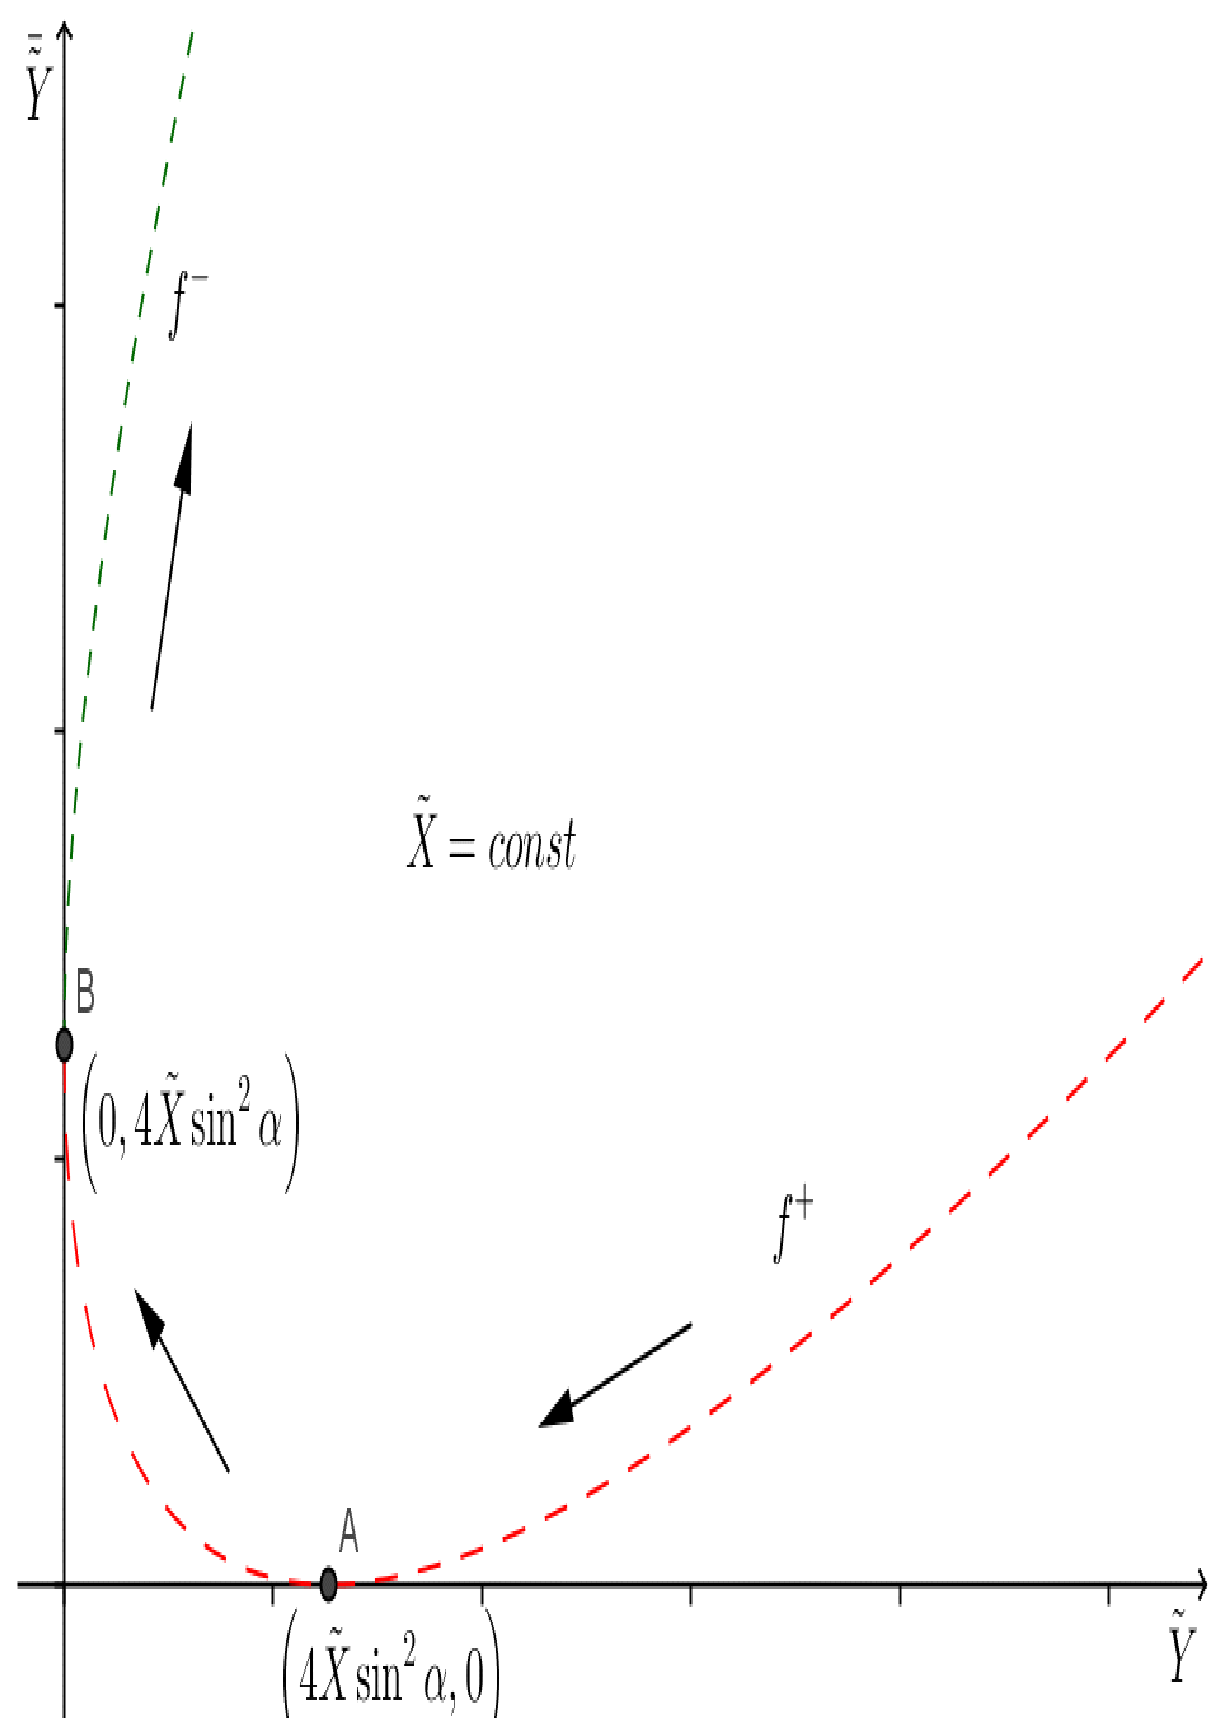
\includegraphics[width=96.8mm, height=67.7mm, viewport=3mm 4mm 205mm 292mm]{image8}\\
%  \caption{}\label{image8}
%\end{figure}

\begin{figure}[h]
\center{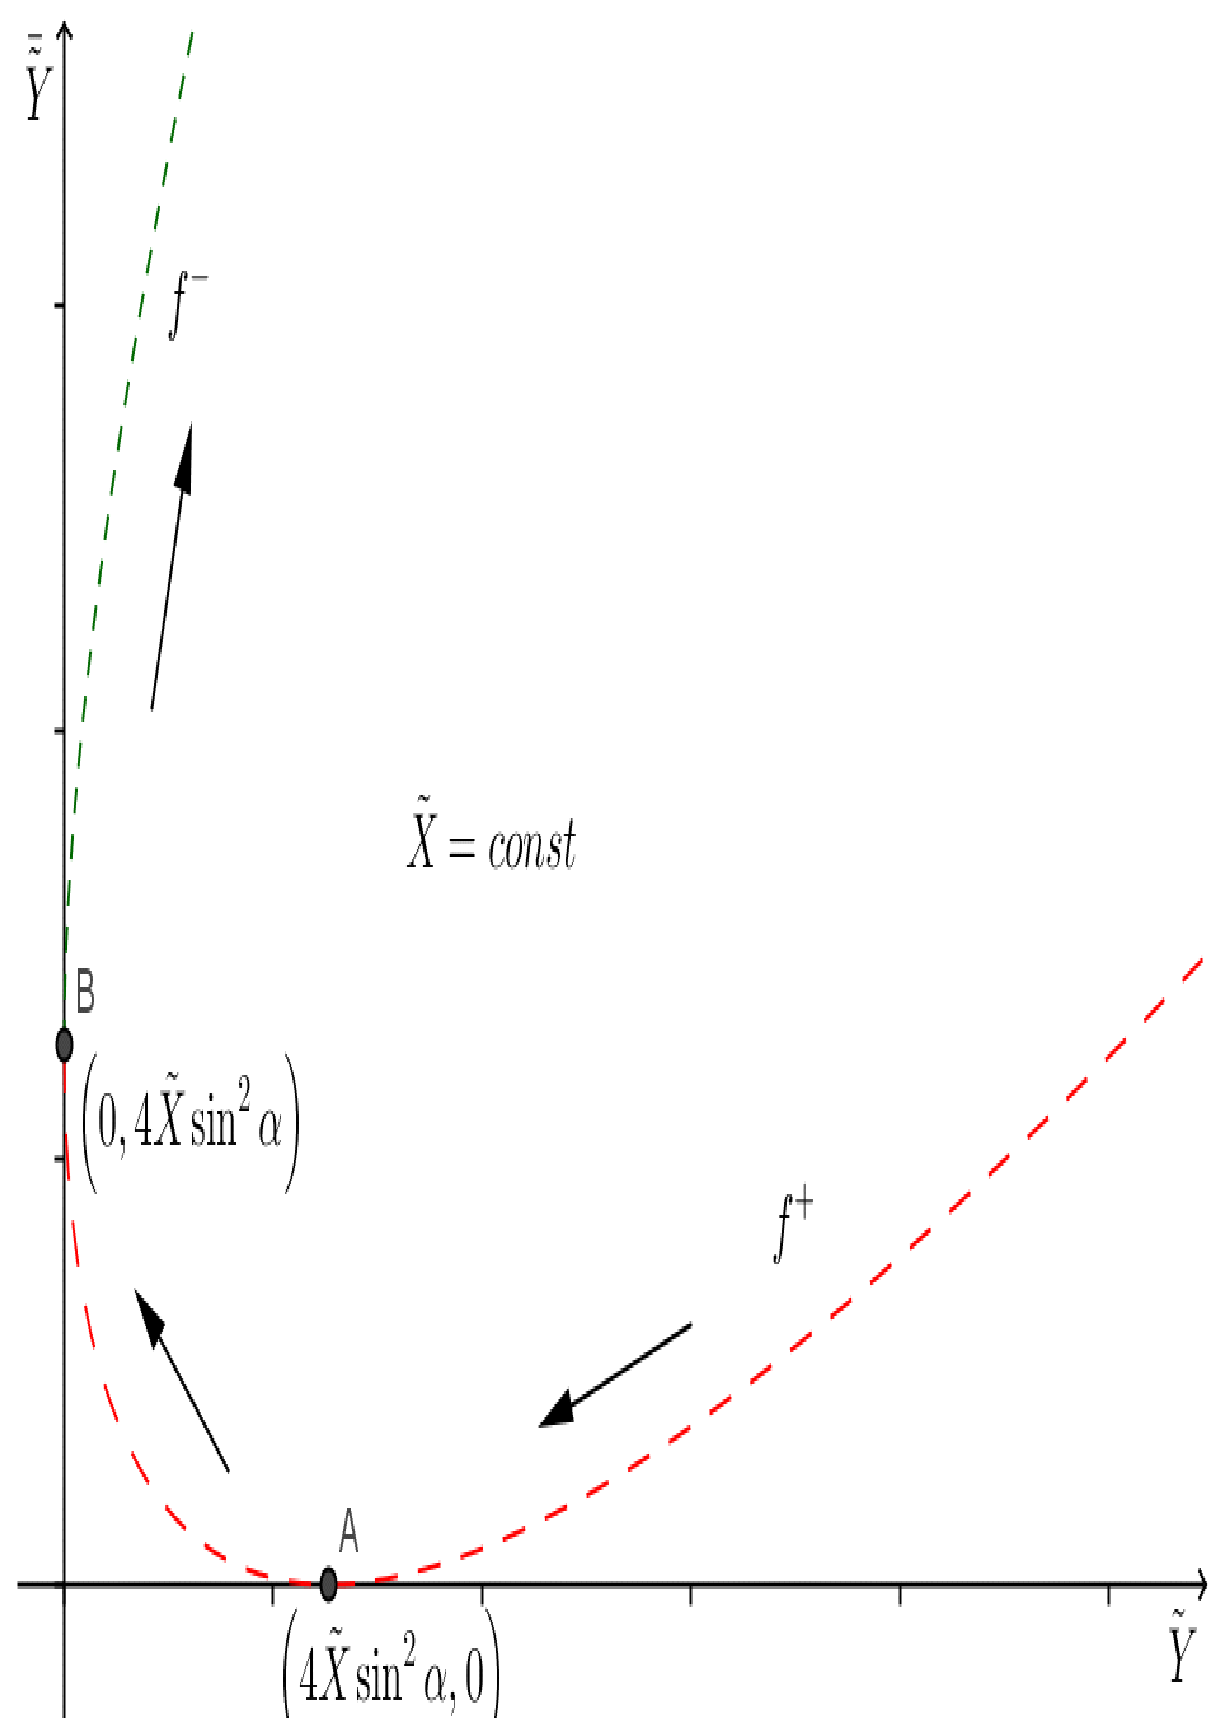
\includegraphics[width=.5\linewidth]{image8}}
\caption{ Показана траектория и ее направление для отображения \eqref{GrindEQ__9_} }
\label{image8}
\end{figure}

Траектория частицы на наклонной стороне не имеет зацикливаний (здесь мы предполагаем, что частица падает сверху на стенку). Поэтому, если мы возьмем в качестве начальной ветвь $f^{-} $ , то при дальнейшей эволюции ее знак уже не меняется (иначе было бы зацикливание). Для $f^{+} $ситуация несколько иная. На участке $\tilde{Y}>4d\sin ^{2} \, \alpha $ при эволюции, по той же причине, что и выше, мы также должны брать $f^{+} $. Поскольку, при этом будет выполняться условие $\bar{\tilde{Y}}<\tilde{Y}$, то в какой-то момент выполнится условие $\bar{\tilde{Y}}_{n} \le 4d\sin ^{2} \, \alpha $. И если мы не изменим знак отображения, то произойдет указанное раннее зацикливание $f^{+} \circ f^{+} =1$, чего не должно быть. Поэтому далее мы должны изменить знак отображения и его эволюция пойдет по предыдущему «минусовому» сценарию. Иными словами, эволюция траектории всегда идет в направлении стрелок как показано на Рис.\ref{image8}.

Парабола, состоящая из ветвей $f^{\pm } $ может быть параметризована следующим образом.

\begin{equation} \label{GrindEQ__10_} \begin{array}{l} {\tilde{Y}=\frac{\left(4\tilde{X}\sin \alpha +\tau \csc \alpha \right)^{2} }{16\tilde{X}} ,} \\ {\bar{\tilde{Y}}=\frac{\left(4\tilde{X}\sin \alpha -\tau \csc \alpha \right)^{2} }{16\tilde{X}} } \end{array} \end{equation}

В этом случае $\tau $ соответствует двум сопряженным значениям $\left(\tilde{Y},\bar{\tilde{Y}}\right)$. Соответственно, $\bar{\tau }$ должно соответствовать значениям$\left(\bar{\tilde{Y}},\bar{\bar{\tilde{Y}}}\right)$, т.к. конец одного сегмента траектории соответствует началу следующего. Поэтому из

\begin{equation} \label{GrindEQ__10_1_} \bar{\tilde{Y}}=\frac{\left(4\tilde{X}\sin \alpha +\bar{\tau }\csc \alpha \right)^{2} }{16\tilde{X}} =\frac{\left(4\tilde{X}\sin \alpha -\tau \csc \alpha \right)^{2} }{16\tilde{X}}  \end{equation}

получаем

\begin{equation} \label{GrindEQ__11_} \bar{\tau }=\tau -8\tilde{X}\sin ^{2} \alpha  \end{equation}

Переходя теперь к переменным $\left(\tilde{X},\tau \right)$,  мы получаем не только очень простое линейное отображение, но и избавляемся от неоднозначности, которая нам мешала в «чисто» фокусном отображении \eqref{GrindEQ__7_} (имеется в виду $\sigma$).

Кроме того, из \eqref{GrindEQ__10_} мы можем выразить $\tau $ через $t$

\begin{equation} \label{GrindEQ__11_1_} \tau _{\pm } =4\tilde{X}\sin \alpha \left(\pm \sqrt{\frac{\tilde{Y}}{\tilde{X}} } -\sin \alpha \right)=t_{\pm } \sin 2\alpha  \end{equation}

Где $t_{\pm } $ -- это расстояние между фокусами из \eqref{GrindEQ__7_}. Таким образом, $\tau $ имеет простой геометрический смысл -- это изменение $y$-координаты фокуса сегмента траектории при отражении от стенки

\begin{equation} \label{GrindEQ__11_2_} \tau =\Delta Y=\bar{Y}-Y \end{equation}

Дополнительно можно  отметить, что разделив обе части уравнения \eqref{GrindEQ__9_} на $d=4\tilde{X}\sin ^{2} \alpha $ и сделав замену $\nu =\frac{\tilde{Y}}{4\tilde{X}\sin ^{2} \alpha } $ получим безразмерное отображение для $\nu $, не зависящее от угла наклона $\alpha $

\begin{equation} \label{GrindEQ__11_2_1_}\bar{d}=d,\; \bar{\nu }=\nu \pm 2\sqrt{\nu } +1 \end{equation}

%\begin{figure}[ht]
%  \centering
%  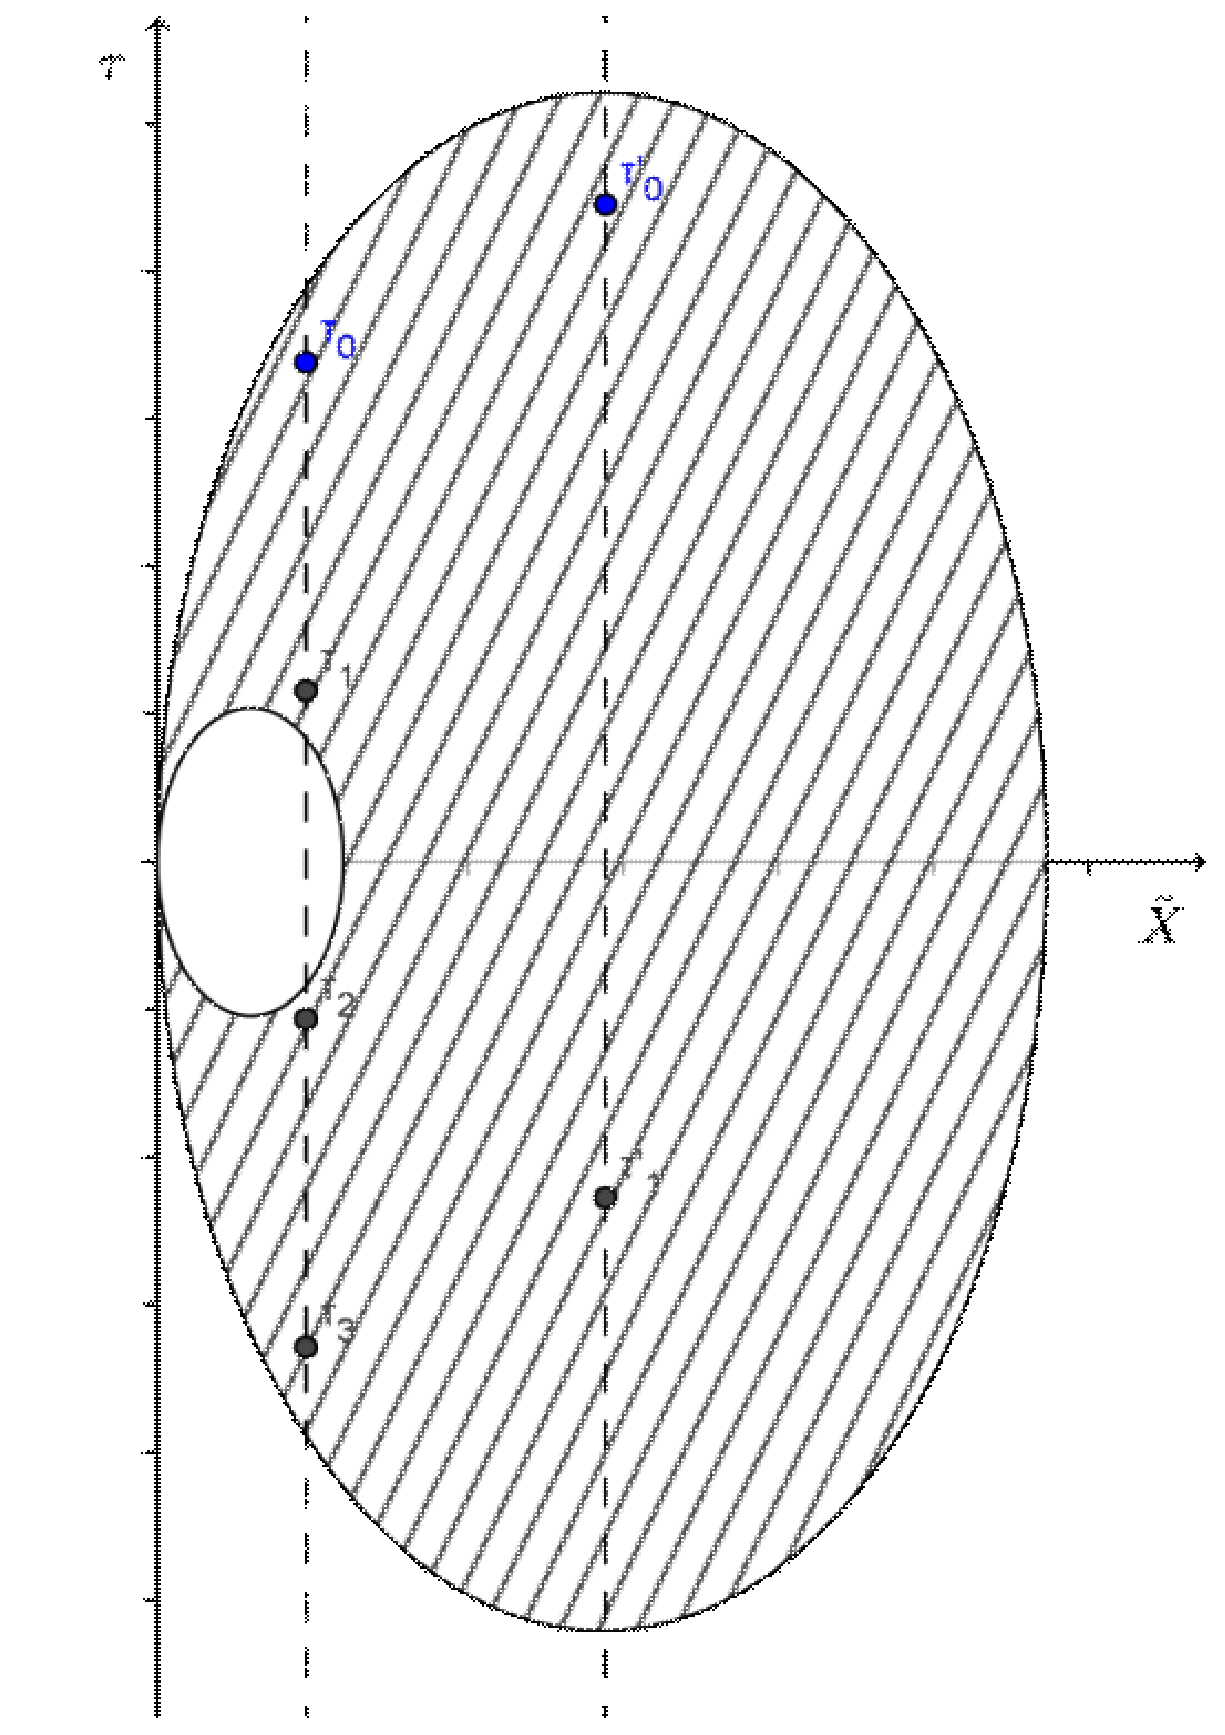
\includegraphics[width=71.2mm, height=106.7mm, viewport=3mm 4mm 205mm 292mm]{image9.eps}\\
%  \caption{Представлены две типичные траектории отображения \eqref{GrindEQ__11_}.}\label{image9}
%\end{figure}

% 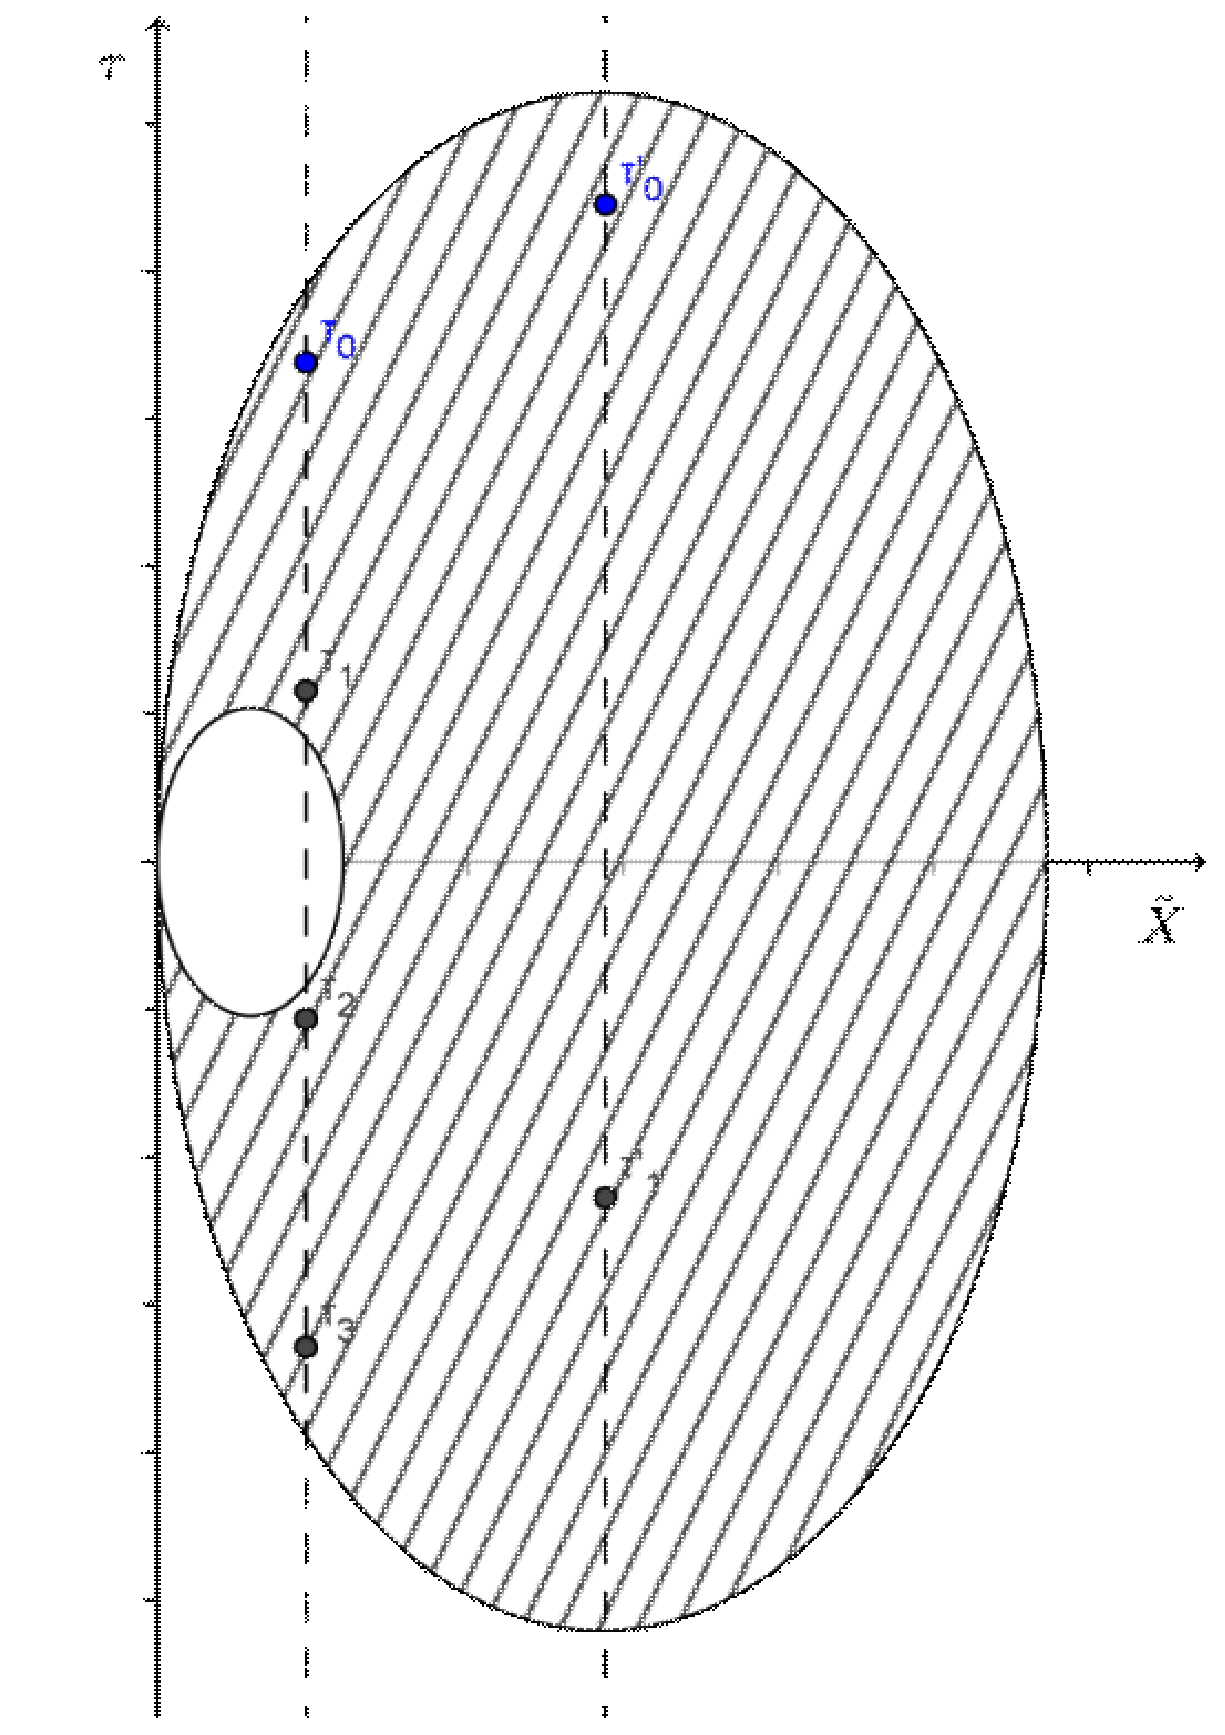
\includegraphics[width=71.2mm, height=106.7mm, viewport=3mm 4mm 205mm 292mm]{image9}
Это отображение также параметризуется, поскольку в неявном виде также представляет собой параболу. Теперь \eqref{GrindEQ__10_} можно переписать как

\begin{equation} \label{GrindEQ__11_2_2_}\nu =\frac{\left(1+\tau '\right)^{2} }{4} ,\bar{\nu }=\frac{\left(1-\tau '\right)^{2} }{4} \end{equation}

А отображение \eqref{GrindEQ__11_} переходит в

\begin{equation} \label{GrindEQ__11_2_3_}\bar{\tau }'=\tau '-2 \end{equation}
и далее
\begin{equation} \label{GrindEQ__11_2_4_} d=4\tilde{X}\sin ^{2} \alpha ,\; \quad \tau '=\frac{\tau }{d} =\frac{\tau }{4\tilde{X}\sin ^{2} \alpha } ,\quad \nu =\frac{1-Y}{d} =\frac{\tilde{Y}}{4\tilde{X}\sin ^{2} \alpha } \end{equation}

 Выше мы рассматривали отображение для бесконечной стенки. Теперь вернемся к отрезку и рассмотрим уже в новых координатах $\left(\tilde{X},\tau \right)$ область определения данного отображения. Воспользуемся выражением \eqref{GrindEQ__2_} для $l_{\pm } $. Для сегментов траекторий попадающих на конец отрезка должно выполняться условие $l_{\pm } =0$. Выражая теперь $\left(X,Y\right)$ через $\left(\tilde{X},\tau \right)$ получим выражение

\begin{equation} \label{GrindEQ__12_} \tau _{i} =\pm 2\sin 2\alpha \sqrt{\tilde{X}\left(2\left(1-b-x_{i} tg\, \alpha \right)-\tilde{X}\right)} =\pm 2\sin 2\alpha \sqrt{\tilde{X}\left(2\left(1-y_{i} \right)-\tilde{X}\right)}  \end{equation}

где $i=1,2$ нумерует концы отрезка $A_{i} $ (см. Рис.~\ref{image5}). Соответственно, $\tau _{i} $ -- это такие значения параметра, при котором парабола пройдет через точки $A_{i} $. Переписывая \eqref{GrindEQ__12_} в неявном виде

\begin{equation} \label{GrindEQ__13_} \frac{1}{\left(1-y_{i} \right)^{2} } \left(\frac{\tau ^{2} }{4\sin ^{2} 2\alpha } +\left(\tilde{X}-\left(1-y_{i} \right)\right)^{2} \right)=1 \end{equation}

Gолучим уравнение эллипса. 
% как показано на Рис.~\ref{image9}. 
Таким образом, область определения представляет собой внутреннюю область эллипса исключая эллиптическую лакуну. Лакуна соответствует точке отрезка \textit{i} с большей $y$ координатой. Если какой либо из $y_{i} \ge 1$, то лакуна исчезает (в уравнение \eqref{GrindEQ__13_} тогда нужно подставить $y_{i} \to 1$).

\section{ Отображение в наклонном клине}

Вернемся к Рис.\ref{fig:in1} и построим теперь отображение в наклонном клине (наклонным клином назовем клин, в котором выполняются условия $0<\alpha <\beta <{\raise0.7ex\hbox{$ \pi  $}\!\mathord{\left/ {\vphantom {\pi  2}} \right. \kern-\nulldelimiterspace}\!\lower0.7ex\hbox{$ 2 $}} $ или область \textit{u-d/fin} на Рис. \ref{fig:angle_diagram}). В этом случае мы также можем применить фокусный подход аналогичный тому, который мы использовали при исследовании отражения от наклонной стенки.

\begin{figure}[h]
\center{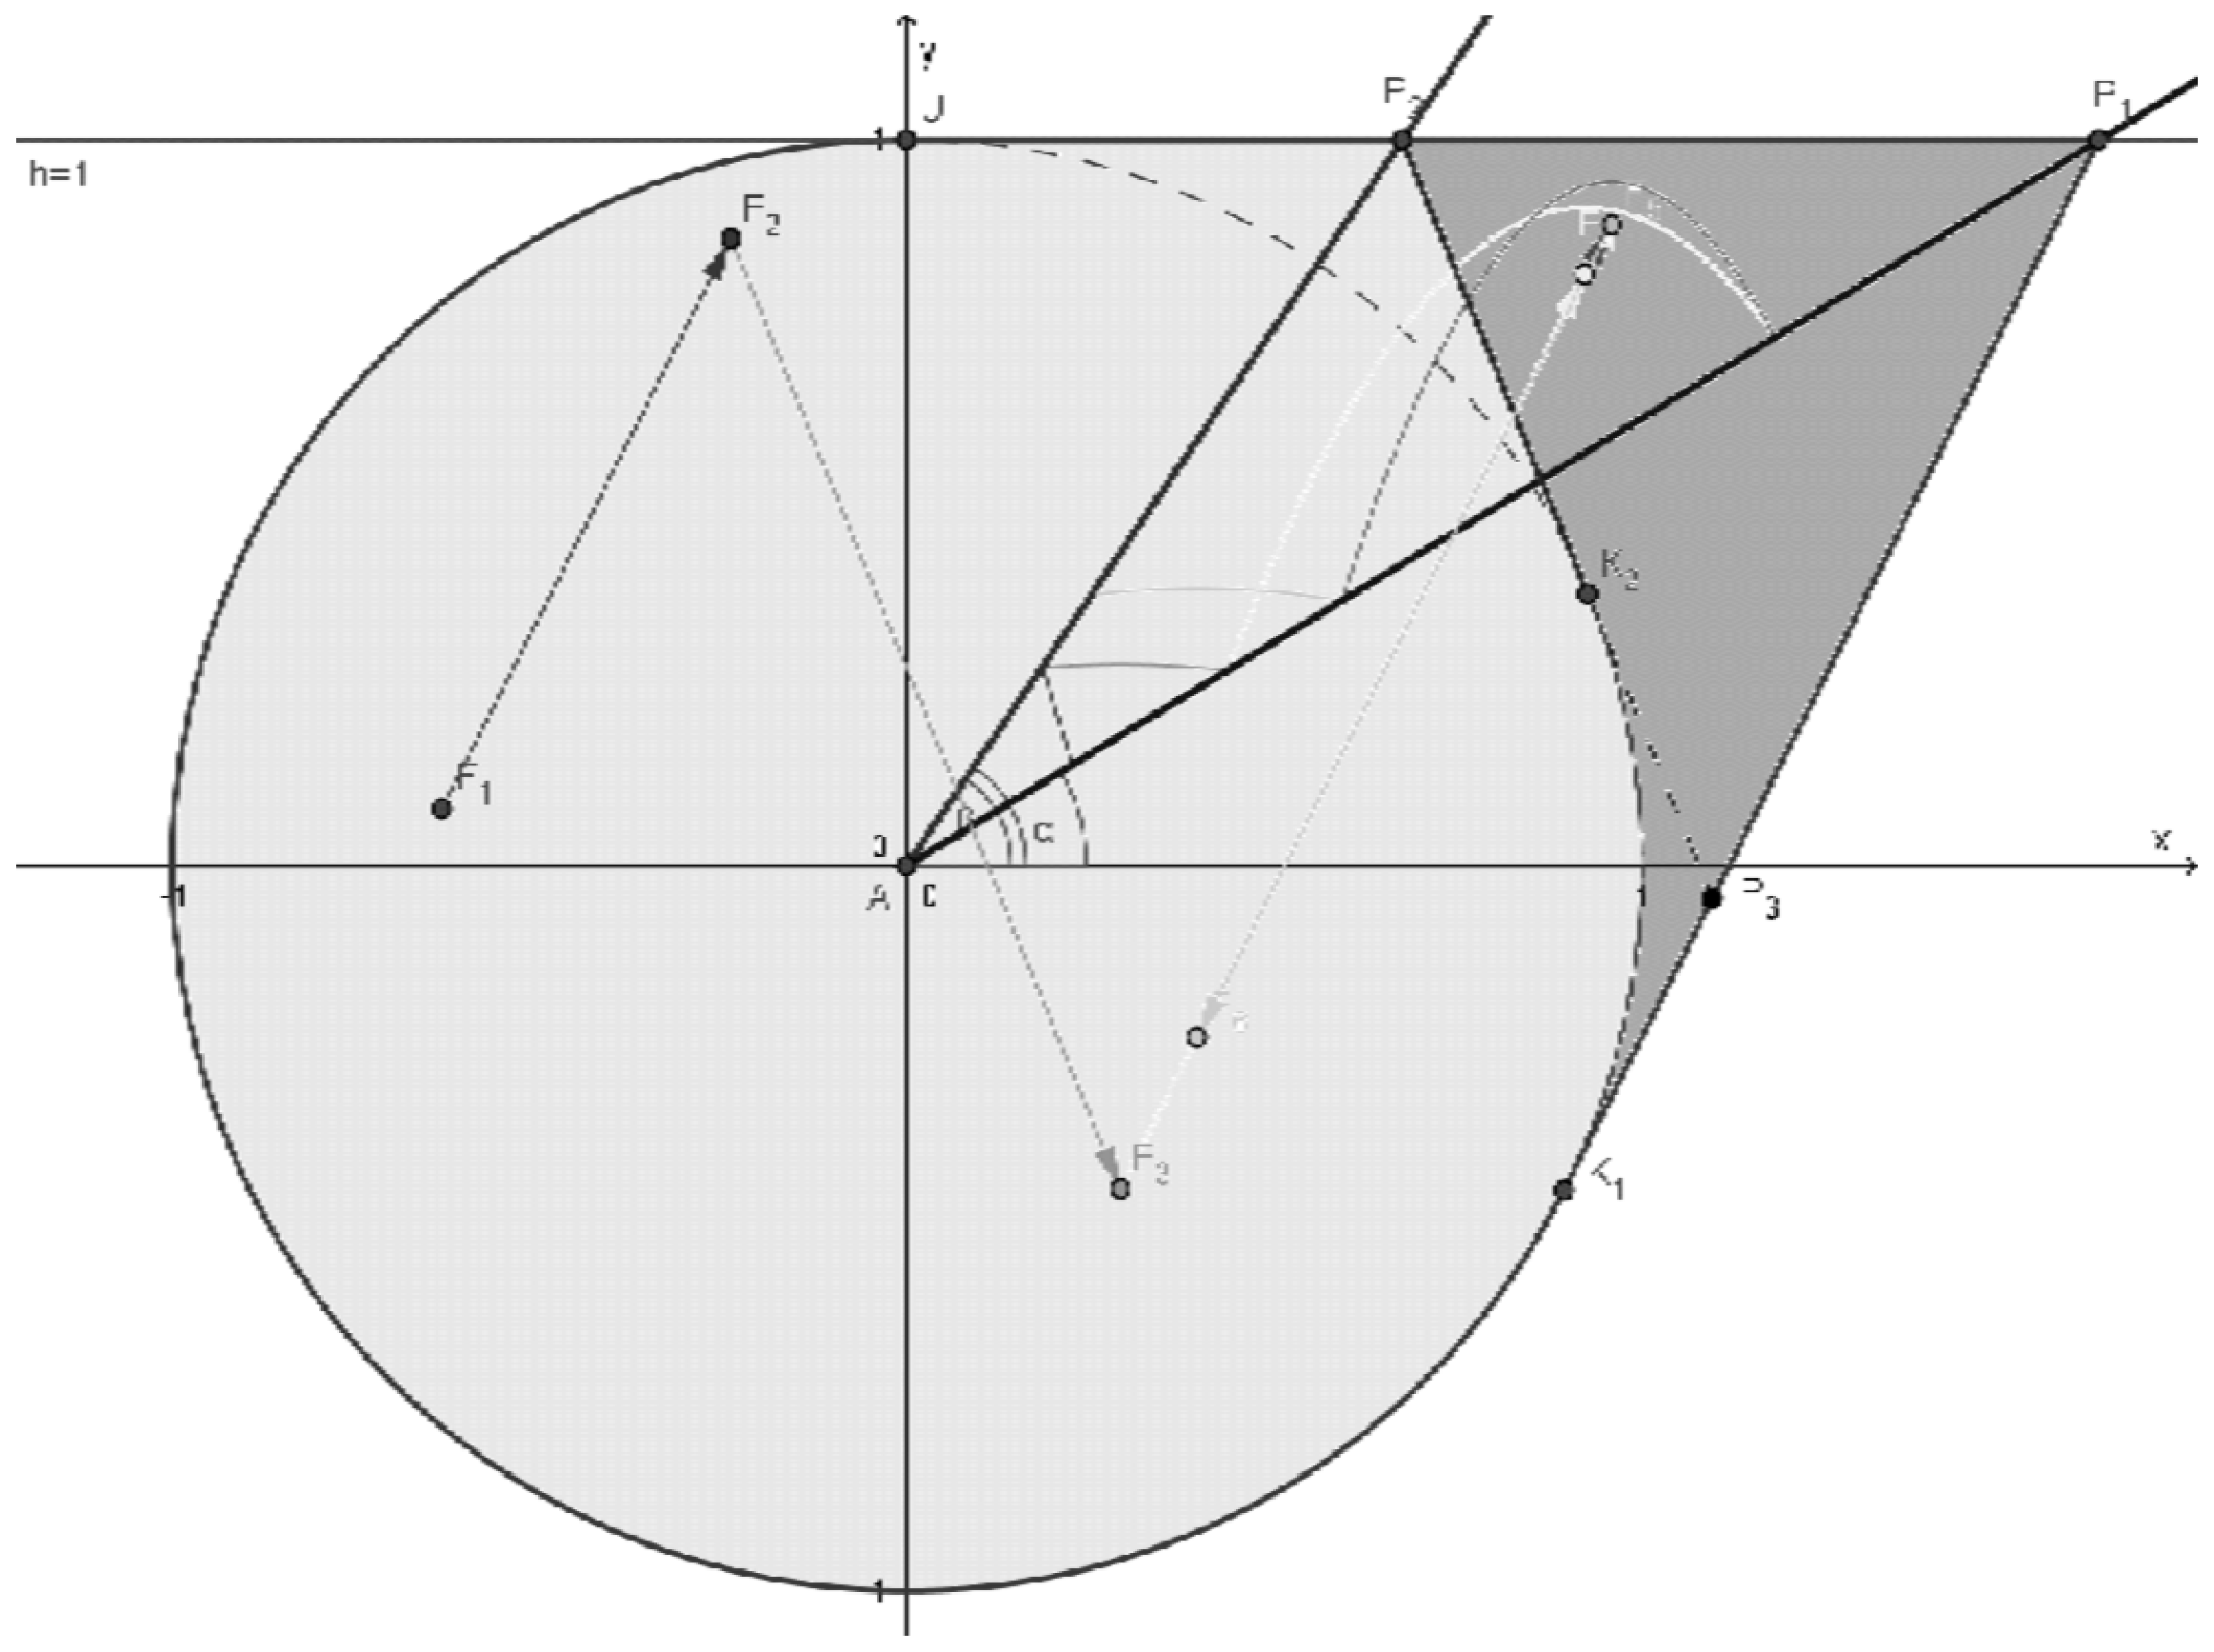
\includegraphics[width=0.5\linewidth]{image10}}
\caption{Показано соответствие нескольких сегментов траектории в клине с точками фокусного отображения для наклонного клина. }
\label{image10}
\end{figure}

%\begin{figure}[ht]
%  \centering
%  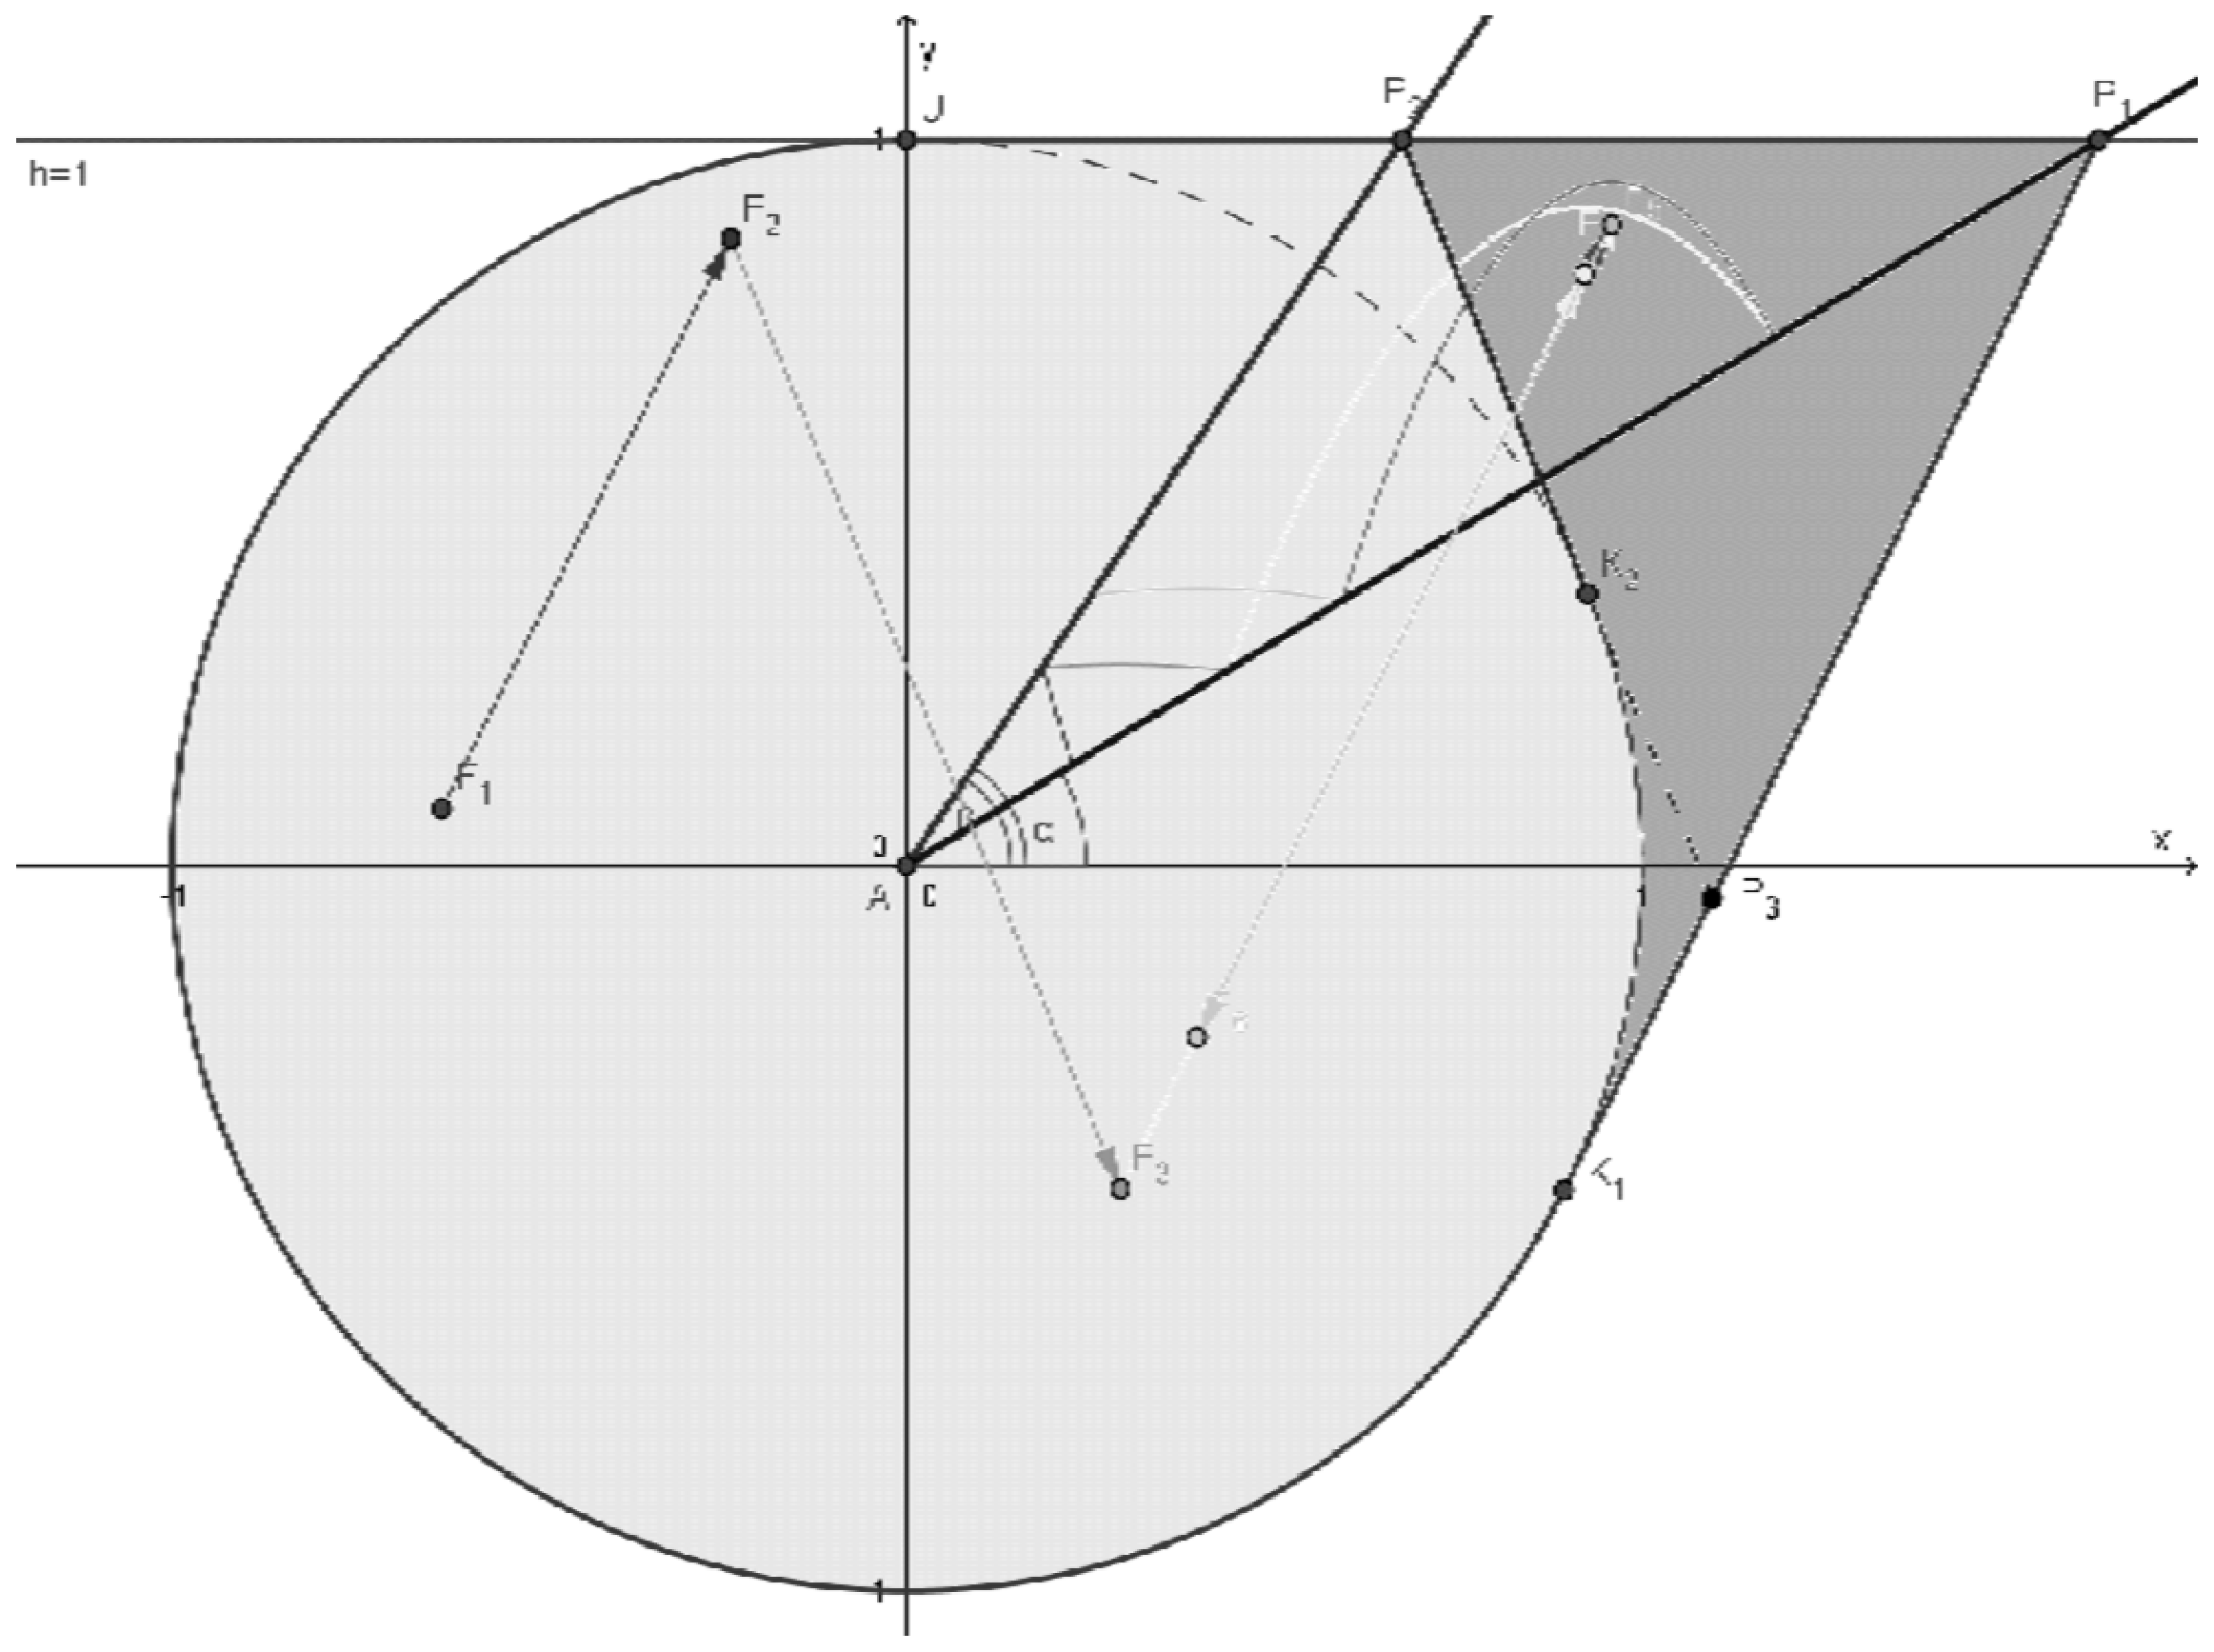
\includegraphics[width=123.3mm, height=88.8mm, viewport=3mm 4mm 205mm 292mm]{image10}\\
%  \caption{}\label{image10}
%\end{figure}

Ясно, что отображение \eqref{GrindEQ__9_} 
%или \eqref{GrindEQ__11_2_1_} 
 применимы при каждом отражении от соответствующей наклонной стенки клина. При этом добавляется еще один параметр -- текущий номер (или угол) стенки. Тогда в общем виде отображение будет формально 3-мерным с дополнительным дискретным параметром $i$ -- номером стенки (не путать с $i$ для концов отрезка в предыдущем разделе). В общем виде это отображение можно записать так:

\begin{equation} \label{GrindEQ__20_}
 \begin{array}{l}
  {\bar{i}=i_{+} \left(d,\tau ,i\right),} \\ {\bar{d}=d_{+} \left(d,\tau ,i,\bar{i}\right),} \\ {\bar{\tau }=\tau _{+} \left(d,\tau ,i,\bar{i}\right),}
   \end{array}
    \end{equation}

Здесь «$+$» в нижнем индексе означает функцию отображение соответствующего переменной, $d =\tilde{X} $ и $\tau '=\frac{\tau }{2 \sin (2 \alpha )}$ (для краткости здесь и далее мы будем опускать штрих при $\tau$), а $\alpha _{i} $ -- соответствующие углы стенок (в данном случае и в дальнейшем $\alpha _{1} =\alpha$, $\alpha _{2} =\beta $ на Рис.\ref{image4} и Рис.\ref{image10}).
Из \eqref{GrindEQ__13_} мы можем получить неявное уравнение в этих переменных для семейства всех траекторий, падающих на наклонную стенку в точку на высоте $y$.

\begin{equation} \label{GrindEQ__21_4} R\left(d,\tau,y\right)=(1-y-d)^2+\tau ^2-(1-y)^2=0 \end{equation}
Здесь и далее мы подразумеваем одинаковые индексы для $\tau$, $d$ и $y$ если они не указаны явно. 

Откуда находим область определения для клина

 \begin{equation} \label{GrindEQ__21_5} R\left(d,\tau,0\right)<0 \end{equation}


%\begin{equation} \label{GrindEQ__21_} R\left(d ,\tau _{i} ,\alpha _{i} ,b\right)=\frac{\tau _{i} ^{2} d_{i} ^{2} }{4\left(1-b\right)^{2} \sin ^{2} 2\alpha _{i} } +\left(\frac{d_{i} }{4\left(1-b\right) \sin ^{2} \alpha _{i} } -1\right)^{2} <1 \end{equation}

%\begin{equation} \label{GrindEQ__21_} R\left(d,\tau\right)=(d-1)^2+\tau ^2<1 \end{equation}

Т.е. круг единичного радиуса с центром в точке $(1,0)$ (см. Рис. \ref{fig:phaseAB}) не зависящий от угла наклона, что представляет определенные удобства для исследования. 
% Слева обе области ограничены прямой $d=0$, а справа кривыми соответствующих цветов. Синий -- это для первой, «нижней» стенки, а голубой -- для второй, «верхней» стенки.
%\begin{figure}[ht]
%  \centering
%  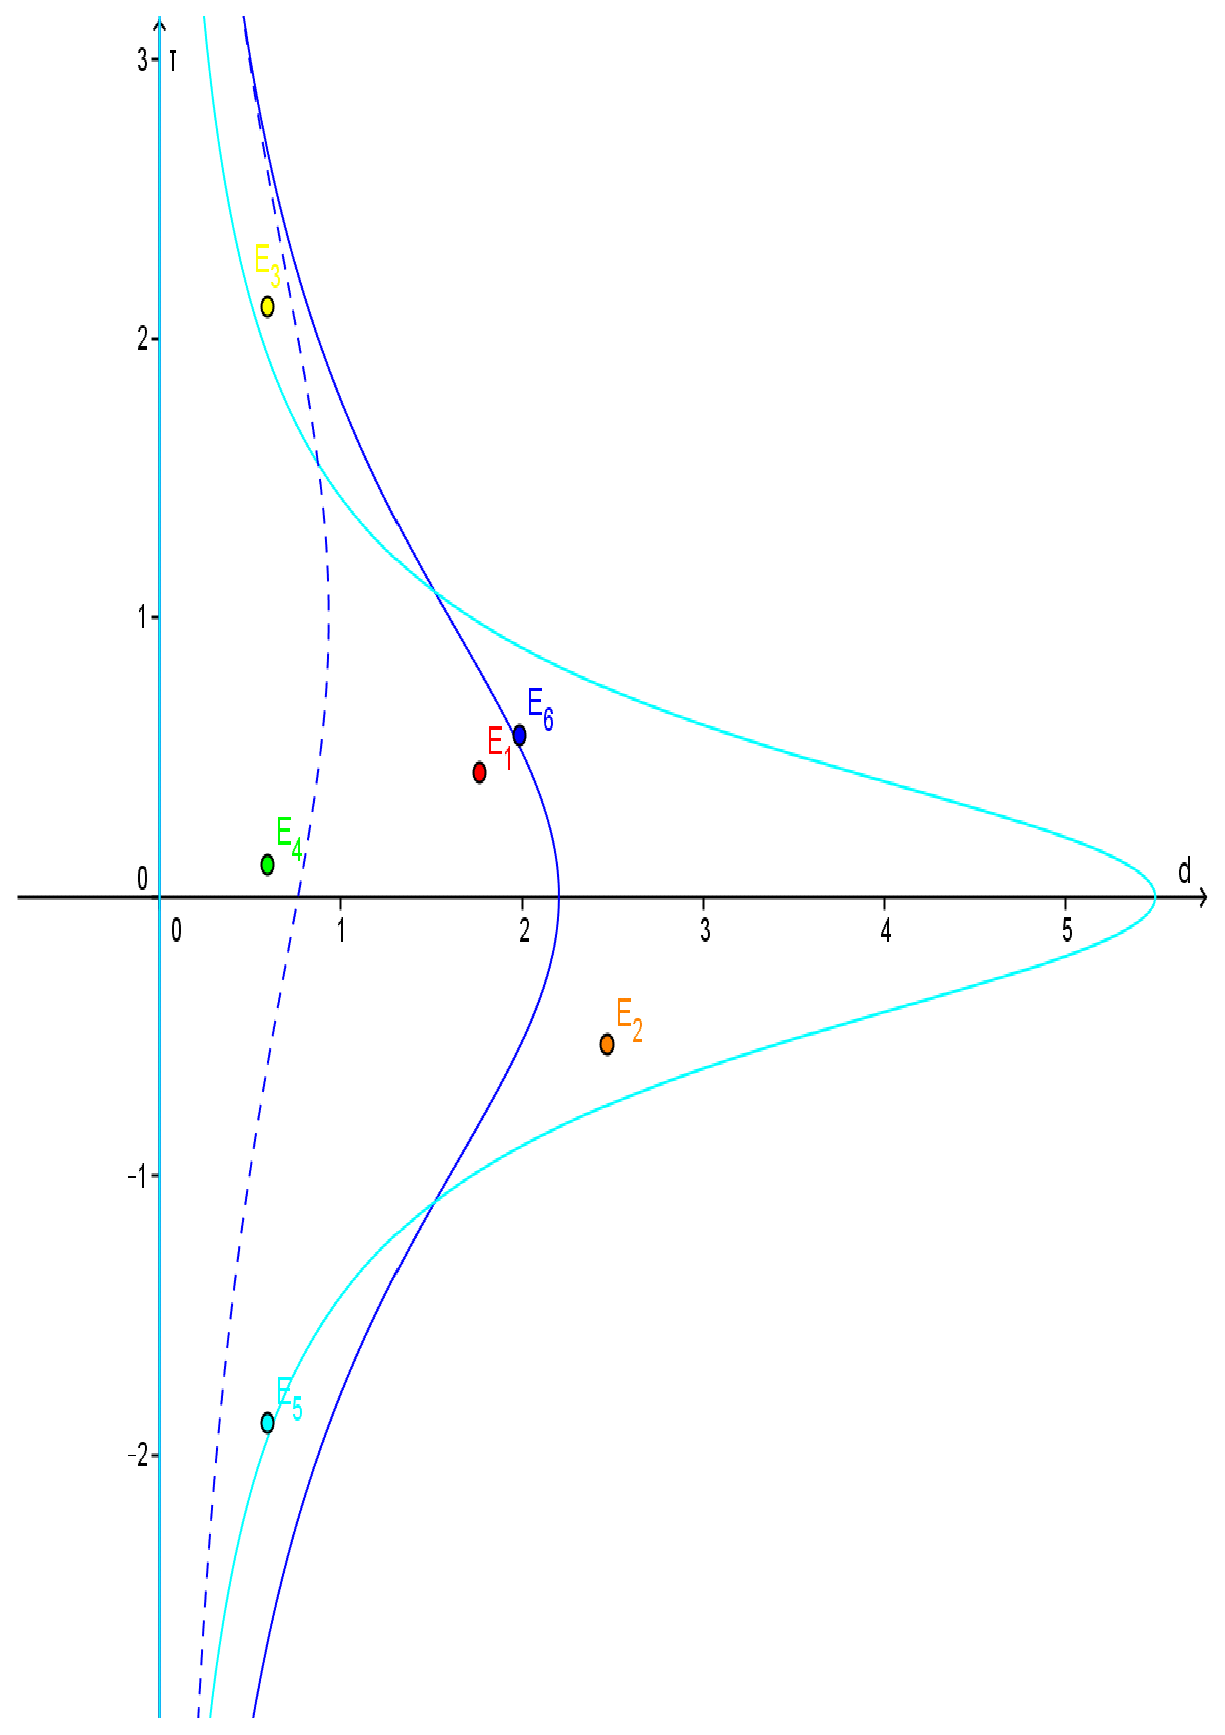
\includegraphics[width=91.0mm, height=80.7mm, viewport=3mm 4mm 205mm 292mm]{image11}\\
%  \caption{}\label{image11}
%\end{figure}

%\begin{figure}[h]
%\begin{minipage}[h]{0.49\linewidth}
%\center{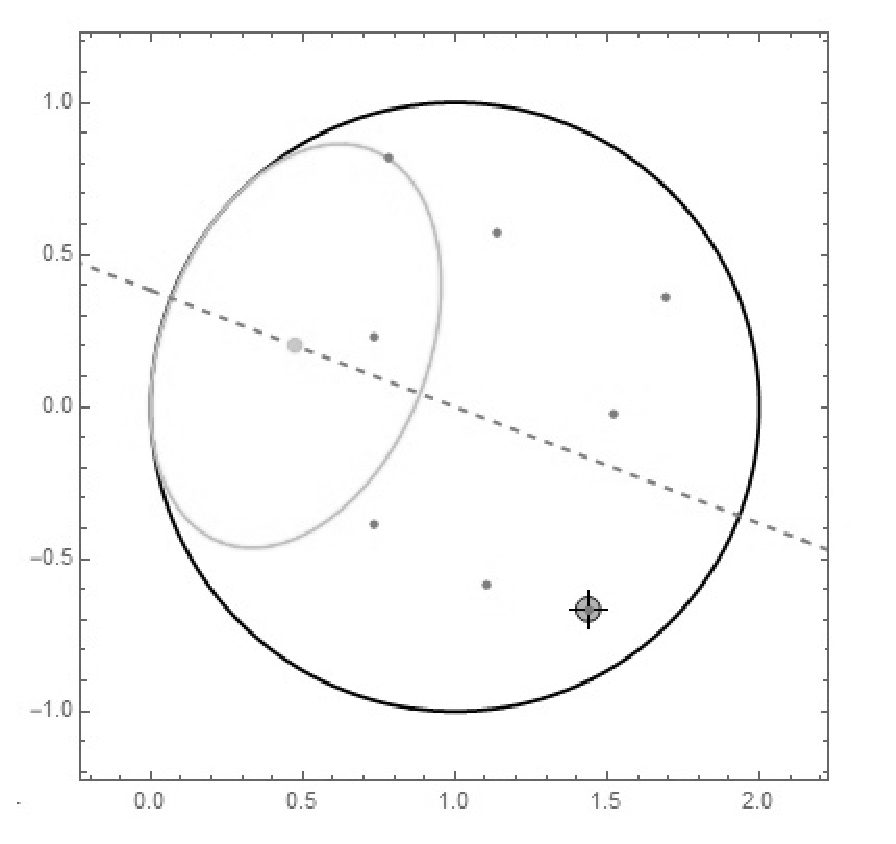
\includegraphics[width=.7\linewidth]{phaseA} \\ а)}
%\end{minipage}
%\hfill
%\begin{minipage}[h]{0.49\linewidth}
%\center{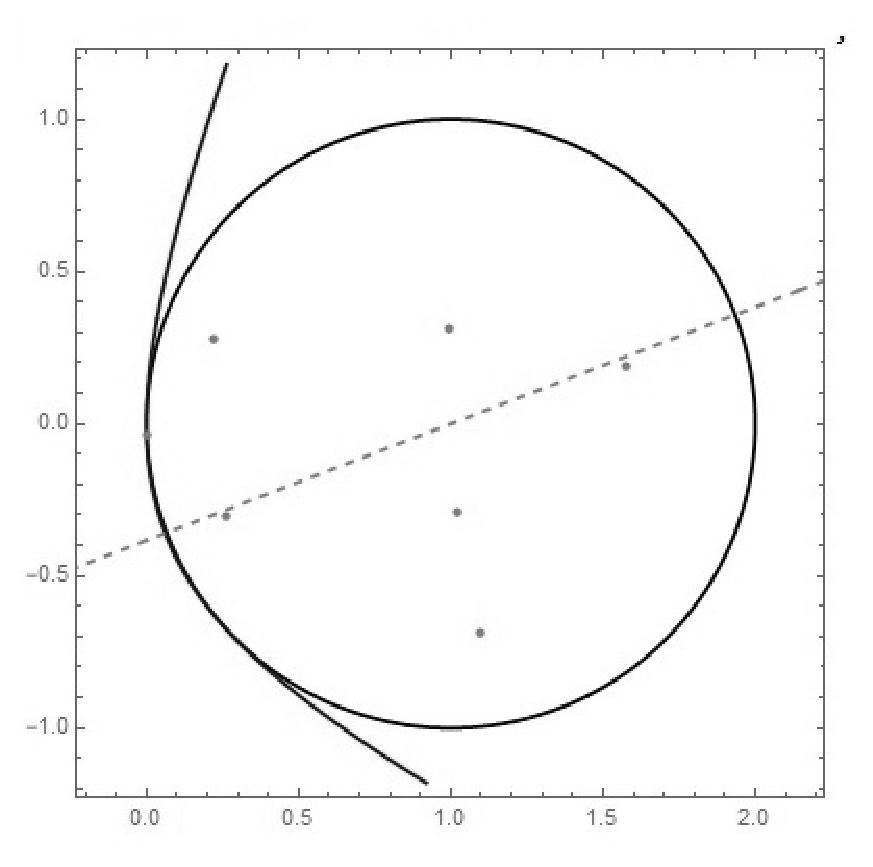
\includegraphics[width=.7\linewidth]{phaseB} \\ б)}
%\end{minipage}
%\caption{Несколько точек фазового портрета для клина, изображенного на Рис. \ref{image10} с указанием области соответствующих квадратичных форм из \eqref{EQ_quadratic}. Рис. (а) соответствует нижней стороне клина, а (б) соответственно верхней. Легко заметить, что на левом рисунке если точка попадает в область эллипса, то далее обязательно попадает на ту же сторону с неизменным значением $d$. Пунктиром обозначены главные оси квадратичных форм}.  
%\label{phaseAB}
%\end{figure}

\begin{figure}[h!]
  \centering
  \begin{subfigure}[b]{0.4\linewidth}
    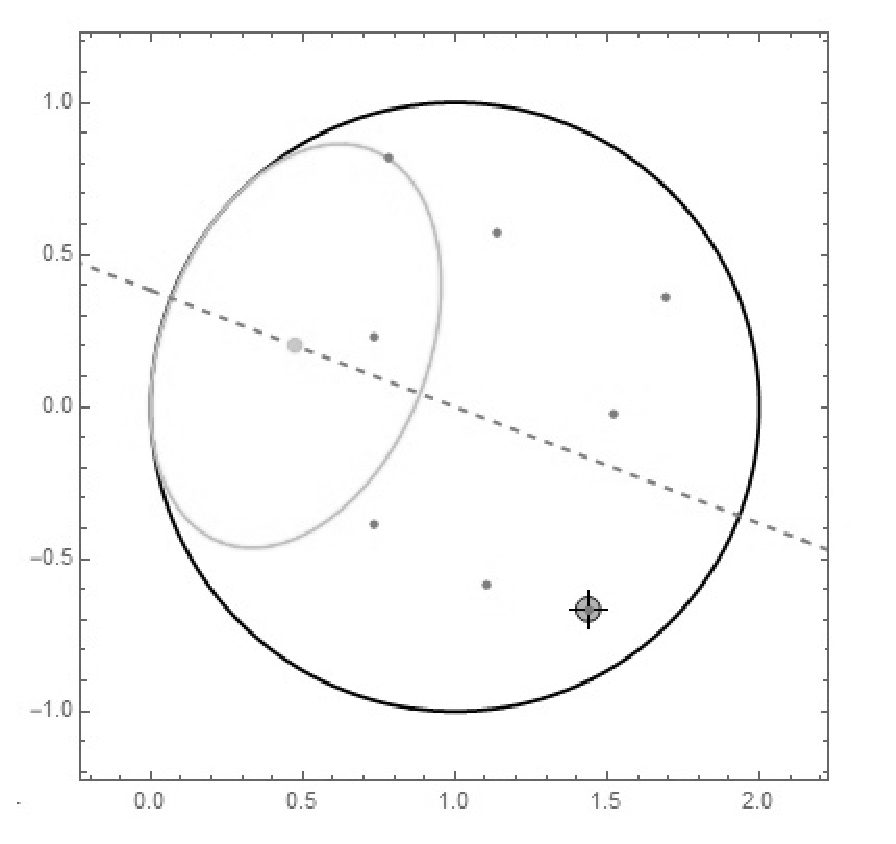
\includegraphics[width=\linewidth]{phaseA}
    \caption{Соответствует нижней стороне клина. Если точка попадает в область эллипса, то далее обязательно попадает на ту же сторону с неизменным значением $d$.}
    \label{fig:phaseA}
  \end{subfigure}
  \quad\quad\quad\quad
  \begin{subfigure}[b]{0.4\linewidth}
    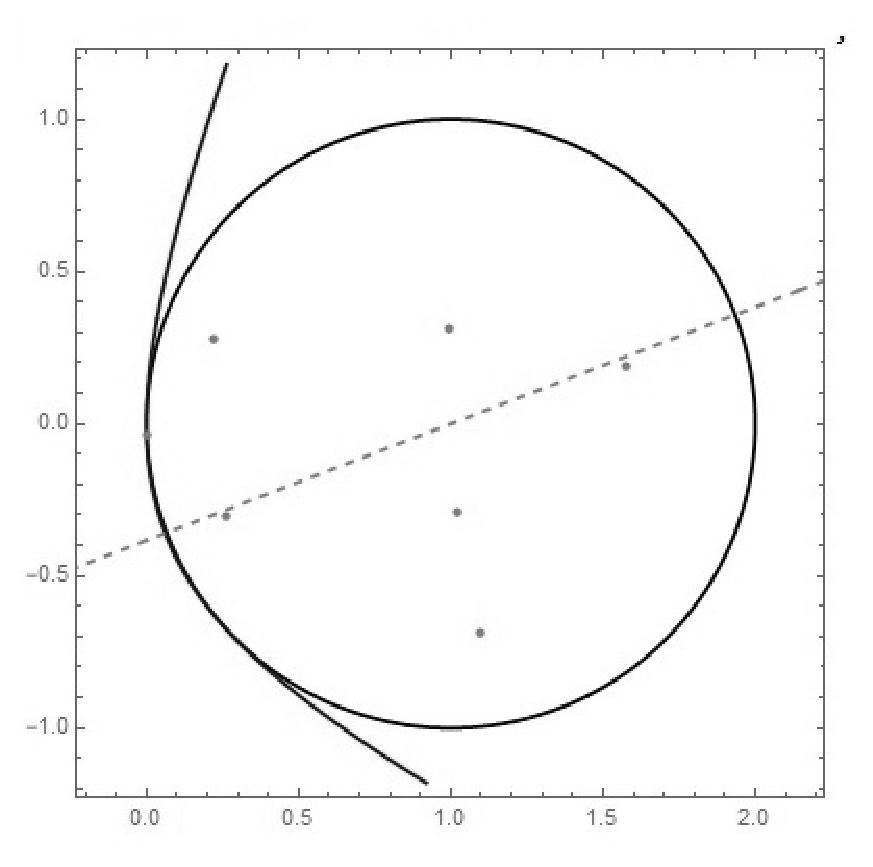
\includegraphics[width=\linewidth]{phaseB}
    \caption{Соответствует верхней стороне клина. Квадратичная форма здесь представляет собой гиперболу.}
    \label{fig:phaseB}
  \end{subfigure}
  \caption{Несколько точек фазового портрета для клина, изображенного на Рис. \ref{image10} с указанием области соответствующих квадратичных форм из \eqref{EQ_quadratic}.}
  \label{fig:phaseAB}
\end{figure}

%\begin{figure}[ht]
%  \centering
%  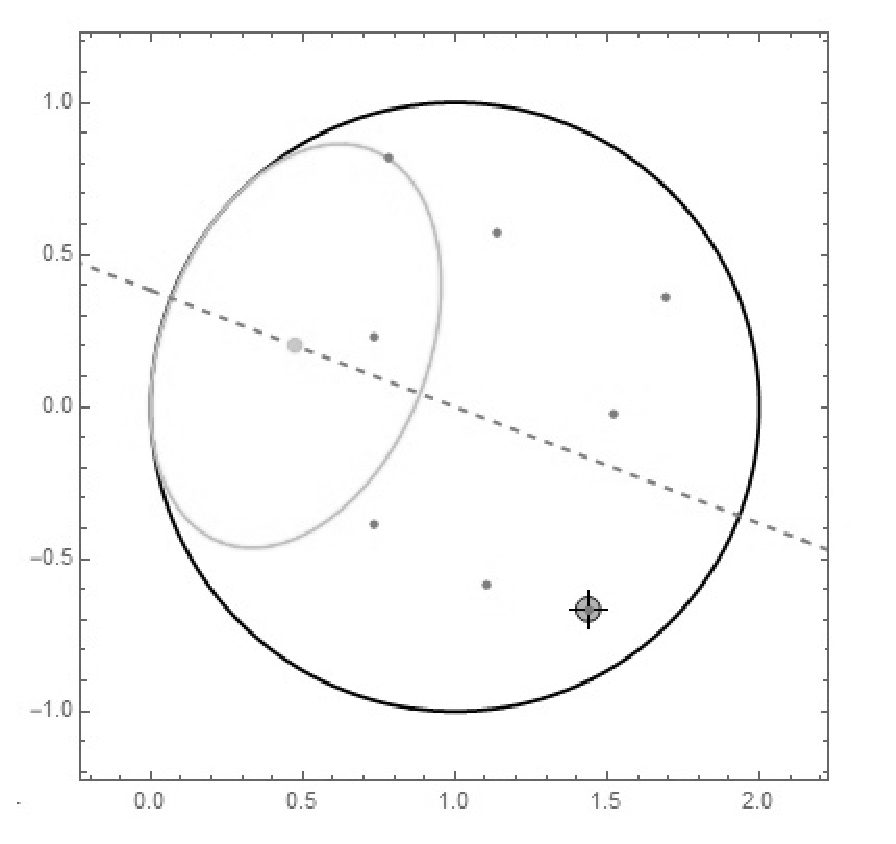
\includegraphics[width=100.5mm, height=52.2mm, viewport=3mm 4mm 205mm 292mm]{phaseA} а)\\
%%   \caption{}\label{image6}
%  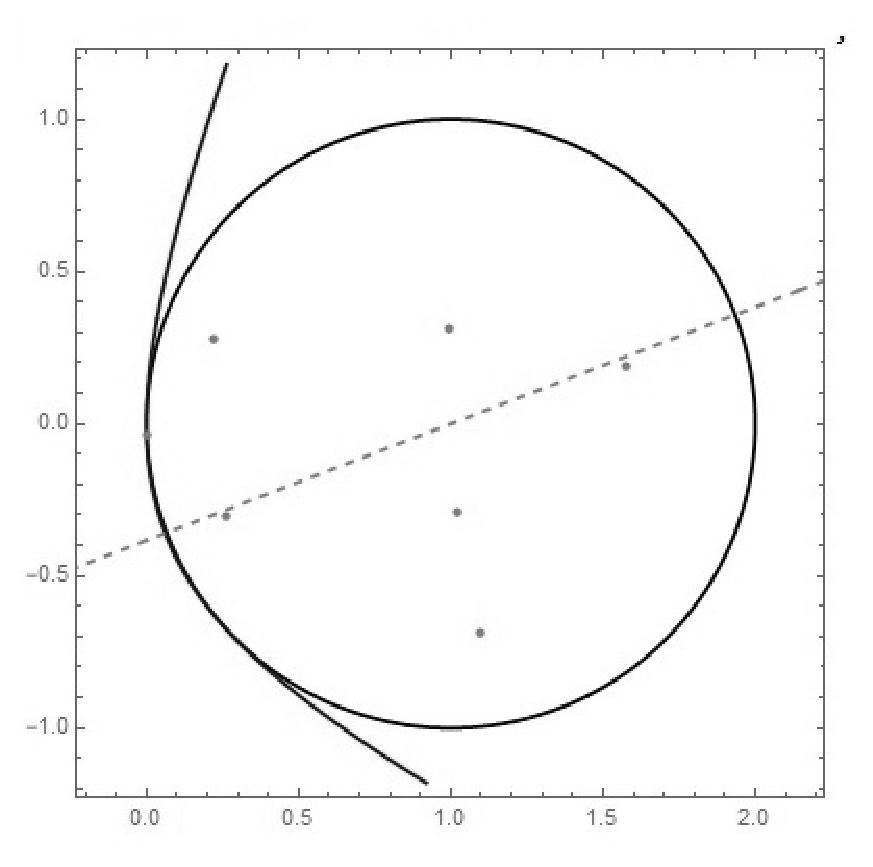
\includegraphics[width=100.5mm, height=52.2mm, viewport=3mm 4mm 205mm 292mm]{phaseB} б)\\
%  \caption{}\label{phaseAB}
%\end{figure}

Найдем  отображение для переменных $d ,\tau$. Это отображение имеет два варианта в зависимости от областей, которые буду определены далее. Если после отражения частица падает на ту же сторону, то согласно \eqref{GrindEQ__11_} отображение переходит в 
\begin{equation}
 \label{GrindEQ__21_6} \bar{\tau }=\tau -2 d \tg \alpha_{i},\:\bar{d}=d
\end{equation}

В случае падения на другую сторону будет несколько сложнее. Поскольку, после первого соударения $d_{i} $ не меняется (вспоминаем «квазиодномерность» при отражении от наклонной стенки), а становится $d_{j} $ \textit{только} в момент второго соударения, то из \eqref{GrindEQ__8_} полагая $b=0$ и учитывая \eqref{GrindEQ__11_2_4_} должны выполняться следующие соотношения:
%Пусть после столкновения с одной из стенок, частица затем сталкивается с другой. Это область фокусов помечена желтым цветом на Рис.\ref{image10} и как это следует из общего принципа показанного раннее на Рис.\ref{image6_7}(б) является пересечением областей определения для каждой из стенок. Интересно отметить, что на Рис.\ref{image10}. отсутствует красная область, поскольку область определения для 2-й (верхней) стенки лежит полностью внутри области для 1-й стенки, что определяет невозможность дважды подряд столкнуться со верхней стенкой. Поскольку, после первого соударения $d_{i} $ не меняется (вспоминаем «квазиодномерность» при отражении от наклонной стенки), а становится $d_{j} $ \textit{только} в момент второго соударения, то из \eqref{GrindEQ__8_} и учитывая \eqref{GrindEQ__11_2_4_} должны выполняться следующие соотношения:

%\begin{equation} \label{GrindEQ__21_2} \begin{array}{l} {d_{i} =4\left(1-b+\left(Y-b\right)\cos \, 2\alpha _{i} -X\sin \, 2\alpha _{i} \right)\sin ^{2} \alpha _{i} ,} \\ {d_{j} =4\left(1-b+\left(Y-b\right)\cos \, 2\alpha _{j} -X\sin \, 2\alpha _{j} \right)\sin ^{2} \alpha _{j} } \end{array} \end{equation}

\begin{equation} \label{GrindEQ__21_2} \begin{array}{l} {d_i=1-X \sin 2 \alpha _i+Y \cos 2 \alpha _i ,} \\ {d_j=1-X \sin 2 \alpha_j+Y \cos 2 \alpha _j } \end{array} \end{equation}

Где $\left(X,Y\right)$ - координаты фокуса параболы \textit{между} столкновениями, a $i\ne j$ . Применяя рассуждения подобные тем, которые мы проделали для получения \eqref{GrindEQ__10_1_}, мы можем переписать это уравнение так

%\begin{equation} \label{GrindEQ__22_} Y=1-d_{i} \nu _{i} =1-d_{j} \nu _{j}  \end{equation}

\begin{equation} 
 \label{GrindEQ__22_} 
1-Y=\frac{(\tau_{i}  \cos \alpha_{i} +d_{i} \sin \alpha_{i} )^2}{d_{i}}=\frac{(\tau_{j}  \cos \alpha_{j} -d_{j} \sin \alpha_{j} )^2}{d_{j}}
\end{equation}
%
%Поскольку, $\nu _{i} $ в данном случае соответствует траектории сразу \textit{до }и \textit{после} первого столкновения, а $\nu _{j} $ \textit{до} и \textit{после }второго, то согласно \eqref{GrindEQ__11_2_2_} и аналогично \eqref{GrindEQ__10_1_}
%
%\begin{equation} \label{GrindEQ__23_} \nu _{i} =\frac{\left(1-\tau _{i} \right)^{2} }{4} ,\; \nu _{j} =\frac{\left(1+\tau _{j} \right)^{2} }{4}  \end{equation}

Решая совместно \eqref{GrindEQ__21_2} и \eqref{GrindEQ__22_} получим

%\begin{equation} \label{GrindEQ__24_}\begin{array}{l} {d_{j} =D\left(d_{i} ,\tau _{i} ,\alpha _{i} ,\alpha _{j} ,b\right)=} \\ {4\left(1-b-\frac{\sin 2\alpha _{j} }{\sin 2\alpha _{i} } \left(1-b-\frac{d_{i} }{4\sin ^{2} \alpha _{i} } \right)-\left(1-b-d_{i} \frac{\left(1-\tau _{i} \right)^{2} }{4} \right)\frac{\sin 2\left(\alpha _{j} -\alpha _{i} \right)}{\sin 2\alpha _{i} } \right)\sin ^{2} \alpha _{j} } \end{array} \end{equation}
\begin{equation} 
 \label{GrindEQ__24_}
{d_j} =D\left(d_{i} ,\tau _{i} ,\alpha _{i} ,\alpha _{j}\right)= 1 + \frac{{\sin 2{\alpha _j}}}{{\sin 2{\alpha _i}}}\left( {{d_i} - 1} \right) + \frac{{\sin 2\left( {{\alpha _j} - {\alpha _i}} \right)}}{{\sin 2{\alpha _i}}}\left( {\frac{{{{\left( {d\sin {\alpha _i} - {\tau _i}\cos {\alpha _i}} \right)}^2}}}{{{d_i}}} - 1} \right) 
\end{equation}

%\begin{equation} \label{GrindEQ__25_} \tau _{j} =T\left(d_{i} ,\tau _{i} ,d_{j} \right)=-1\pm \left(1-\tau _{i} \right)\sqrt{\frac{d_{i} }{d_{j} } }\end{equation}
\begin{equation} 
 \label{GrindEQ__25_} {\tau _j} = T^{\pm }\left(d_{i} ,\tau _{i} ,d_{j},\alpha_i,\alpha_j \right)= - {d_j}\tan {\alpha _j} \pm \frac{{{d_i}\sin {\alpha _i} - {\tau _i}\cos {\alpha _i}}}{{\cos {\alpha _j}}}\sqrt {\frac{{{d_j}}}{{{d_i}}}}
\end{equation}


%Теперь разделим обе части на $4(1-b)$ и переопределим $d = 4(1-b) d$
%
%\begin{equation} \label{GrindEQ__25_1} {d_j} = D\left(d_{i} ,\tau _{i} ,\alpha _{i} ,\alpha _{j} \right)={\sin ^2}{\alpha _j}\left( {1 + \frac{{\sin \left( {{\alpha _i} - 2{\alpha _j}} \right)}}{{\sin {\alpha _i}}} + \frac{{{d_i}}}{{\sin 2{\alpha _i}}}\left( {\frac{{\sin 2{\alpha _j}}}{{{{\sin }^2}{\alpha _i}}} + \sin 2\left( {{\alpha _j} - {\alpha _i}} \right){{\left( {1 - \tau } \right)}^2}} \right)} \right)\end{equation}
%таким образом избавляясь от параметра $b$ в отображении \eqref{GrindEQ__24_}, а \eqref{GrindEQ__25_} не меняет своего вида.
 
При этом оказывается, что в \eqref{GrindEQ__25_} при выборе знака допустим \textit{только} «+», если мы хотим получить именно правильную траекторию частицы в рассматриваемом клине. Это можно качественно понять устремив $\beta \to \alpha $ (очень узкий клин) . При  почти точном равенстве, траектория частицы будет «биться» между двумя фокусами. И соответственно не может быть траектории, при которой бы частица дважды подряд попала на одну сторону. Т.е. положив в \eqref{GrindEQ__25_} $d_{i} =d_{j} $ корень со знаком «$-$» даст нам соотношение \eqref{GrindEQ__21_6}, чего не должно быть (соответствует попадание на ту же стенку),  и потому нужно выбирать знак «$+$». Оказывается, это остается верным для любого соотношения наклонов стенок. Интересно отметить, что $D\left(d_{i} ,\tau _{i},\alpha _{i}+\pi ,\alpha _{i} \right) = d_j=d_i$ и $=T^{+}\left(d_i,\tau_i,d_j,\alpha_i+\pi,\alpha_i\right)=\tau_j=\tau_i-2 d_i \tg \alpha_{i}$ и совпадает с отображением \eqref{GrindEQ__21_6}.

Теперь рассмотрим условия, при которых частица после \textit{первого }соударения не сталкивается с другой стенкой, а снова падает на нее же. На Рис.\ref{image10} эта зона отмечена темно серым цветом. В результате отображение должно выглядеть согласно \eqref{GrindEQ__21_6}.
%$\bar{d}_{i} =d_{i} ,\quad \bar{\tau }_{i} =\tau _{i} -2$.
Такой вариант возможен в двух случаях: либо из \eqref{GrindEQ__24_} $d_{j} \le 0$, либо для $\left(d ,\tau \right)$ не выполняется соотношение \eqref{GrindEQ__21_5}. В первом случае, чтобы найти границу области мы должны приравнять нулю левую часть уравнения \eqref{GrindEQ__24_}. В результате получим уравнение квадратичной  формы, которое запишем сразу в каноничной форме
\begin{equation} \label{EQ_quadratic}
A{\left( {\left( {d - {d_0}} \right)\cos \left( {\alpha  - \beta } \right) + \left( {\tau  - {\tau _0}} \right)\sin \left( {\alpha  - \beta } \right)} \right)^2} + B{\left( {\left( {d - {d_0}} \right)\sin \left( {\alpha  - \beta } \right) - \left( {\tau  - {\tau _0}} \right)\cos \left( {\alpha  - \beta } \right)} \right)^2} = 1
\end{equation}
где 
\begin{equation} \label{GrindEQ__26_2}
\{ A,B\}  = \frac{{\sin \beta }}{{\cos \alpha \sin \left( {\beta  - \alpha } \right)}}\{ \frac{{{\mathop{\rm tg}\nolimits} \beta }}{{tg\left( {\beta  - \alpha } \right)}},\;1\} ,\;\{ {d_0},{\tau _0}\}  = \frac{{\sin \left( {\beta  - \alpha } \right)}}{{\sin \beta }}\{ \cos \alpha ,\sin \alpha \}
\end{equation}
\begin{figure}[h]
\center{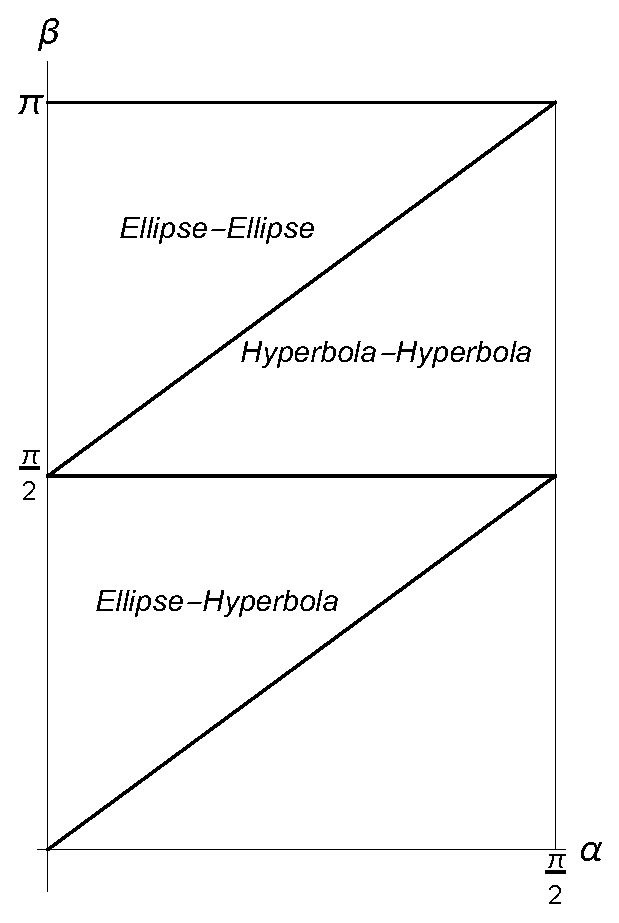
\includegraphics[width=0.25\linewidth]{quadratic}}
\caption{На диаграмме показаны в виде пар варианты квадратичной формы \eqref{EQ_quadratic} для обеих сторон в зависимости от соотношения углов. Здесь $0<\alpha<\pi/2$ и $\alpha<\beta<\pi$}
\label{fig:quadratic}
\end{figure}
откуда видно, что оси квадратичной формы повернуты на угол $\beta-\alpha$ относительно системы отсчета и ее геометрический центр находится в точке с координатами $\left(d_{0},\:\tau_{0}\right)$ (см. Рис. \ref{fig:phaseAB})
% и точка выходит за соответствующие зоны показанные на Рис.\ref{image11}. 
%Кривая, соответствующая касанию c {верхней} стенкой и изображенной синим пунктиром (Рис. \ref{image11}) можно найти из уравнения $d_{2} =0=D\left(d ,\tau ,\alpha _{1} ,\alpha _{2}\right)=D\left(d ,\tau ,\alpha ,\beta \right)$:
%
%\begin{equation} \label{EQ_quadratic}d=\frac{2 \sin 2 \alpha  \sin \alpha \cos \beta \sin (\alpha -\beta )}{(1-\tau )^2 \sin ^2\alpha  \sin 2 (\alpha -\beta )-\sin 2 \beta }\end{equation}
%т.е. если точка на Рис.\ref{image11} справа от этой кривой, то частица снова сталкивается с нижней стенкой.

Таким образом, окончательно получаем отображение:

\begin{equation} \label{GrindEQ__26_}\bar{i}=\left[\begin{array}{c} {i,\quad D\left(d_{i} ,\tau _{i} ,\alpha _{i} ,\alpha _{inc\left(i\right)} \right)<0\vee R\left(D_{i\; inc(i)} ,T^{+}_{i\; inc(i)},0\right)>0} \\ {inc\left(i\right)} \end{array}\right. \end{equation}

\begin{equation} \label{GrindEQ__27_}\bar{d}=\left[\begin{array}{c} {d,\; \bar{i}=i} \\ {D\left(d_{i} ,\tau _{i} ,\alpha _{i} ,\alpha _{\bar{i}}\right)} \end{array}\right. \end{equation}

\begin{equation} \label{GrindEQ__28_}\bar{\tau }=\left[\begin{array}{c} {\tau -2 d \tg \alpha_{i},\; \bar{i}=i} \\ {T^{+}\left(d_{i} ,\tau _{i} ,\bar{d},\alpha_i,\alpha_{\bar{i}} \right)} \end{array}\right. \end{equation}

Где $inc\left(i\right)=\left[\begin{array}{c} {1,\; \; i=2} \\ {2,\; \; i=1} \end{array}\right. $ , $D_{i\; inc(i)} =D\left(d_{i} ,\tau _{i} ,\alpha _{i} ,\alpha _{inc\left(i\right)}\right),\; T^{\pm }_{i\; inc(i)} =T^{\pm }\left(d_{i} ,\tau _{i} ,d_{i\; inc\left(i\right)},\alpha _{i} ,\alpha _{inc\left(i\right)} \right)$. Фактически, $inc\left(i\right)$ -- это циклический инкремент стороны.

%\begin{figure}[h]
%\center{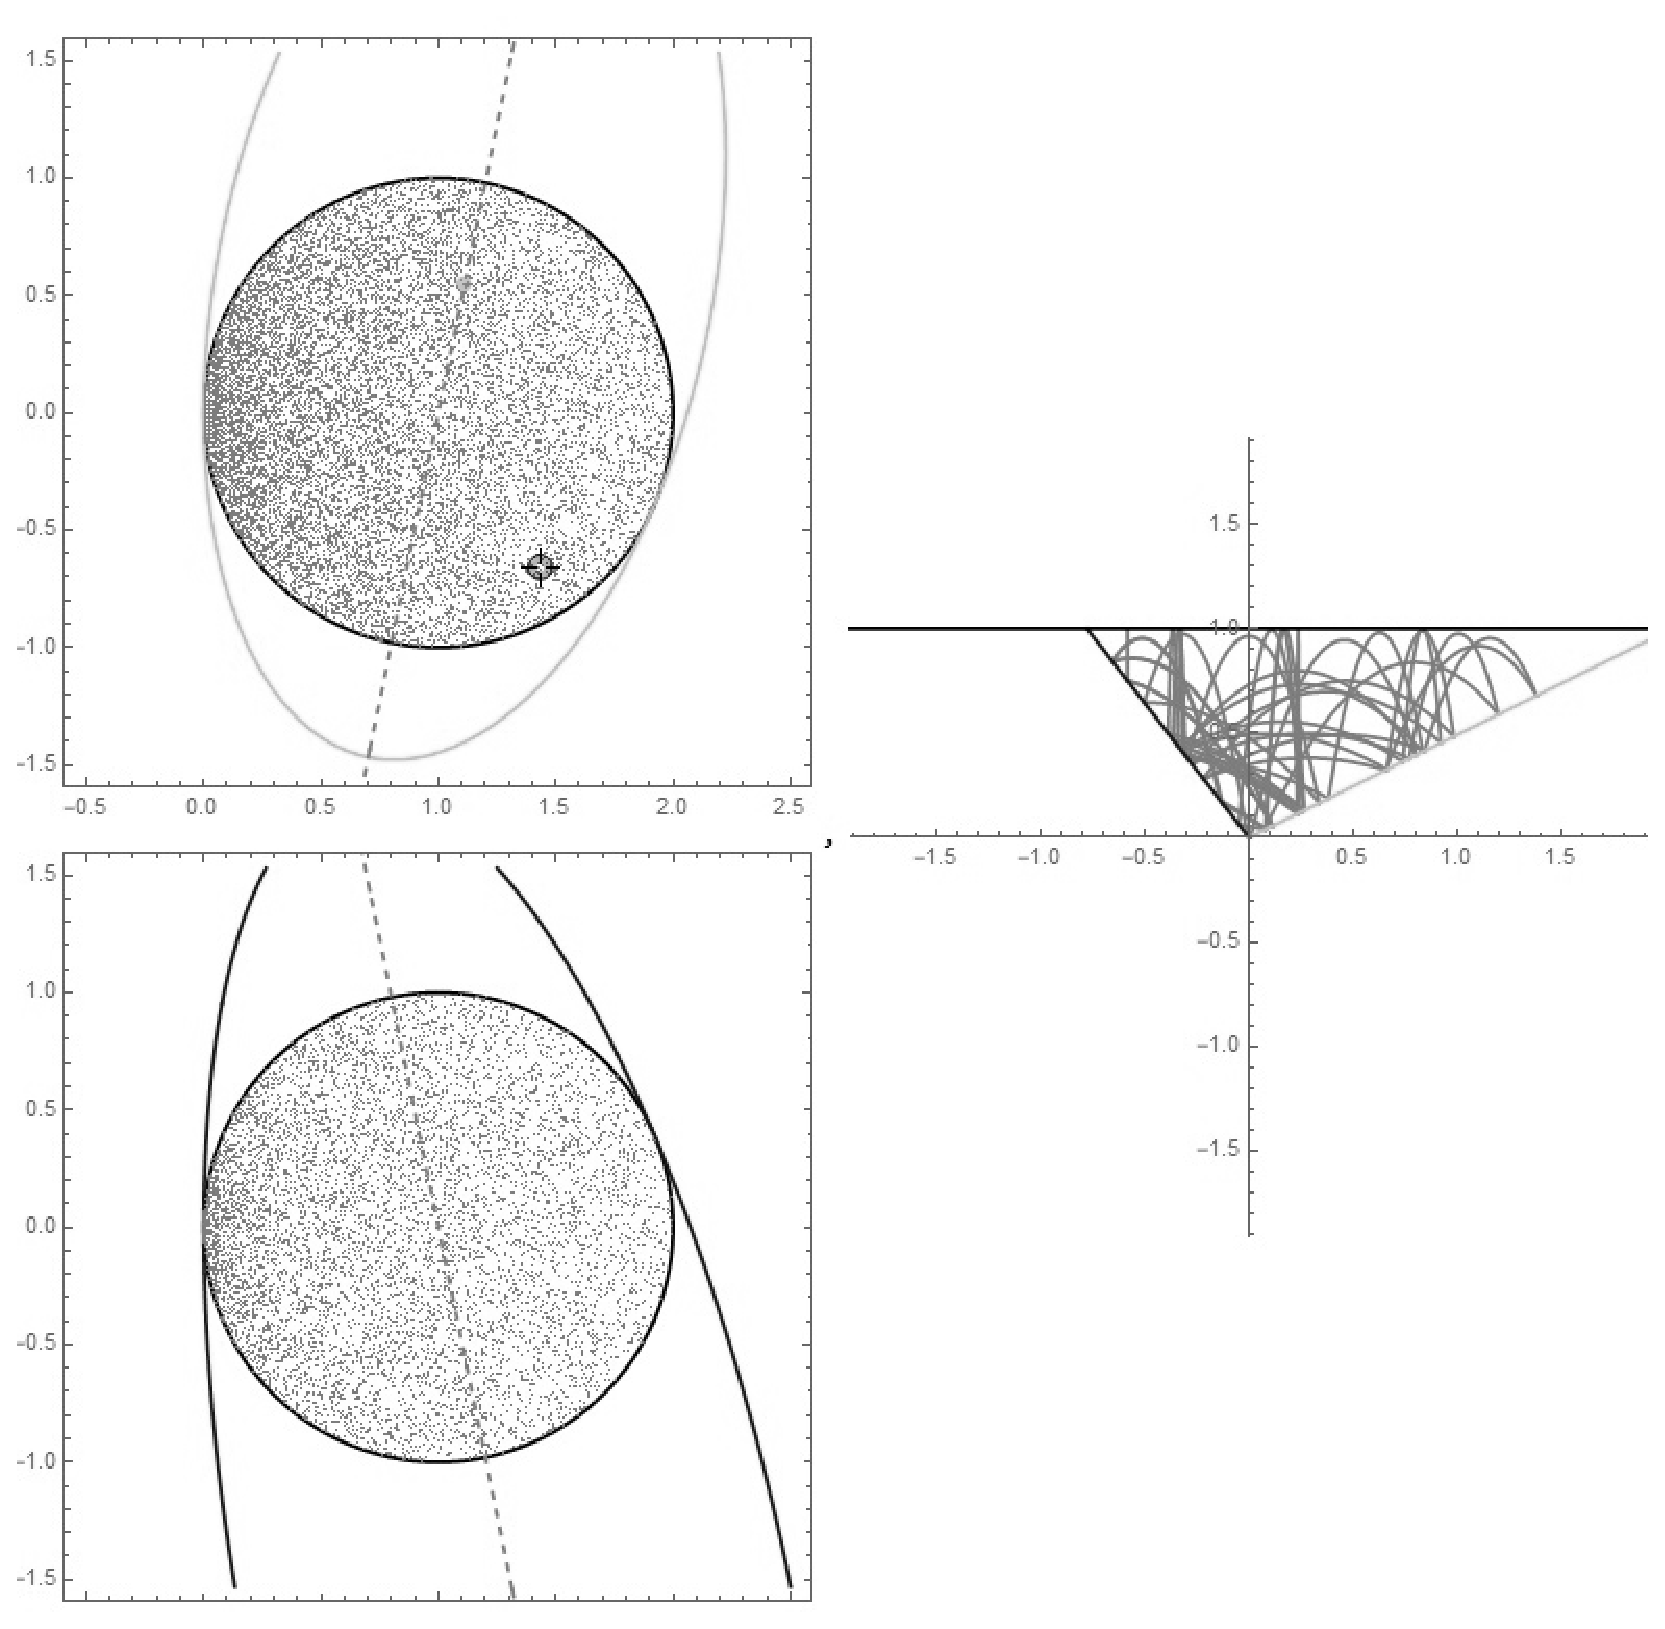
\includegraphics[width=0.8\linewidth]{obtuse}}
%\caption{Типичный фазовый портрет для тупоугольного клина. Полностью хаотичный с отсутствием остойчивых областей.}
%\label{obtuse}
%\end{figure}

\begin{figure}
    \centering
    \begin{subfigure}[b]{0.3\textwidth}
        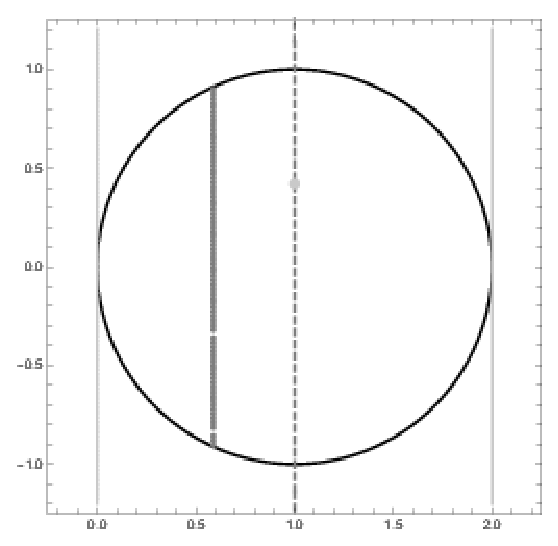
\includegraphics[width=\textwidth]{right_angle_a}
%        \caption{}
        \label{fig:right_angle_a}
    \end{subfigure}
    ~ %add desired spacing between images, e. g. ~, \quad, \qquad, \hfill etc. 
      %(or a blank line to force the subfigure onto a new line)
    \begin{subfigure}[b]{0.3\textwidth}
        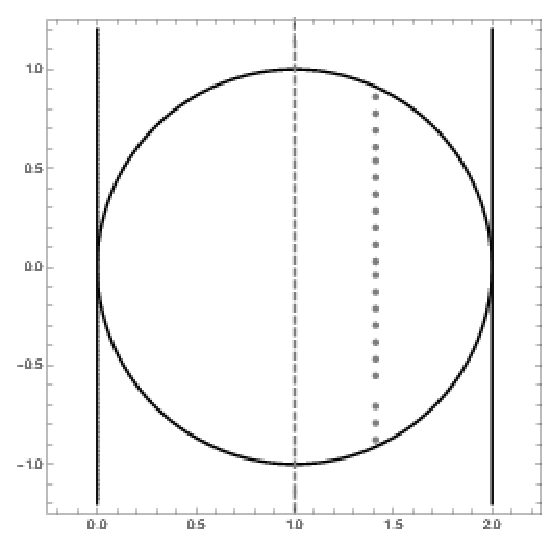
\includegraphics[width=\textwidth]{right_angle_b}
%        \caption{A tiger}
        \label{fig:right_angle_b}
    \end{subfigure}
    ~ %add desired spacing between images, e. g. ~, \quad, \qquad, \hfill etc. 
    %(or a blank line to force the subfigure onto a new line)
    \begin{subfigure}[b]{0.3\textwidth}
        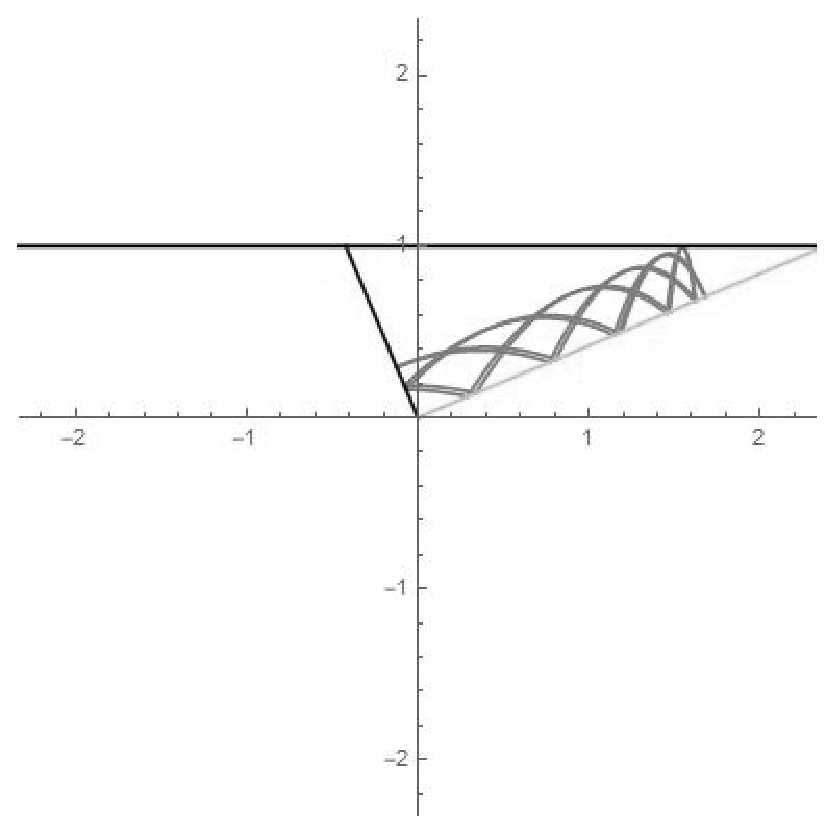
\includegraphics[width=\textwidth]{right_angle}
%        \caption{A mouse}
        \label{fig:right_angle_c}
    \end{subfigure}
    \caption{Типичные фазовые портреты для каждой из сторон прямоугольного клина и соответствующая траектория в нем. Как видно, все точки расположенные на вертикальной линии.}\label{fig:right_angle}
\end{figure}


Это отображение уже является однозначным. На Рис.\ref{fig:phaseAB} изображено несколько точек фазового портрета, соответствующие траектории частицы, изображенной на Рис.\ref{image10}. Существенную роль в качественном анализе фазового портрета играет квадратичная форма \eqref{EQ_quadratic}, а именно отношение $\dfrac{A}{B}=\dfrac{tg\beta}{tg\left(\beta-\alpha\right)}$. При $|\beta-\alpha|=\pi/2$, т.е. при прямоугольном клине независимо от наклона центральной оси клина, квадратичная форма вырождается в две прямые c уравнением $\left(d-1\right)^2=1$. При этом из \eqref{GrindEQ__24_} следует, что $d_j=2-d_i$ и такой портрет представляет собой точки, лежащие на двух вертикальных линиях (см. Рис. \ref{fig:right_angle}).

 При тупоугольном клине ($|\beta-\alpha|>\pi/2$) отсутствуют устойчивые точки и фазовый портрет является полностью хаотическим (см. Рис. \ref{obtuse}). Квадратичная форма при этом представляет собой эллипсы описанные вокруг единичного круга области определения. 
 
 При остроугольных клиньях возможны различные варианты хаоса. 
Варианты всех возможных квадратичных форм представлены на Рис. \ref{fig:quadratic}.\

В результате, мы можем обобщить диаграмму Рис.\ref{fig:angle_diagram}, вписав туда знаки отображения \eqref{GrindEQ__25_} для обеих сторон в зависимости от типа клина (см. Рис. \ref{fig:angle_diagram2}). Как видим, это отображение является универсальным для любых углов в клине с вершиной, лежащей ниже директрисы.

\begin{figure}[ht]
  \centering
  \includegraphics[width=.4\linewidth]{angle_diagram2}\\
  \caption{Типы биллиардов со знаками отображения \eqref{GrindEQ__25_} в зависимости от типа клина.}\label{fig:angle_diagram2}
\end{figure}

\begin{figure}
    \centering
    \begin{subfigure}[b]{0.3\textwidth}
        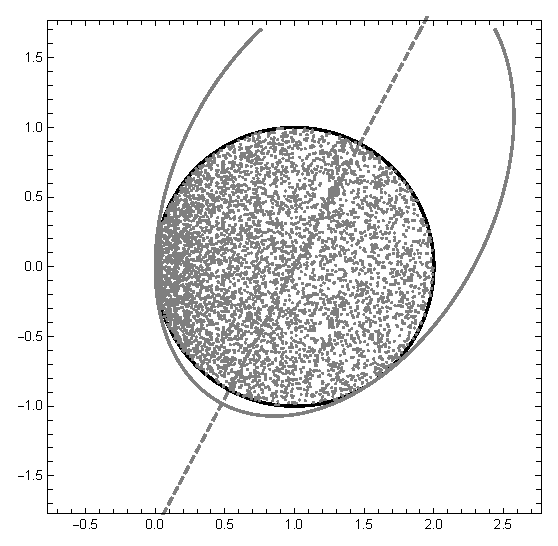
\includegraphics[width=\textwidth]{dumb_angle_a}
%        \caption{}
        \label{fig:dumb_angle_a}
    \end{subfigure}
    ~ %add desired spacing between images, e. g. ~, \quad, \qquad, \hfill etc. 
      %(or a blank line to force the subfigure onto a new line)
    \begin{subfigure}[b]{0.3\textwidth}
        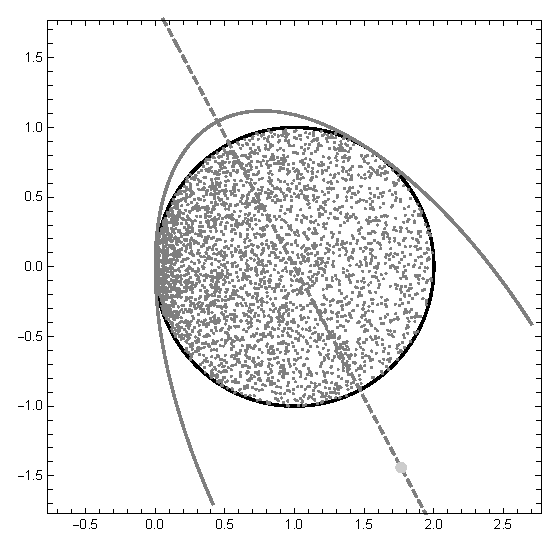
\includegraphics[width=\textwidth]{dumb_angle_b}
%        \caption{A tiger}
        \label{fig:dumb_angle_b}
    \end{subfigure}
    ~ %add desired spacing between images, e. g. ~, \quad, \qquad, \hfill etc. 
    %(or a blank line to force the subfigure onto a new line)
    \begin{subfigure}[b]{0.3\textwidth}
        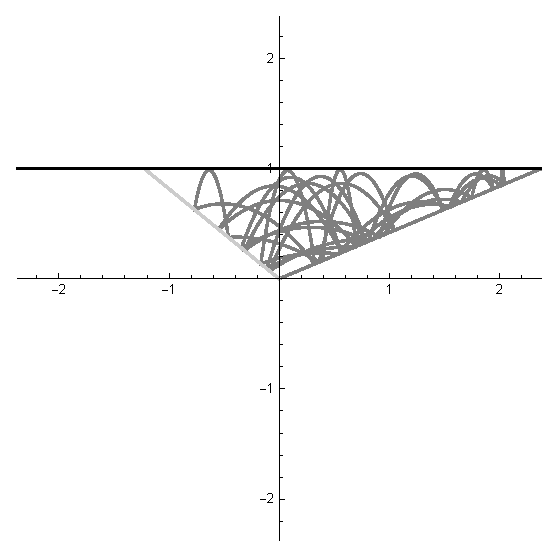
\includegraphics[width=\textwidth]{dumb_angle}
%        \caption{A mouse}
        \label{fig:dumb_angle_c}
    \end{subfigure}
    \caption{Изображены типичные фазовые портреты для каждой из сторон прямоугольного клина и соответствующая траектория в нем. Как видно, все точки расположенные на вертикальной линии.}\label{obtuse}
\end{figure}

%Как видим, точки $E_{3}$ и $E_{4}$ попадают в левую область, ограниченную \eqref{EQ_quadratic} и соответствуют попаданию дважды на одну и ту же стенку.
%Простой анализ \eqref{EQ_quadratic} показывает, что существует два существенных разделения 

%Теперь введем следующие переменные
%
%\begin{equation} \label{GrindEQ__XY} X_i=\sqrt{d_i}(\tau +1), \;\quad Y_i=\sqrt{d_i}(\tau -1) \end{equation}
%откуда
%
%\begin{equation} \label{GrindEQ__d_tau} d_i=\frac{1}{4} (X_i-Y_i)^2,\; \quad \tau =\frac{X_i+Y_i}{X_i-Y_i} \end{equation}
%подставляя теперь \eqref{GrindEQ__d_tau} в \eqref{GrindEQ__24_} и \eqref{GrindEQ__25_1} получим 
%
%  \begin{equation} \label{GrindEQ_35} X_j=\pm Y_i,\;\quad Y_j=X_j\pm \sin {{\alpha }_{j}}\sqrt{\frac{1}{\sin 2{{\alpha }_{i}}}\left( \frac{\sin 2{{\alpha }_{j}}}{\sin {{\alpha }_{i}}^{2}}{{\left( X_i-Y_i \right)}^{2}}-4\sin \left[ 2\left( {{\alpha }_{i}}-{{\alpha }_{j}} \right) \right]{{{Y_i}}^{2}}+16\cos {{\alpha }_{i}}\cos {{\alpha }_{j}}\sin \left( {{\alpha }_{i}}-{{\alpha }_{j}} \right) \right)} \end{equation}
% Если теперь положить ${\alpha }_{j} = {\alpha }_{i} = \alpha$ то \eqref{GrindEQ_35} сведется к 
% \begin{equation} \label{GrindEQ_36} X_j=\pm Y_i,\;\quad Y_j=\pm \left( 2Y_i-X_i \right) \end{equation}
% \begin{equation} \label{GrindEQ_37} X_j=\pm Y_i,\;\quad Y_j=\pm X_i \end{equation}

\section{Ориентация клиновидного биллиарда}

Рассмотрим движение массивной материальной точки в плоском клиновидном биллиарде под действием постоянного гравитационного поля (либо заряженной массивной частицы под действием постоянного электрического поля). Основное внимание сосредоточим на случае общего положения -- несимметричного клина. Ось симметрии такого клина (биссектриса) расположена произвольным образом относительно направления поля, а не параллельно, как в симметричном случае. Пусть стенки клина зафиксированы относительно направления поля. Обозначим угол отклонения оси клина от направления поля как $\phi $, а угол отклонения стенки от оси клина через $\theta $ (см. Рис.\ref{fig:in1}). Величина углов варьируются в диапазонах ${\rm 0}\le \theta \le \pi $ и ${\rm 0}<\phi \le \pi$.
%\begin{figure}[ht]
%  \centering
%  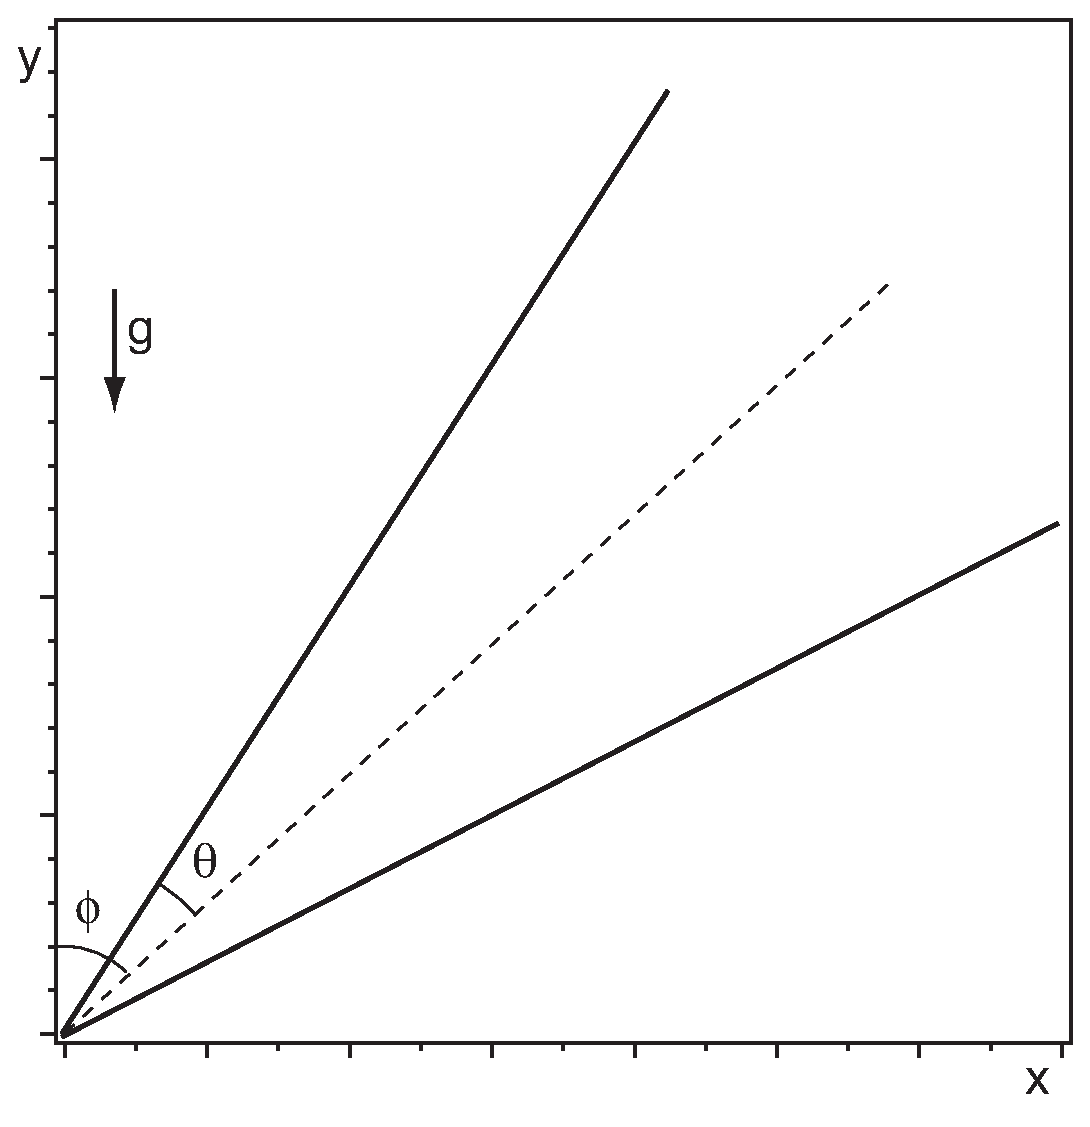
\includegraphics[width=6 cm]{in1.eps}\\
%  \caption{Показана ориентация клиновидного биллиарда по отношению к направлению поля.}\label{image1}
%\end{figure}

\begin{figure}[h!]
  \centering
  \begin{subfigure}[b]{0.3\linewidth}
    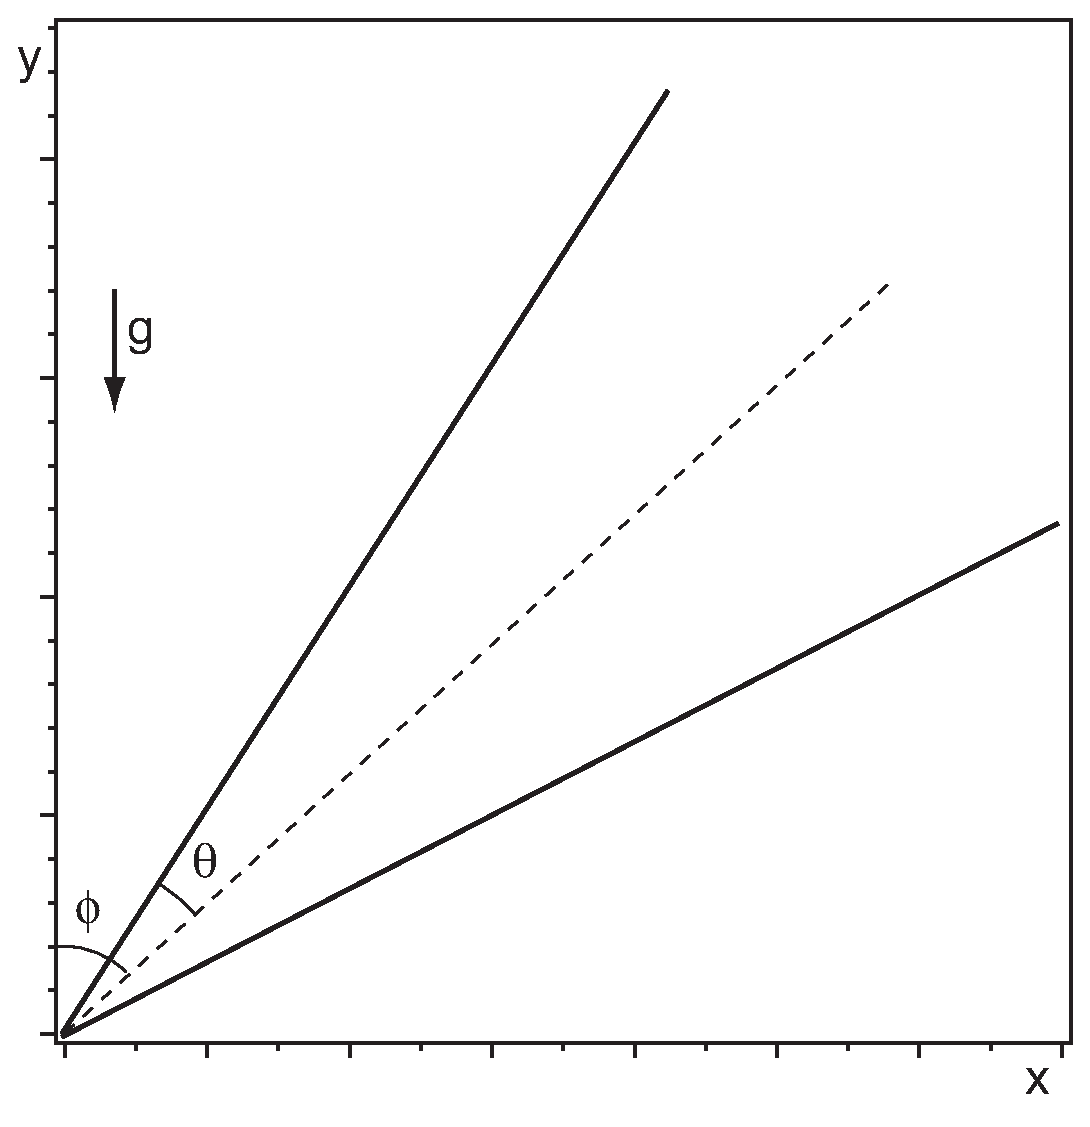
\includegraphics[width=\linewidth]{in1}
    \caption{Показана ориентация клиновидного биллиарда по отношению к направлению поля.}
    \label{fig:in1}
  \end{subfigure}
  \quad\quad\quad\quad
  \begin{subfigure}[b]{0.35\linewidth}
    \includegraphics[width=\linewidth]{angle_diagram}
    \caption{Серым показаны области углов $\phi$ и $\theta$  с разным типом движения в формате (u|d)-(u|d)/(fin|inf), где u|d - верхняя/нижняя стороны, а fin|inf - финитный/инфинитный характер движения.}
    \label{fig:angle_diagram}
  \end{subfigure}
  \caption{ }
  \label{fig:wedge}
\end{figure}

От указанных углов зависит характер движения. Траектория частицы может быть финитной или инфинитной. При $\theta+\phi<\pi /{\rm 2}$ движение частицы ограничено конечной областью в клине ограниченном сверху общей директрисой всех параболических сегментов траектории. В случае $\theta +\phi \ge \pi /{\rm 2}$ частица уходит на бесконечность, поскольку одна (или обе) из сторон клина имеют отрицательный наклон и движение частицы не имеет ограничения снизу. Кроме того, от углов также зависит какая из стенок клина является \textit{верхней}/\textit{нижней}. С \textit{верхней} стенкой частица не может столкнуться дважды подряд.  Соответственно, возможны три случая: обе стенки \textit{нижние}, обе \textit{верхние} или одна \textit{нижняя}, а вторая \textit{верхняя}. Теперь можно составить диаграмму областей углов в зависимости от этих характеристик (см. \ref{fig:angle_diagram}). В белую область попадает диапазон углов, где не существует траекторий, попадающих на разные стороны клина. Такие биллиарды являются тривиальными и мы их далее не рассматриваем.

%, где колонки - это финитное/инфинитное движение, а строки - соотношение \textit{верхних}  и \textit{нижних} стенок.

%\begin{tabular}{|p{1.3in}|p{1.4in}|p{2.in}|} \hline 
% & финитное & инфинитное \\ \hline
%н/н & $\phi + \theta \le \pi /{\rm 2}\wedge \phi < \theta $ & $\pi /{\rm 2}\le \phi +\theta \le \pi\wedge  \phi<\theta$ \\ \hline
%н/в & $\phi + \theta \le \pi /{\rm 2} \wedge \phi >\theta $ & $\pi /{\rm 2}\le \phi +\theta \le \pi \wedge  \phi >\theta$ \\ \hline 
%в/в & --- & $\pi \le \phi +\theta \le 3\pi/{\rm 2} \wedge  \phi >\theta $ \\ \hline
%\end{tabular}

Следует отметить, что среди семейства н/н инфинитных биллиардов также присутствуют и невыпуклые клинья (т.е. когда $\theta>\pi/{\rm 2}$).

% \begin{figure}[ht]
% \centering
% 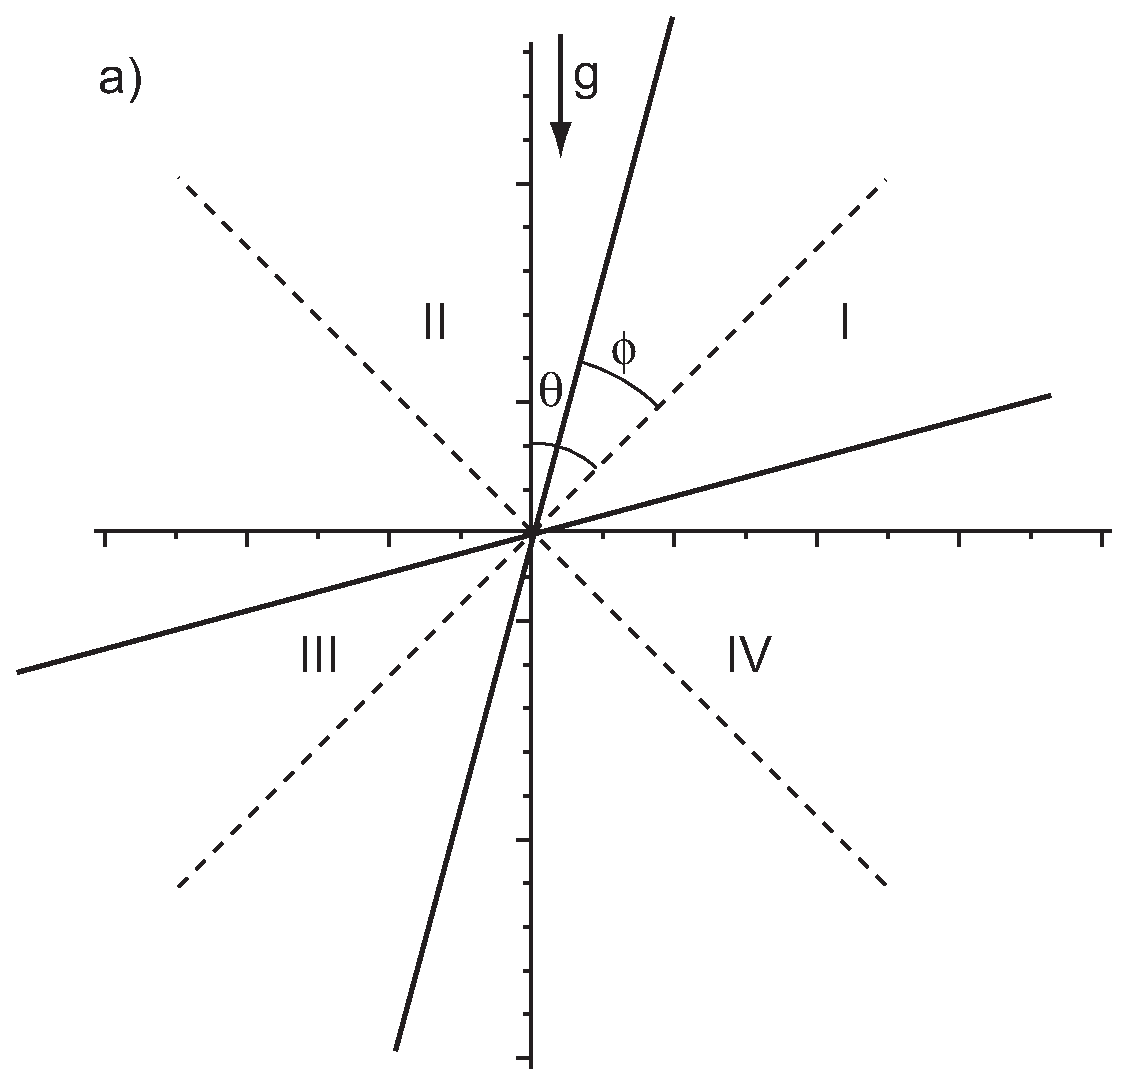
\includegraphics[width=6 cm]{in2.eps}
% 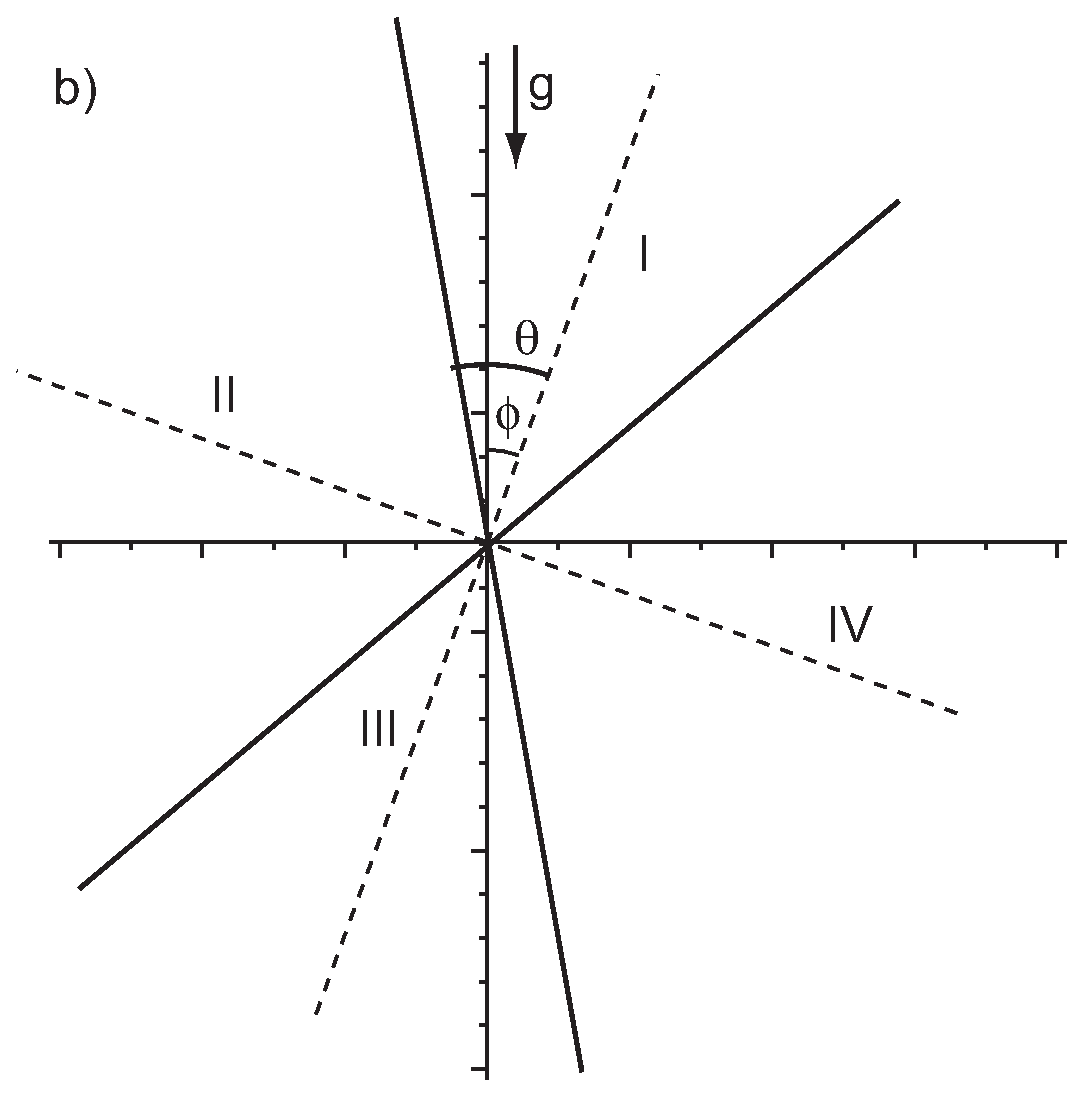
\includegraphics[width=6 cm]{in3.eps} \\
% \caption{Другой способ классификации клиновидных биллиардов.}
% \label{image2_3}
% \end{figure}

% Еще один способ классификации клиновидных биллиардов может быть по направляющим стенок. Т.е. любые две прямые делят плоскость на четыре секции, каждая из которых соответствует такому биллиарду. Тогда каждому <<финитному>> билллиарду  соответствует три <<инфинитных>>: два смежных и один вертикальный. Исключая случай, когда одна из стенок перпендикулярна направлению поля. Тогда все бильярды будут инфинитными. Под смежными клиньями мы будем понимать клинья, образующие углы  которых являются \textit{смежными.} Соответственно, образующие \textit{вертикальных} клиньев являются \textit{вертикальными} углами (см. Рис.\ref{image2_3}). С этой точки зрения мы можем рассматривать семейство из четырех выпуклых и четырех невыпуклых клиньев. Под {выпуклостью} понимается величина  углов между образующими клина. При этом, нетривиальным движением в невыпуклом клине будет только в одном случае (см. п. V ниже) и всегда является инфинитным. В свою очередь, выпуклые семейства можно разделить на два вида по финитным биллиардам - либо с двумя <<нижними>> сторонами (Рис.\ref{image2_3}(б)), либо с одной \textit{нижней} и одной \textit{верхней} (Рис.\ref{image2_3}(а)). Назовем их, соответственно, \textit{открытый} и \textit{закрытый}. Здесь римскими цифрами обозначены следующие клинья:
% \begin{description}
%   \item[I] финитный клин
%   \item[II] левый смежный инфинитный клин
%   \item[II] вертикальный инфинитный клин
%   \item[IV] правый смежный инфинитный клин
%   \item[V] невыпуклый инфинитный клин соответствует верхней области клина IV на Рис.\ref{image2_3}(а) и клина III на Рис.\ref{image2_3}(б)
% \end{description}
 Начнем с биллиарда \textit{u-d/fin} типа.

\section{Соответствие с биллиардом без поля в коружности}
 Как можно заметить отображения \eqref{GrindEQ__21_6} совпадает с отображением обычного биллиарда без поля в окружности или в круглой плоской спирали с упругой радиальной стенкой (см. Рис.~\ref{ciercle_billiard2_image}). 
\begin{figure}[ht]
  \centering
  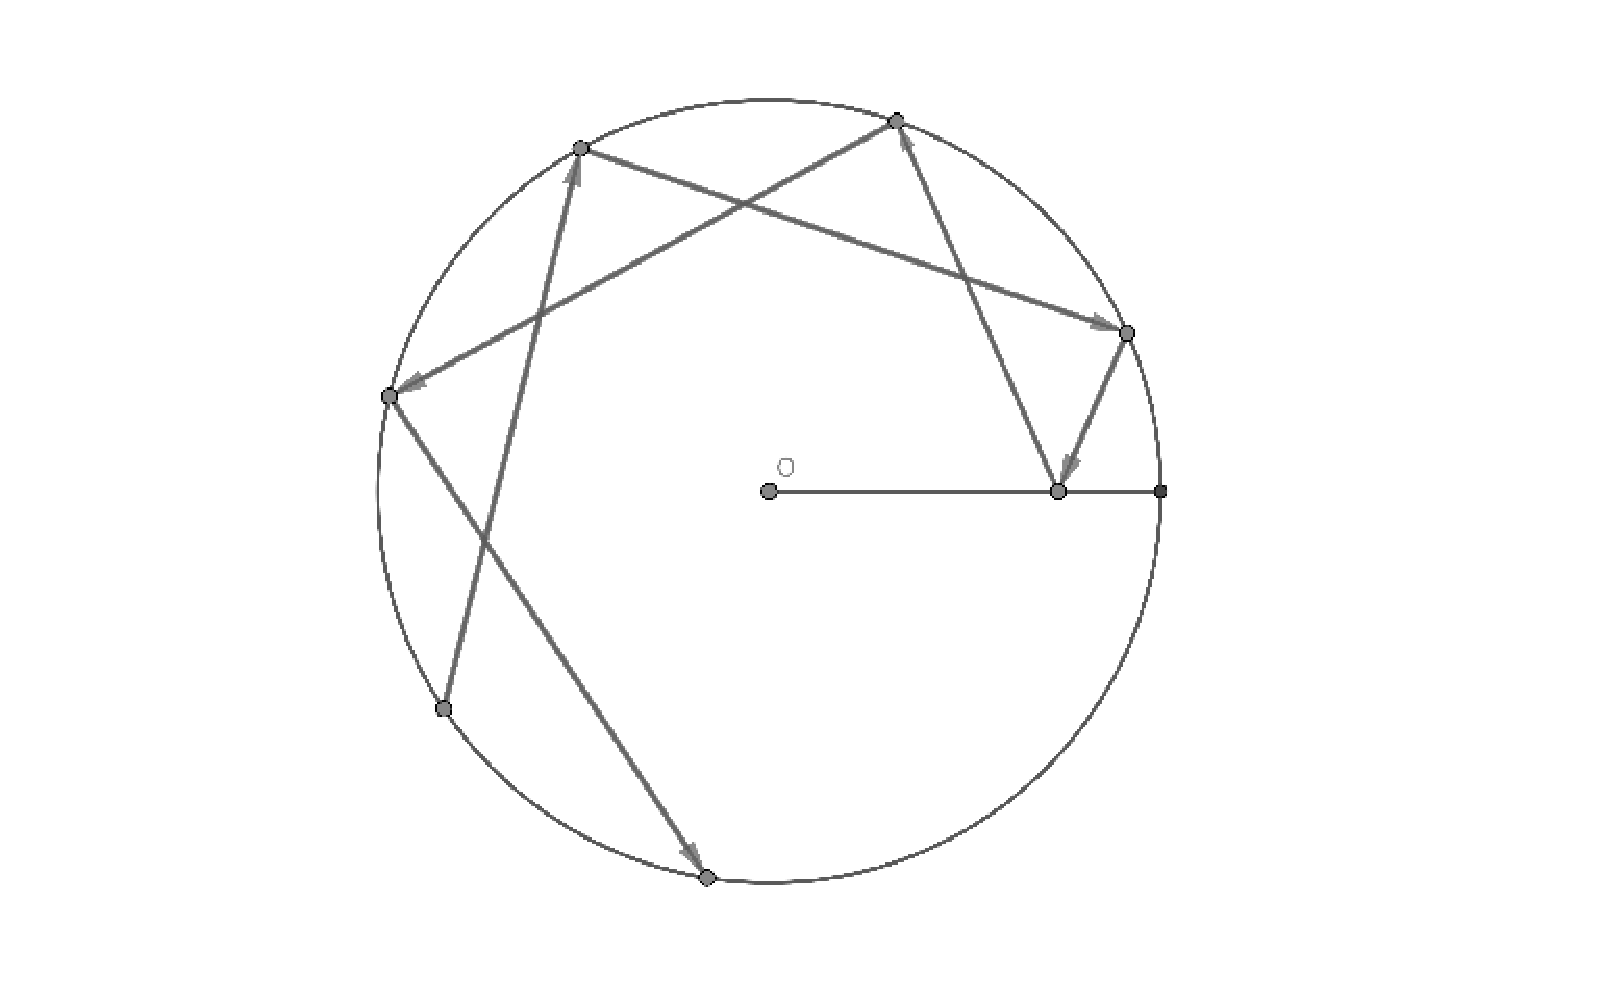
\includegraphics[width=.5\linewidth]{ciercle_billiard2_image2}\\
  \caption{Биллиард в полуограниченной по радиусу плоской спирали}\label{ciercle_billiard2_image}
\end{figure}

 Попробуем найти  параметры окружности биллиарда без поля для сопоставления с биллиардом в поле на наклонной стенке. Для удобства воспользуемся методом Шварца спрямления траектории (см. Рис.~\ref{circle5_image}).
 \begin{figure}[ht]
  \centering
  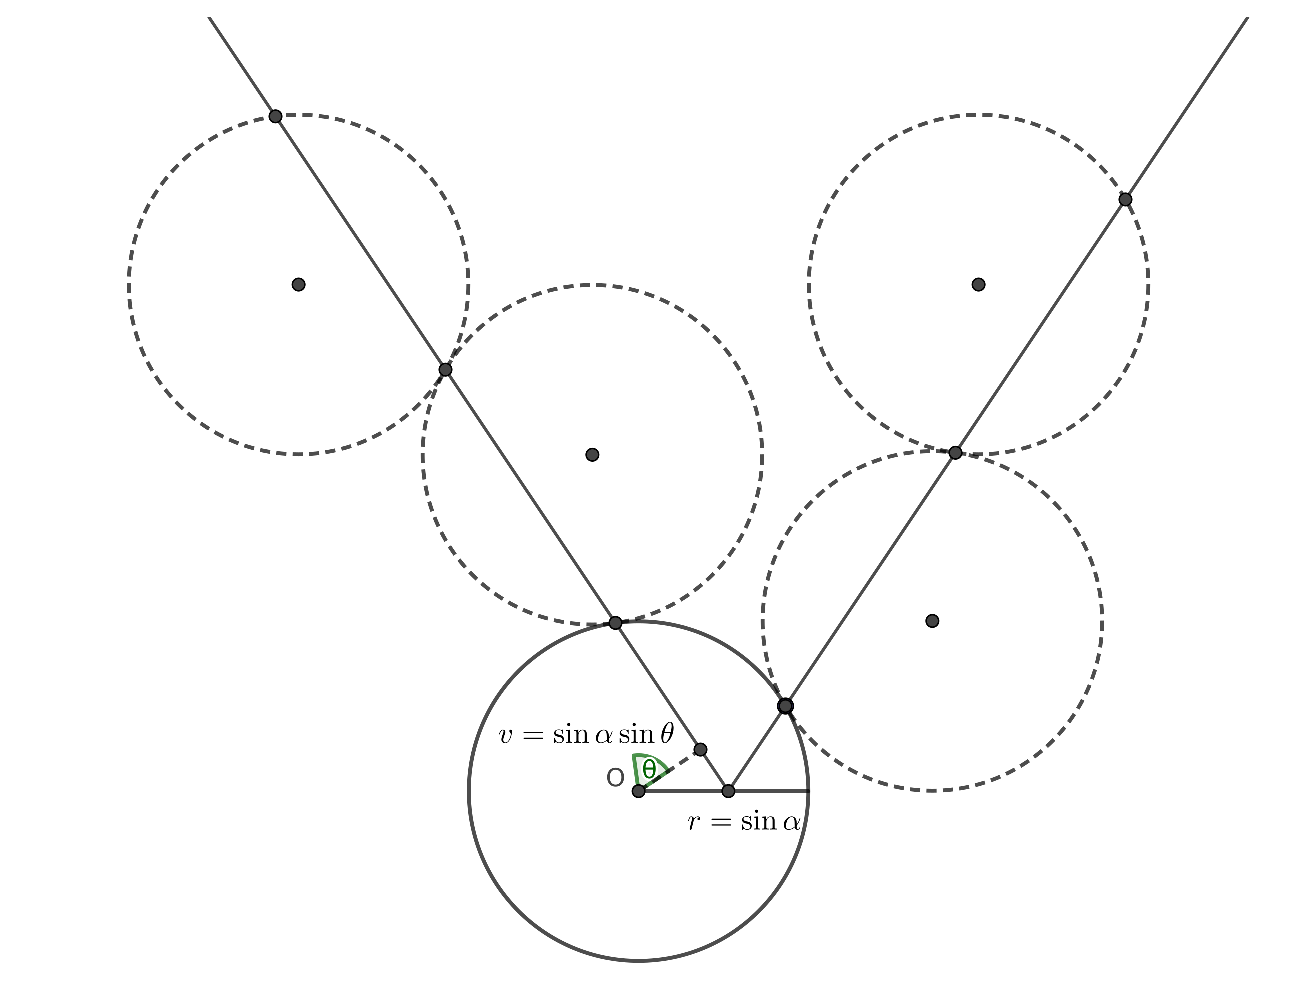
\includegraphics[width=.5\linewidth]{circle5_image.eps}\\
%   \includegraphics[width=1\linewidth]{circles1_image.eps}\\
  \caption{Спрямленный биллиард в полуограниченной спирали }\label{circle5_image}
\end{figure}
 Возьмем в качестве радиуса $\sin \alpha$ (этот выбор параметра  станет понятен позднее), где $\alpha$ тот самый угол наклона. Теперь мы легко можем построить отображение. В качестве одного из параметров возьмем половину длины хорды окружности, образованную двумя последовательными соударениями со стенкой окружности. Ясно, что при упругом отражении этот параметр (обозначим его через $v$) останется константой, а вторым параметром пусть будет условно безразмерное время $t$ с интервалом между соседними соударениями с окружностью равным 2 (без ограничения общности это всегда можно сделать). Тогда в этих переменных отображение в окружности будет выглядеть тривиально:
\begin{equation} \label{GrindEQ_38} \bar{v}=v,\;\quad \bar{t}=t+2 \end{equation}
Очевидно, что это фактически  то же самое отображение из \eqref{GrindEQ__11_2_3_} и  \eqref{GrindEQ__11_2_4_} только обращенное по времени, что непринципиально. Откуда мы можем легко найти аналогию c биллиардным отображением от наклонной плоскости в поле 
\begin{equation} \label{GrindEQ_39} v = \sqrt{d},\;\quad t=-\tau \end{equation}
Рассмотрим \eqref{GrindEQ_38} более детально. Обозначим через $\theta$ половину угла раствора хорды, тогда если $r=\sin\alpha$, то $v=\sin\theta\sin\alpha=\sqrt{d} = \sqrt{4 \tilde{X}\sin^2\alpha}$ (см. Рис.~\ref{circle5_image}). 
Откуда $\sin\theta=2\sqrt{\tilde{X}}$. Запомним этот результат. Из общих соображений можно предположить, что если биллиард на наклонной плоскости в поле сводится к биллиарду в круглой спирали без поля, то биллиард в клине в поле мог бы так же свестись к биллиарду в пересечении двух спиралей без поля. Поэтому рассмотрим теперь биллиард в пересечении двух спиралей без поля и попробуем сопоставить его параметры с биллиардом в поле. В дальнейшем будем обозначать исходный тип биллиарда в поле через $F$ (field), а сопоставляемый без поля через $C$ (circle).
Если мы возьмем два круглых биллиарда и исключим элементарные преобразования на масштаб, повороты и сдвиги, то очевидно что мы будем иметь всего два существенных параметра. Это отношение радиусов и расстояние между центрами окружностей биллиардов (см. Рис. ~\ref{two-circle4}).
% ~\ref{circles1_image}). 

% \begin{figure}[ht]
%   \centering
%   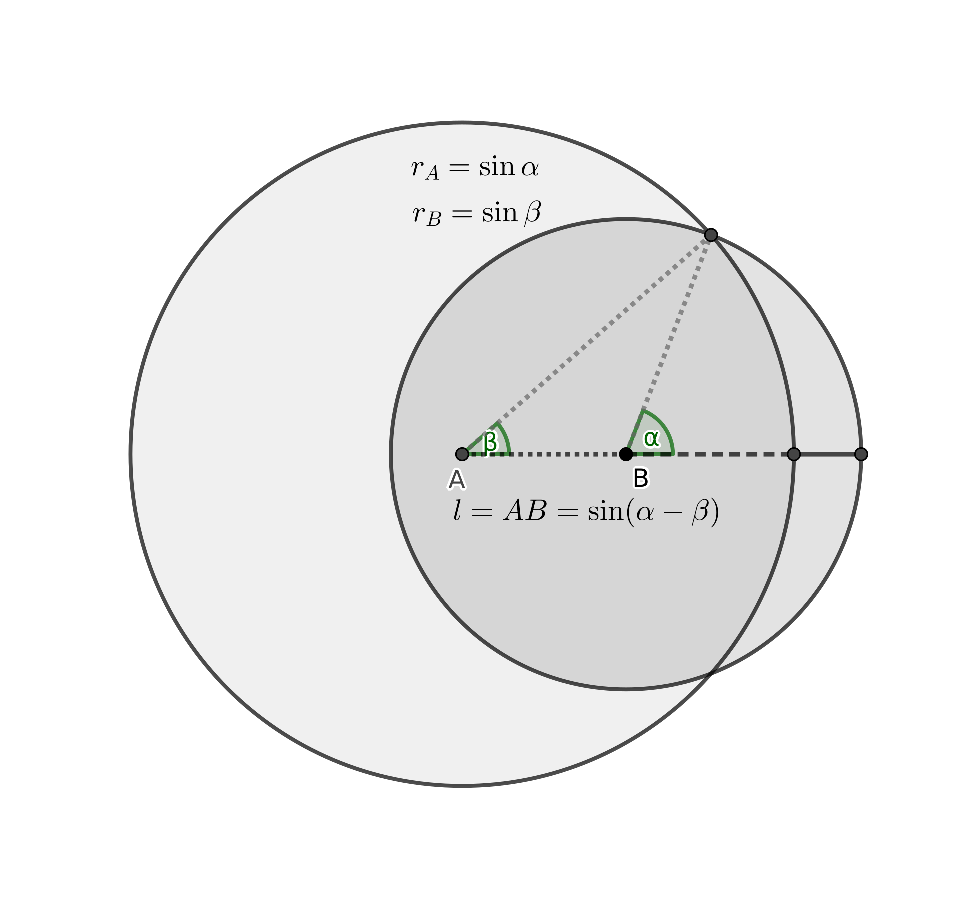
\includegraphics[width=0.9\linewidth]{circles1_image2.eps}\\
%   \caption{Пересечение биллиардов типа $C$}\label{circles1_image}
% \end{figure}

\begin{figure}[h]
\begin{minipage}[h]{0.49\linewidth}
\center{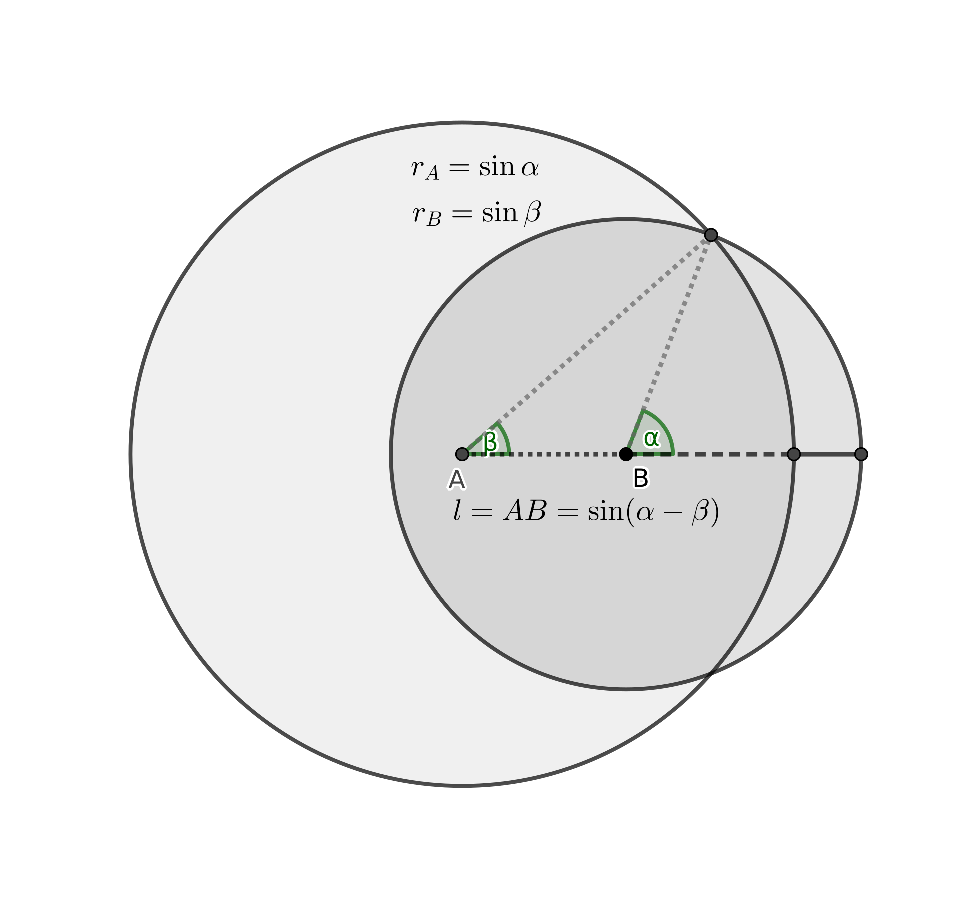
\includegraphics[width=.8\linewidth]{circles1_image2} \\ а)}
\end{minipage}
\hfill
\begin{minipage}[h]{0.49\linewidth}
\center{\includegraphics[width=.8\linewidth]{two-circle4} \\ б)}
\end{minipage}
\caption{Пересечение биллиардов типа $C$}.  
\label{two-circle4}
\end{figure}

%\begin{figure}[ht]
%  \centering
%  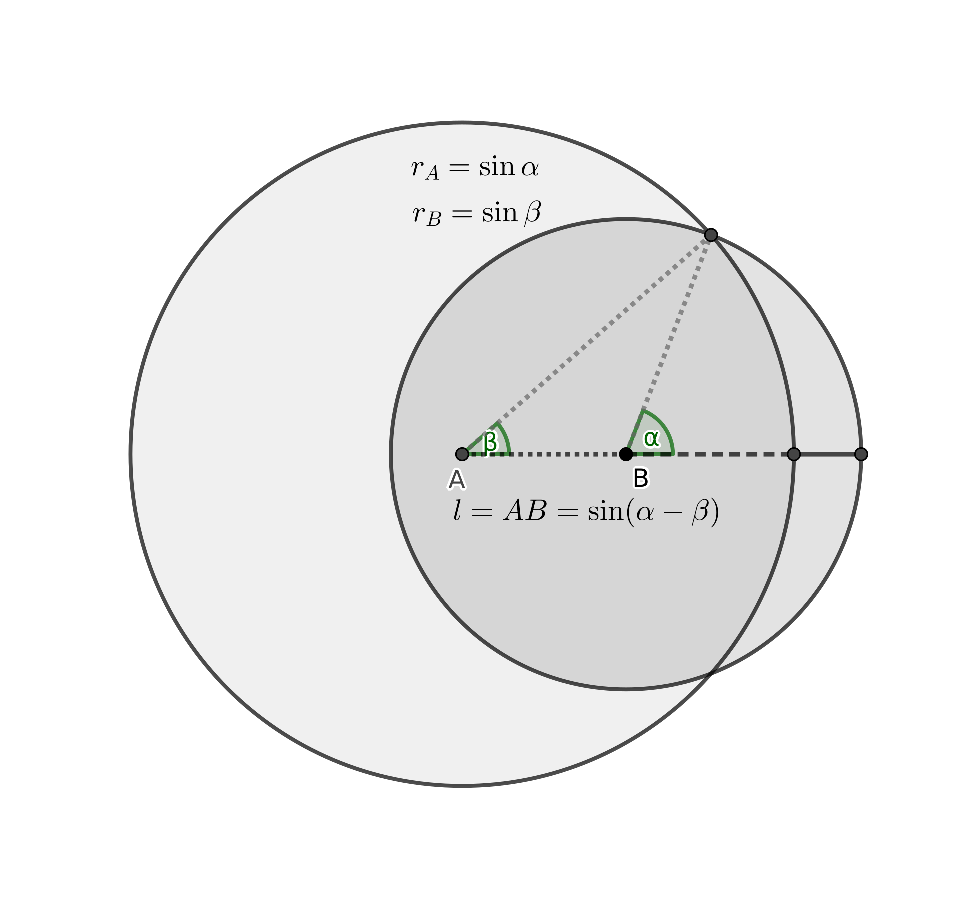
\includegraphics[width=0.55\linewidth]{circles1_image2.eps} а)\\
%%   \caption{}\label{circles1_image2}
%  \includegraphics[width=0.55\linewidth]{two-circle4.eps} б)\\
%  \caption{Пересечение биллиардов типа $C$}\label{two-circle4}
%\end{figure}
Если в качестве параметров взять углы как показано на Рис.~\ref{two-circle4}a, то тогда без ограничения общности можно найти $r_A=\sin\alpha$, $r_B=\sin\beta$, $l=\sin(\alpha-\beta)$. Либо, что асимптотически более близко (т.е. при $\alpha=\pi/2$ радиус кривизны должен становиться бесконечным, чтобы была только одна точка пересечения с окружностью, которая выродилась в прямую), $r_A=\frac{1}{\cos\alpha}$, $r_B=\frac{1}{\cos\beta}$, $l=\tg\alpha-\tg\beta$. Если мы начнем качественно рассматривать такой биллиард пересечения двух биллиардов типа $C$, то кажется, что должна быть связь с отображением для биллиарда в угле типа $F$. Например, как показано на Рис.~\ref{two-circle4}б. И действительно, при $\alpha=0$, $r_A=1$ перегородка должна выродиться в абсолютно упругую окружность в центре бесконечно малого радиуса, и при радиальном отражении (угол отражения равен нулю) траектория будет приходить в одну и ту же точку. Это легко сопоставляется с биллиардом типа $F$ с таким же углом - траектория свободно может перемещается на одинаковые расстояния и если угол падения равен нулю, то фокус такой вырожденной траектории остается на том же месте на директрисе. 
\begin{figure}[ht]
  \centering
  \includegraphics[width=.7\linewidth]{static_circles_point3.eps}\\
  \caption{стационарная точка в случае $C$}\label{static_circles_point3}
\end{figure}
При рассмотрении пересечения биллиардов типа $C$ в самом простом случае мы считаем, что радиальные перегородки обеих окружностей лежат на оси, соединяющей их центры. И хотя качественно все вроде бы хорошо с траекториями и казалось бы, что должна быть эквивалентность отображений в этом случае, это все же не так. Чтобы это показать достаточно увидеть несовпадение хотя бы качественно фазовых портретов в каком-нибудь частном случае. И такой случай можно найти. 

При $\tau=0$, $\beta=\pi-\alpha$ из \eqref{GrindEQ__25_} и \eqref{GrindEQ__24_} следует, что при отображении $d_i=d_j$. Это стационарная точка, которая есть при любых значениях параметра наклона $\alpha$ в биллиарде типа $F$. Аналогичное отображение есть и в пересечении биллиардов типа $C$ на Рис. \ref{static_circles_point3}. Но эта точка есть только для параметра $\alpha=\pi-\beta>\pi/4$ (Рис. ~\ref{two-circle4}б). Поэтому можно утверждать, что в случае радиальных перегородок лежащих на одной оси, отображения типа $C$ и $F$ не эквивалентны. Для других случаев вопрос остается открытым и может быть решен, если будет найдено отображение для случая $C$ в общем виде как для типа $F$. Пока аналитически этого сделать не удалось. 


% Возвращаясь к выбору знака в \eqref{GrindEQ__25_}, следует отметить, что знак «+» также будет и для клина $0<\alpha <{\raise0.7ex\hbox{$ \pi  $}\!\matho\left/ {\vphantom {\pi  2}} \right. \kern-\nulldelimiterspace}\!\lower0.7ex\hbox{$ 2 $}} <\beta <\pi $. Вообще, можно составить общее правило для любого из возможных клиньев, в том числе и развернутых. В выражение \eqref{GrindEQ__24_} для $d_{j} $ входит как множитель $\sin ^{2} \alpha _{j} $, и если его вынести из-под корня в \eqref{GrindEQ__25_}, то фактически знак для каждого вида клиньев условно будет зависеть от $\alpha _{j} $. Т.е. «+», при $0<\alpha _{j} <\pi $ и «--» при $-\pi <\alpha _{j} <0$. Тогда \eqref{GrindEQ__25_} можно переписать так


% \begin{equation} \label{GrindEQ__29_} \tau _{j} =-1+\frac{1-\tau _{i} }{\sin \alpha _{j} } \sqrt{\frac{d_{i} }{{1 + \frac{{\sin \left( {{\alpha _i} - 2{\alpha _j}} \right)}}{{\sin {\alpha _i}}} + \frac{{{d_i}}}{{\sin 2{\alpha _i}}}\left( {\frac{{\sin 2{\alpha _j}}}{{{{\sin }^2}{\alpha _i}}} + \sin 2\left( {{\alpha _j} - {\alpha _i}} \right){{\left( {1 - \tau } \right)}^2}} \right)} } }  \end{equation}

% Где для $\tau _{j} $ уже не будет выбора знака. Сразу отметим, что замена $\alpha _{j} \to \alpha _{j} -\pi $ подкоренное выражение не меняет, а меняет только знак перед корнем, т.е. меняет $\tau _{j}^{+} \to \tau _{j}^{-} $.

% Поэтому выбирая разные значения углов в диапазоне $\left[-\pi ,\pi \right]$, мы будем иметь разные типы клиньев (см. Рис.\ref{image2_3}). Оказывается, мы не только можем описать все виды клиньев, перечисленные в таблице во введении, но и дополнить таковыми с невыпуклым углом раствора, т.е. $\pi >\phi >{\raise0.7ex\hbox{$ \pi  $}\!\mathord{\left/ {\vphantom {\pi  2}} \right. \kern-\nulldelimiterspace}\!\lower0.7ex\hbox{$ 2 $}} $. Например, $-\pi <\alpha _{1,2} <0$ в \eqref{GrindEQ__29_} соответствует «боковым» клиньям II и IV на Рис.\ref{image2_3}(а,б) и внешней части клина IV на \ref{image2_3}(б). И далее разные соотношения знаков углов будут соответствовать разным клиньям.

% \begin{figure}[ht]
%   \centering
%   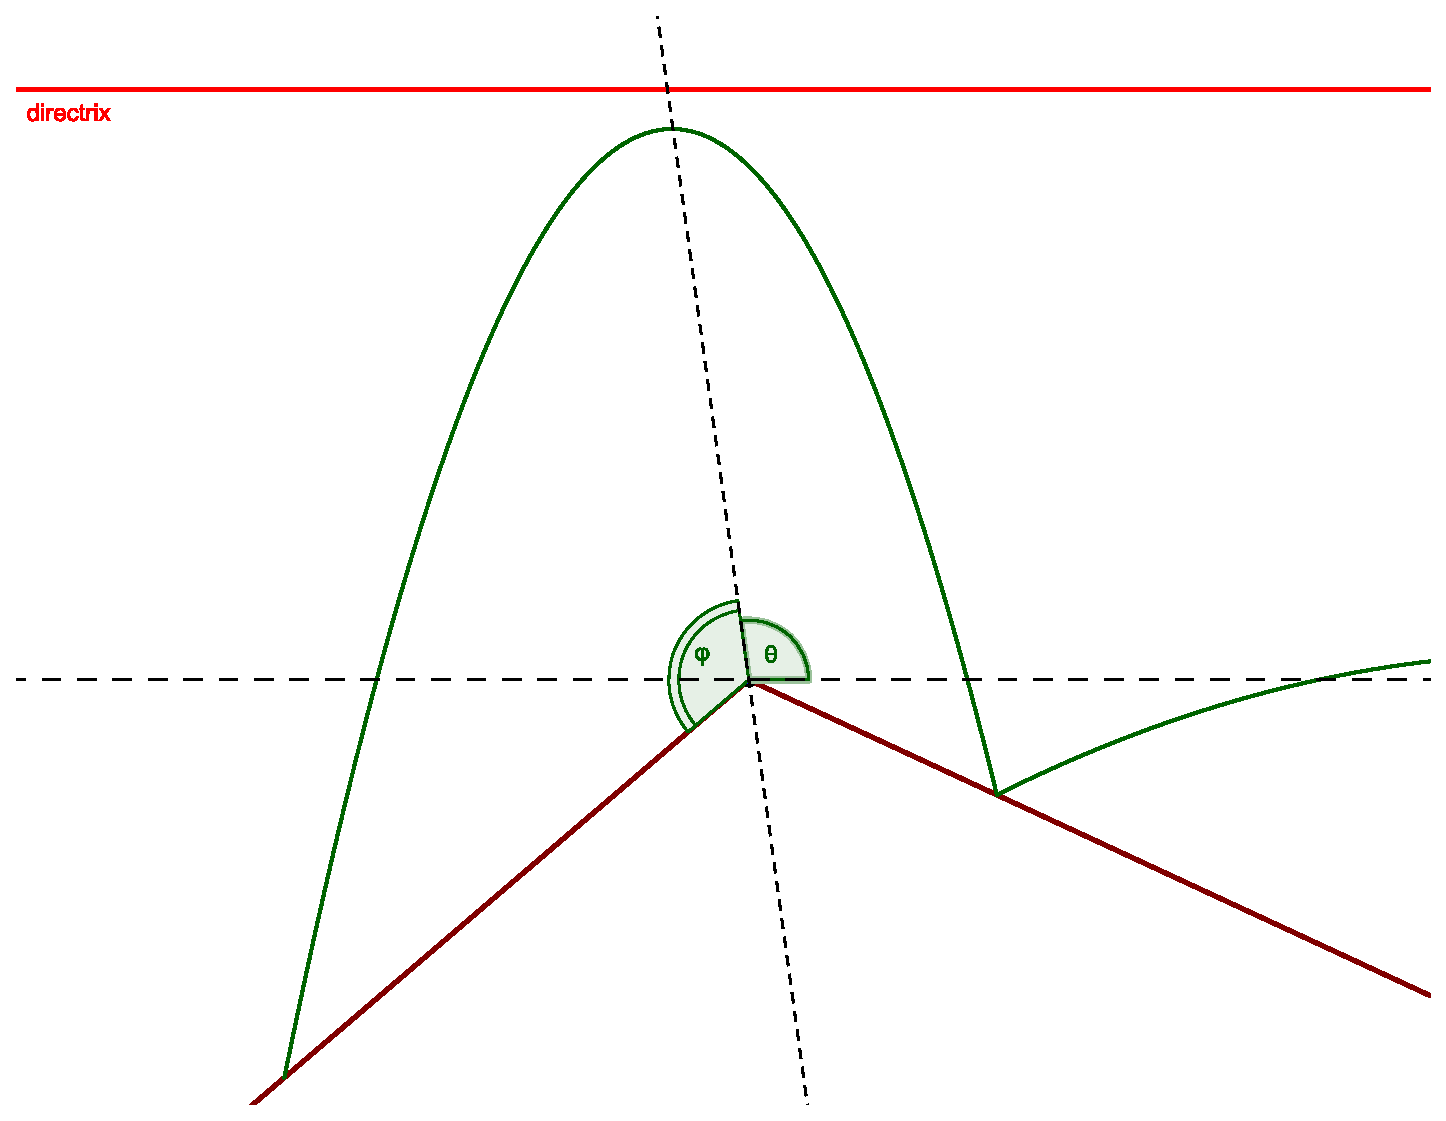
\includegraphics[width=95.7mm, height=125mm, viewport=3mm 4mm 205mm 292mm]{image13}\\
%   \caption{}\label{image13}
% \end{figure}

% Теперь удобно переписать  \eqref{GrindEQ__24_}, \ref{GrindEQ__25_} в терминах $\theta $ и $\varphi $, где ${{\alpha }_{1}}=\theta -\varphi $, ${{\alpha }_{2}}=\theta +\varphi $ и, соответственно, переименовывая индекс «1» и «2» как «$-$» и «$+$». Тогда
% \begin{equation} \label{GrindEQ__30_} \begin{array}{l}{d_ \pm } = \\4{\sin ^2}\left( {\theta  \pm \varphi } \right)\left( {1 - b \mp \left( {1 - b - {d_ \mp }\frac{{{{\left( {1 - {\tau _ \mp }} \right)}^2}}}{4}} \right)\frac{{\sin 4\varphi }}{{\sin 2\left( {\theta  \mp \varphi } \right)}} - \left( {1 - b - \frac{{{d_ \mp }}}{{4{{\sin }^2}\left( {\theta  \mp \varphi } \right)}}} \right)\frac{{\sin 2\left( {\theta  \pm \varphi } \right)}}{{\sin 2\left( {\theta  \mp \varphi } \right)}}} \right)\end{array} \end{equation}

% \begin{equation} \label{GrindEQ__31_}{\tau _ \pm } =  - 1 + \left( {1 - {\tau _ \mp }} \right)\frac{{\sin \left( {\theta  \pm \varphi } \right)}}{{\left| {\sin \left( {\theta  \pm \varphi } \right)} \right|}}\sqrt {\frac{{{d_ \mp }}}{{{d_ \pm }}}} \end{equation}
% Если теперь положить, что $-\pi \le \theta \le \pi$ и $0\le \varphi \le \pi$, то \eqref{GrindEQ__30_}, \eqref{GrindEQ__31_} также годится и для невыпуклых клиньев при ${\pi }/{2}\;\le \varphi \le \pi $ (см. Рис.\ref{image13})

\section{Выводы}

         В результате мы получили отображение, которое может использоваться не только для биллиарда в клине. Такой подход  можно расширить. Поскольку каждая плоская многоугольная фигура разбивается на участки в форме плоских клиньев, то для каждого из клиньев и пары его сторон мы можем задать углы, соответствующие движению внутри клина как описано выше. Для одной и той же стороны смежных клиньев мы должны задавать знаки отображения в соответствии с диаграммой на Рис. \ref{fig:angle_diagram2}. Таким образом, задавая знаки отображения для каждого клина, мы зададим параметры отображения для всей фигуры 
         
%(на Рис.\ref{image12} приведен пример для треугольника).

%\begin{figure}[ht]
%  \centering
%  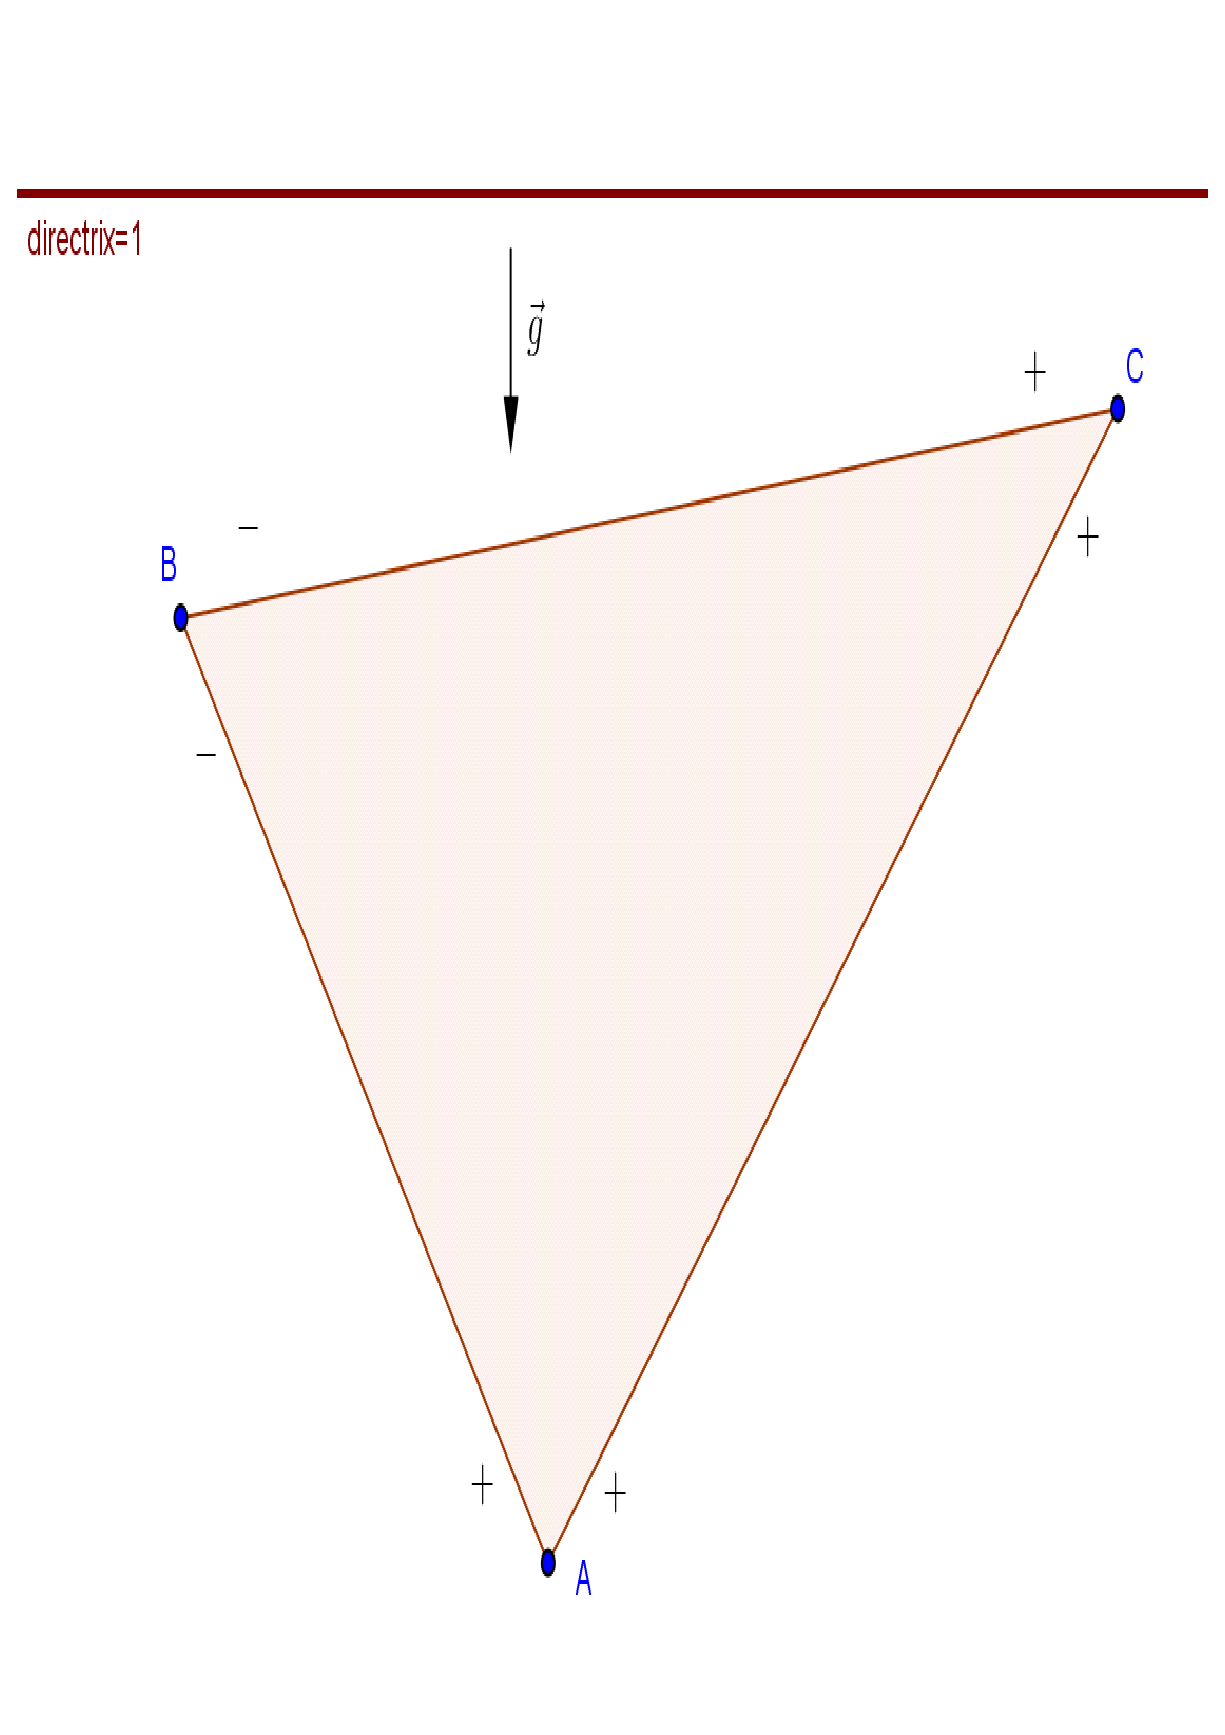
\includegraphics[width=95.7mm, height=69.9mm, viewport=3mm 4mm 205mm 292mm]{image12}\\
%  \caption{На рисунке через +/- отмечены знаки углов для отображения \eqref{GrindEQ__25_} в различных клиньях треугольника. В таком типе треугольника области определения для каждого из клиньев не пересекаются}\label{image12}
%\end{figure}

% На Рис.\ref{image12} через ${\raise0.7ex\hbox{$ + $}\!\mathord{\left/ {\vphantom {+ -}} \right. \kern-\nulldelimiterspace}\!\lower0.7ex\hbox{$ - $}}$ изображены знаки углов для отображения \eqref{GrindEQ__29_} в различных клиньях треугольника.
При этом возможна проблема пересечения клиньев. Т.е. могут появиться участки области определения фокусов, которые принадлежат более чем одному клину. Тогда выбор клина для следующего отображения будет уже не таким тривиальным. Но эту задачу еще предстоит решить. Однако уже сейчас можно констатировать, что описанный подход позволяет нам конструировать отображение для любых многоугольных плоских фигур, в том числе и невыпуклых.

Так же весьма интересна найденная связь между бильярдами типа $F$ и $C$. И хотя пока только для элементарного случая наклонной поверхности, вполне вероятно, что связь может быть на много глубже.

\begin{thebibliography}{31}
\bibitem{Lehtihet1986} Lehtihet, H.E. and Miller, B.N., Numerical study of a billiard in a gravitational field, Physica D: Nonlinear Phenomena, v.21, 1, p.93--104, 1986.

\bibitem{Sepulchre2003} R. Sepulchre and M. Gerard, Stabilization of periodic orbits in a wedge billiard, 42nd IEEE International Conference on Decision and Control (IEEE Cat. No.03CH37475), v.2, p.1568-1573, 2003.

\bibitem{Yanovskii2013} Yanovsky, V.V. and Tur, A.V. and Maslovsky, Yu.N., A charged composite particle in a constant electric field, Theoretical and Mathematical Physics, v.175, 2, p.655--680, 2013.

%\bibitem{}

%\bibitem{}

%\bibitem{}

%\bibitem{}

%\bibitem{}

%\bibitem{}

%\bibitem{}

%\bibitem{}

%\bibitem{}
\end{thebibliography}
\end{document}
